%%%%%%%%%%%%%%%%%%%%%%%%%%%%%%%%%%%%%%%%%%%%%%%%%%%%%%%%%%%%%%%%%%%%%%%%%%
%
% Copyright (c) 2008-2011, Nokia Corporation and/or its subsidiary(-ies).
% All rights reserved.
%
% This work, unless otherwise expressly stated, is licensed under a
% Creative Commons Attribution-ShareAlike 2.5.
%
% The full license document is available from
% http://creativecommons.org/licenses/by-sa/2.5/legalcode .
%
%%%%%%%%%%%%%%%%%%%%%%%%%%%%%%%%%%%%%%%%%%%%%%%%%%%%%%%%%%%%%%%%%%%%%%%%%%

% this is the driver for presentations
\documentclass[t]{beamer}
%%%%%%%%%%%%%%%%%%%%%%%%%%%%%%%%%%%%%%%%%%%%%%%%%%%%%%%%%%%%%%%%%%%%%%%%%%
%
% This work, unless otherwise expressly stated, is licensed under a
% Creative Commons Attribution-ShareAlike 2.5.
%
% The full license document is available from
% http://creativecommons.org/licenses/by-sa/2.5/legalcode .
%
%%%%%%%%%%%%%%%%%%%%%%%%%%%%%%%%%%%%%%%%%%%%%%%%%%%%%%%%%%%%%%%%%%%%%%%%%%

\usepackage{ifthen}

\newcommand{\coursetitle}{\title}
\newcommand{\producer}{\subtitle}
\newcommand{\material}{\institute}
\newcommand{\customer}{\author}
\newcommand{\partner}{\titlegraphic}

\newboolean{eval-version}
\newboolean{with-notes}
\newboolean{show-slide-id}
\newboolean{show-page-numbers}


%======================================================================
%                          Configuration of Title Page
%======================================================================


% General course title
\coursetitle{Qt Essentials}
\producer{\small{Training Course}}

% Presented for Customer or Presented by Trainer
\customer{Visit us at \url{http://qt-project.org}}

% Indicator for material version
\material{
  Produced by the Qt Training Partners \\
  \medskip
  \tiny{\textit{Material based on Qt 5.1, created on \today\\}}
}

% Partner company logo and name
% \partner{\includegraphics[height=2cm]{images/company} \\ The Partner}

%======================================================================
%                          Configuration of ifdefs
%======================================================================

%% Include ``Evaluation version'' on the slides?
\setboolean{eval-version}{false}

%% Whether to include instructors notes
\setboolean{with-notes}{false}

%% Should we show page numbers on in the footer?
\setboolean{show-page-numbers}{true}

%% Should we show slide-id's in the title?
\setboolean{show-slide-id}{false}

%% What is the screen resolution
\newcommand{\screenwidth}{1400}

%%%%%%%%%%%%%%%%%%%%%%%%%%%%%%%%%%%%%%%%%%%%%%%%%%%%%%%%%%%%%%%%%%%%%%%%%%
%
% Copyright (c) 2008-2011, Nokia Corporation and/or its subsidiary(-ies).
% All rights reserved.
%
% This work, unless otherwise expressly stated, is licensed under a
% Creative Commons Attribution-ShareAlike 2.5.
%
% The full license document is available from
% http://creativecommons.org/licenses/by-sa/2.5/legalcode .
%
%%%%%%%%%%%%%%%%%%%%%%%%%%%%%%%%%%%%%%%%%%%%%%%%%%%%%%%%%%%%%%%%%%%%%%%%%%

\usepackage{ifthen}
\usepackage{alltt}
\usepackage{comment}
\usepackage{multicol}
\usepackage{multirow}
\usepackage{hhline}
\usepackage{bold-extra}
\usepackage{version}
\usepackage{graphicx}
\usepackage{pgfpages}
\usepackage{picins}
\usepackage{makeidx}
\usepackage{multind}
\usepackage{xspace}
\usepackage{mathptmx}
\usepackage{pdfsync}
\usepackage{listings}
%\usepackage{multimedia}

\ifthenelse{\boolean{cc-license}}
{
  \usetheme{QtTraining}
} % else
{
  \usetheme{QtNokia}
}

% \definecolor{code_bg}{RGB}{255, 255, 204}

\lstdefinelanguage{qmake}%
  { morekeywords={SOURCES,HEADERS,RESOURCES,FORMS},
    morestring=[b]",
    sensitive=true,
    comment=[l]\#,
 }

\ifthenelse{\boolean{cc-license}}
{
  \lstdefinelanguage[Qt]{C++}[]{C++}%
{%
  morekeywords=[2]{%
    Q_OBJECT,Q_PROPERTY,%
    SIGNAL,SLOT,%
    signals,slots,connect,disconnect,%
    emit,tr,qobject_cast,foreach,%
    qscriptvalue_cast%
  },%
  %
  % Generated from Qt 4.7 include dir:
  % $ find . -name 'Q*' -printf '%f,%%\n'
  morekeywords=[3]{%
    QtUiTools,%
    QtUiTools,%
    QUiLoader,%
    QtNetwork,%
    QNetworkInterface,%
    QHostAddress,%
    QNetworkProxy,%
    QtNetwork,%
    QSsl,%
    QAuthenticator,%
    QSslCipher,%
    QNetworkAccessManager,%
    QAbstractSocket,%
    QNetworkRequest,%
    QLocalSocket,%
    QLocalServer,%
    QHttp,%
    QUdpSocket,%
    QTcpServer,%
    QTcpSocket,%
    QHttpResponseHeader,%
    QNetworkCookie,%
    QNetworkConfigurationManager,%
    QIPv6Address,%
    QSslCertificate,%
    QNetworkProxyFactory,%
    QUrlInfo,%
    QNetworkProxyQuery,%
    QNetworkAddressEntry,%
    QNetworkConfiguration,%
    QHostInfo,%
    QFtp,%
    QSslKey,%
    QSslError,%
    QNetworkCookieJar,%
    QNetworkReply,%
    QHttpHeader,%
    Q_IPV6ADDR,%
    QNetworkCacheMetaData,%
    QSslConfiguration,%
    QNetworkSession,%
    QNetworkDiskCache,%
    QSslSocket,%
    QHttpRequestHeader,%
    QAbstractNetworkCache,%
    Qt,%
    QtCore,%
    QMetaMethod,%
    QTextIStream,%
    QListIterator,%
    QBitArray,%
    QCoreApplication,%
    Q_INT32,%
    QForeachContainerBase,%
    QTextStream,%
    QFile,%
    QMetaObjectExtraData,%
    QFileInfoListIterator,%
    QThreadStorage,%
    QGlobalStatic,%
    QSysInfo,%
    QByteArray,%
    QStdWString,%
    QDebug,%
    QMutableFutureIterator,%
    QSettings,%
    Qt,%
    QAtomicPointer,%
    QProcess,%
    QLatin1Literal,%
    QThreadPool,%
    QChildEvent,%
    QReadLocker,%
    Q_LLONG,%
    QObjectCleanupHandler,%
    QtCore,%
    QHashIterator,%
    QStringRef,%
    QLocale,%
    Q_LONG,%
    QList,%
    QDir,%
    QResource,%
    QAnimationGroup,%
    QHashData,%
    QInternal,%
    QXmlStreamReader,%
    QMutableSetIterator,%
    QFuture,%
    QSetIterator,%
    QAbstractFileEngine,%
    QAbstractTableModel,%
    QRunnable,%
    QMapNode,%
    QtCleanUpFunction,%
    QStringList,%
    QEventTransition,%
    QTextStreamManipulator,%
    QPointer,%
    QContiguousCacheData,%
    Q_INT8,%
    QVector,%
    QXmlStreamEntityDeclarations,%
    QSharedDataPointer,%
    QtPlugin,%
    QTextBoundaryFinder,%
    QDateTime,%
    QMutableMapIterator,%
    QWeakPointer,%
    QPauseAnimation,%
    QVariantMap,%
    QExplicitlySharedDataPointer,%
    QXmlStreamWriter,%
    QStateMachine,%
    QDynamicPropertyChangeEvent,%
    QXmlStreamAttributes,%
    QPluginLoader,%
    QSize,%
    QPointF,%
    QBool,%
    QMetaObjectAccessor,%
    QLinkedListData,%
    Q_INT16,%
    QFinalState,%
    QSet,%
    QTextOStream,%
    QtConcurrentFilter,%
    QTextCodec,%
    QAbstractFileEngineIterator,%
    QSharedMemory,%
    QXmlStreamNamespaceDeclaration,%
    QVariantHash,%
    QHashDummyValue,%
    QReadWriteLock,%
    QObject,%
    QLinkedListIterator,%
    QSocketNotifier,%
    QConcatenable,%
    QMutableLinkedListIterator,%
    QVariant,%
    QTypeInfo,%
    QMargins,%
    QSystemSemaphore,%
    QIncompatibleFlag,%
    QMutableVectorIterator,%
    QtDebug,%
    QSequentialAnimationGroup,%
    QPersistentModelIndex,%
    Q_UINT32,%
    Q_ULLONG,%
    QScopedPointerDeleter,%
    QFutureInterface,%
    QMutableListIterator,%
    QMimeData,%
    QWaitCondition,%
    QBasicAtomicPointer,%
    QFileInfo,%
    QFileInfoList,%
    QTimeLine,%
    QMetaProperty,%
    QGenericArgument,%
    QTextDecoder,%
    QFactoryInterface,%
    QXmlStreamEntityResolver,%
    QVariantList,%
    QString,%
    QEasingCurve,%
    QMap,%
    QNoImplicitBoolCast,%
    QTemporaryFile,%
    QLinkedList,%
    QStringBuilder,%
    QTextEncoder,%
    QMetaObject,%
    QThreadStorageData,%
    QIODevice,%
    QAbstractFileEngineHandler,%
    QtEndian,%
    QVariantAnimation,%
    QScopedPointer,%
    QMetaClassInfo,%
    QFileSystemWatcher,%
    QLineF,%
    QtConfig,%
    QContiguousCacheTypedData,%
    QProcessEnvironment,%
    QForeachContainer,%
    QTS,%
    QVectorIterator,%
    QRectF,%
    QAtomicInt,%
    QtGlobal,%
    QVarLengthArray,%
    QByteRef,%
    QtConcurrentRun,%
    QCOORD,%
    QLatin1Char,%
    QStringListIterator,%
    QReturnArgument,%
    QDataStream,%
    QEventLoop,%
    QModelIndex,%
    QConstString,%
    QMetaTypeId,%
    QLibrary,%
    QParallelAnimationGroup,%
    QSharedPointer,%
    QVariantComparisonHelper,%
    QObjectUserData,%
    QTimer,%
    QCryptographicHash,%
    QThread,%
    QStringMatcher,%
    QXmlStreamAttribute,%
    QWriteLocker,%
    QHistoryState,%
    QQueue,%
    QtMsgHandler,%
    QElapsedTimer,%
    QSignalMapper,%
    QFSFileEngine,%
    QHashNode,%
    QUrl,%
    QFutureWatcherBase,%
    Q_ULONG,%
    QSizeF,%
    QAbstractConcatenable,%
    QByteArrayMatcher,%
    QFutureInterfaceBase,%
    QAbstractItemModel,%
    QTranslator,%
    QtPluginInstanceFunction,%
    QGlobalStaticDeleter,%
    QtConcurrentMap,%
    QNoDebug,%
    Q_UINT64,%
    QAbstractAnimation,%
    QObjectList,%
    QScopedPointerPodDeleter,%
    QMutexLocker,%
    QGenericReturnArgument,%
    QRect,%
    QPropertyAnimation,%
    QRegExp,%
    QMapData,%
    QXmlStreamNotationDeclaration,%
    QMultiMap,%
    QFutureSynchronizer,%
    QDirIterator,%
    QTextCodecPlugin,%
    QXmlStreamStringRef,%
    QMetaTypeId2,%
    QPair,%
    QHashDummyNode,%
    QLatin1String,%
    QModelIndexList,%
    QObjectData,%
    QXmlStreamNotationDeclarations,%
    QBasicAtomicInt,%
    QMutableHashIterator,%
    QMapPayloadNode,%
    QPoint,%
    QDate,%
    QSemaphore,%
    QIntegerForSize,%
    QLibraryInfo,%
    QBitRef,%
    QHash,%
    QMutex,%
    QArgument,%
    QMetaType,%
    QCache,%
    QtContainerFwd,%
    QTextCodecFactoryInterface,%
    QMutableStringListIterator,%
    QFutureWatcher,%
    QLinkedListNode,%
    Q_INT64,%
    QChar,%
    QFlags,%
    QUuid,%
    QLine,%
    QBasicTimer,%
    QStack,%
    QEvent,%
    QFutureIterator,%
    QScopedPointerArrayDeleter,%
    QVectorData,%
    QFlag,%
    Q_UINT16,%
    QSignalTransition,%
    QAbstractEventDispatcher,%
    QMapIterator,%
    QListData,%
    QMultiHash,%
    QTimerEvent,%
    QAbstractListModel,%
    Q_UINT8,%
    QState,%
    QScopedArrayPointer,%
    Q_PID,%
    QAbstractState,%
    QXmlStreamNamespaceDeclarations,%
    QTime,%
    QtAlgorithms,%
    QBuffer,%
    QCharRef,%
    QSharedData,%
    QVectorTypedData,%
    QSystemLocale,%
    QTextStreamFunction,%
    QAbstractTransition,%
    QCustomEvent,%
    QMetaEnum,%
    QContiguousCache,%
    QXmlStreamEntityDeclaration,%
    QtDesigner,%
    QDesignerWidgetDataBaseItemInterface,%
    QDesignerDynamicPropertySheetExtension,%
    QDesignerLanguageExtension,%
    QDesignerMetaDataBaseItemInterface,%
    QDesignerCustomWidgetCollectionInterface,%
    QtDesigner,%
    QDesignerIntegrationInterface,%
    QDesignerBrushManagerInterface,%
    QDesignerWidgetFactoryInterface,%
    QDesignerMemberSheetExtension,%
    QDesignerWidgetDataBaseInterface,%
    QDesignerDnDItemInterface,%
    QDesignerResourceBrowserInterface,%
    QDesignerPropertyEditorInterface,%
    QAbstractFormBuilder,%
    QDesignerFormWindowToolInterface,%
    QDesignerExtraInfoExtension,%
    QExtensionFactory,%
    QDesignerWidgetBoxInterface,%
    QDesignerActionEditorInterface,%
    QAbstractExtensionFactory,%
    QDesignerFormWindowManagerInterface,%
    QExtensionManager,%
    QDesignerFormWindowInterface,%
    QDesignerFormEditorInterface,%
    QDesignerFormEditorPluginInterface,%
    QFormBuilder,%
    QDesignerMetaDataBaseInterface,%
    QDesignerPromotionInterface,%
    QDesignerObjectInspectorInterface,%
    QDesignerExportWidget,%
    QDesignerLayoutDecorationExtension,%
    QDesignerPropertySheetExtension,%
    QDesignerFormWindowCursorInterface,%
    QAbstractExtensionManager,%
    QDesignerContainerExtension,%
    QDesignerTaskMenuExtension,%
    QDesignerComponents,%
    QDesignerCustomWidgetInterface,%
    QDesignerIconCacheInterface,%
    QtMultimedia,%
    QAudio,%
    QAbstractVideoSurface,%
    QAudioInput,%
    QAbstractVideoBuffer,%
    QtMultimedia,%
    QAbstractAudioInput,%
    QAudioEngineFactoryInterface,%
    QVideoSurfaceFormat,%
    QAbstractAudioDeviceInfo,%
    QAudioDeviceInfo,%
    QAudioFormat,%
    QAudioOutput,%
    QVideoFrame,%
    QAbstractAudioOutput,%
    QAudioEnginePlugin,%
    QAxFactory,%
    QAxSelect,%
    QAxObject,%
    QAxScriptManager,%
    QAxAggregated,%
    QAxBindable,%
    QAxScript,%
    QAxBase,%
    QAxScriptEngine,%
    QAxClass,%
    QAxWidget,%
    QtScript,%
    QScriptExtensionInterface,%
    QScriptContextInfo,%
    QScriptValueList,%
    QScriptProgram,%
    QtScript,%
    QScriptEngineAgent,%
    QScriptValue,%
    QScriptEngine,%
    QScriptable,%
    QScriptClassPropertyIterator,%
    QScriptContext,%
    QScriptExtensionPlugin,%
    QScriptSyntaxCheckResult,%
    QScriptValueIterator,%
    QScriptString,%
    QScriptContextInfoList,%
    QScriptClass,%
    QtMeeGoGraphicsSystemHelper,%
    QMeeGoLivePixmap,%
    QMeeGoOverlayWidget,%
    QMeeGoRuntime,%
    QtMeeGoGraphicsSystemHelper,%
    QMeeGoGraphicsSystemHelper,%
    QMeeGoLiveImage,%
    QtScriptTools,%
    QtScriptTools,%
    QScriptEngineDebugger,%
    QtSvg,%
    QSvgGenerator,%
    QSvgWidget,%
    QGraphicsSvgItem,%
    QtSvg,%
    QSvgRenderer,%
    QtSql,%
    QPSQLDriver,%
    QODBCResult,%
    QSqlDriver,%
    QSqlQuery,%
    QSqlResult,%
    QSqlTableModel,%
    QSqlRelationalTableModel,%
    QSQLiteDriver,%
    QIBaseDriver,%
    QSqlDriverCreatorBase,%
    QSQLiteResult,%
    QDB2Driver,%
    QMYSQLResult,%
    QtSql,%
    QSqlDatabase,%
    QTDSResult,%
    QSqlRelation,%
    QDB2Result,%
    QSqlIndex,%
    QIBaseResult,%
    QSqlField,%
    QSqlRecord,%
    QODBCDriver,%
    QSqlDriverFactoryInterface,%
    QPSQLResult,%
    QMYSQLDriver,%
    QSQLite2Result,%
    QSqlRelationalDelegate,%
    QOCIDriver,%
    QSQLite2Driver,%
    QOCIResult,%
    QSqlQueryModel,%
    QSqlDriverPlugin,%
    QTDSDriver,%
    QSqlDriverCreator,%
    QSqlError,%
    QtDBus,%
    QDBusReply,%
    QDBusServiceWatcher,%
    QDBusConnection,%
    QDBusError,%
    QDBusSignature,%
    QDBusMessage,%
    QDBusAbstractInterfaceBase,%
    QDBusContext,%
    QDBusServer,%
    QDBusConnectionInterface,%
    QDBusInterface,%
    QDBusPendingCallWatcher,%
    QDBusAbstractAdaptor,%
    QDBusPendingReplyData,%
    QDBusArgument,%
    QtDBus,%
    QDBusMetaType,%
    QDBusPendingCall,%
    QDBusVariant,%
    QDBusObjectPath,%
    QDBusAbstractInterface,%
    QDBusPendingReply,%
    QtGui,%
    QDragResponseEvent,%
    QWheelEvent,%
    QPrintDialog,%
    QTreeWidget,%
    QItemSelectionRange,%
    QGraphicsGridLayout,%
    QStandardItem,%
    QCalendarWidget,%
    QStyleOptionFocusRect,%
    QFormLayout,%
    QLinearGradient,%
    QItemSelectionModel,%
    QGraphicsColorizeEffect,%
    QWSServer,%
    QDialog,%
    QKeySequence,%
    QTextTable,%
    QWSKeyboardHandler,%
    QSyntaxHighlighter,%
    QRubberBand,%
    QAction,%
    QWSSoundServerSocket,%
    QWSInputMethod,%
    QItemEditorCreator,%
    QApplication,%
    QAuthDevice,%
    QTextBlockFormat,%
    QGraphicsEllipseItem,%
    QStyleOptionTabWidgetFrameV2,%
    QWSCursor,%
    QScrollBar,%
    QWSEvent,%
    QMouseDriverFactory,%
    QKbdDriverPlugin,%
    QUndoView,%
    QGradient,%
    QGraphicsRectItem,%
    QS60StubMAknTouchPaneObserver,%
    QGraphicsSceneContextMenuEvent,%
    QGroupBox,%
    QStyleOptionTabBarBaseV2,%
    QCDEStyle,%
    QPicture,%
    QScreenDriverFactory,%
    QColormap,%
    QStylePainter,%
    QIconDragEvent,%
    QWSQnxKeyboardHandler,%
    QWSScreenSaver,%
    QTableView,%
    QPrinterInfo,%
    QGraphicsPolygonItem,%
    QMotifStyle,%
    QTabBar,%
    QAccessibleInterfaceEx,%
    QFrame,%
    QTextLine,%
    QAccessibleSimpleEditableTextInterface,%
    QPolygonF,%
    QGraphicsOpacityEffect,%
    QMovie,%
    QDesktopServices,%
    QGraphicsLineItem,%
    QAccessibleFactoryInterface,%
    QPaintEngine,%
    QPixmapCache,%
    QCommonStyle,%
    QMatrix3x4,%
    QWhatsThisClickedEvent,%
    QInputEvent,%
    QGraphicsRotation,%
    QGraphicsSceneHelpEvent,%
    QSystemTrayIcon,%
    QStyleOptionViewItemV3,%
    QGraphicsTransform,%
    QLinuxFb_Shared,%
    QMatrix2x4,%
    QGraphicsAnchor,%
    QProgressBar,%
    QPrintEngine,%
    QSizePolicy,%
    QMenubarUpdatedEvent,%
    QMenuItem,%
    QContextMenuEvent,%
    QAccessibleActionInterface,%
    QPushButton,%
    QStyledItemDelegate,%
    QWSCursorMap,%
    QTapAndHoldGesture,%
    QDirectPainter,%
    QWidgetSet,%
    QItemSelection,%
    QS60MainApplicationBase,%
    QTableWidget,%
    QAbstractScrollArea,%
    QPaintEvent,%
    QAccessibleBridge,%
    QTextTableCell,%
    QToolTip,%
    QMimeSource,%
    QDecorationDefault,%
    QDoubleSpinBox,%
    QVector3D,%
    QGraphicsView,%
    QDragMoveEvent,%
    QVFbMouseHandler,%
    QStyleOptionDockWidget,%
    QGraphicsDropShadowEffect,%
    QTextBrowser,%
    QColorDialog,%
    QCompleter,%
    QDecoration,%
    QWindowsStyle,%
    QMenuBar,%
    QAccessibleWidgetEx,%
    QPinchGesture,%
    QLayoutIterator,%
    QWidget,%
    QImageReader,%
    QToolBar,%
    QMacMime,%
    QPlainTextDocumentLayout,%
    QImageWriter,%
    QDial,%
    QGtkStyle,%
    QStyleOptionMenuItem,%
    QWindowsMobileStyle,%
    QStyleOptionQ3DockWindow,%
    QInputContext,%
    QVFbKeyboardHandler,%
    QTextBlockGroup,%
    QColor,%
    QStyleFactoryInterface,%
    QTreeView,%
    QGraphicsPathItem,%
    QTreeWidgetItem,%
    QPrintPreviewWidget,%
    QInputContextPlugin,%
    QToolBarChangeEvent,%
    QPixmap,%
    QStyleOptionButton,%
    QBoxLayout,%
    QWSServerSocket,%
    QActionGroup,%
    QWSPropertyManager,%
    QStyleOptionProgressBarV2,%
    QDateTimeEdit,%
    QX11EmbedContainer,%
    QTextCharFormat,%
    QClipboardEvent,%
    QKbdDriverFactory,%
    QScrollArea,%
    QDragEnterEvent,%
    QStyleOptionQ3ListView,%
    QTextBlockUserData,%
    QTextImageFormat,%
    QStyleOptionComboBox,%
    QVector4D,%
    QLayoutItem,%
    QStyleOptionTabBarBase,%
    QMacNativeWidget,%
    QValidator,%
    QInputDialog,%
    QStyleOptionGraphicsItem,%
    QStandardItemModel,%
    QTextEdit,%
    QWSClient,%
    QStyleOptionSlider,%
    QPrinter,%
    QTextDocumentFragment,%
    QStyleOptionToolButton,%
    QWSSoundClient,%
    QTableWidgetItem,%
    QMatrix3x3,%
    QGraphicsObject,%
    QCommandLinkButton,%
    QS60MainApplication,%
    QStyleOptionComplex,%
    QWindowStateChangeEvent,%
    QAbstractSpinBox,%
    QFileSystemModel,%
    QGraphicsSceneMoveEvent,%
    QTreeWidgetItemIterator,%
    QScreen,%
    QDoubleValidator,%
    QTextListFormat,%
    QScreenDriverFactoryInterface,%
    QS60StubAknAppUi,%
    QMatrix2x3,%
    QDropEvent,%
    QGraphicsLayout,%
    QGestureRecognizer,%
    QGraphicsLinearLayout,%
    QStyleOptionToolBoxV2,%
    QAccessibleWidget,%
    QTransportAuth,%
    QWidgetItem,%
    QDragLeaveEvent,%
    QClipboard,%
    QHeaderView,%
    QTextDocumentWriter,%
    QPalette,%
    QItemEditorFactory,%
    QDecorationFactory,%
    QMainWindow,%
    QGraphicsSceneMouseEvent,%
    QColumnView,%
    QMatrix,%
    QGraphicsSceneEvent,%
    QMdiArea,%
    QTextObjectInterface,%
    QTextLayout,%
    QIcon,%
    QStyleOptionFrameV3,%
    QFocusEvent,%
    QAbstractGraphicsShapeItem,%
    QPainterPathStroker,%
    QShortcutEvent,%
    QSplitterHandle,%
    QTextTableCellFormat,%
    QTextBlock,%
    QRadioButton,%
    QAccessibleObject,%
    QIconEngineFactoryInterface,%
    QStyleOptionViewItemV2,%
    QGesture,%
    QStyleOptionToolBar,%
    QLCDNumber,%
    QProxyModel,%
    QSplitter,%
    QLineEdit,%
    QDialogButtonBox,%
    QFocusFrame,%
    QStyle,%
    QS60Style,%
    QFontInfo,%
    QWSProtocolItem,%
    QCursor,%
    QScreenDriverPlugin,%
    QAccessibleImageInterface,%
    QGradientStop,%
    QS60MainAppUiBase,%
    QDateEdit,%
    QTabletEvent,%
    QScreenCursor,%
    QTextFrame,%
    QWindowsCEStyle,%
    QWSMouseHandlerFactoryInterface,%
    QLabel,%
    QDecorationWindows,%
    QAbstractItemView,%
    QStyleOptionHeader,%
    QProgressDialog,%
    QPolygon,%
    QAccessibleTableInterface,%
    QStyleOptionTitleBar,%
    QFontMetricsF,%
    QMenu,%
    QGraphicsItemAnimation,%
    QWidgetList,%
    QAbstractPageSetupDialog,%
    QIntValidator,%
    QGraphicsSceneWheelEvent,%
    QTextInlineObject,%
    QStyleOptionTabWidgetFrame,%
    QWorkspace,%
    QPictureFormatInterface,%
    QWSUmKeyboardHandler,%
    QItemDelegate,%
    QAccessibleTextInterface,%
    QPaintEngineState,%
    QGenericMatrix,%
    QHBoxLayout,%
    QBrushData,%
    QRegExpValidator,%
    QX11EmbedWidget,%
    QAbstractFontEngine,%
    QAccessibleObjectEx,%
    QTextFormat,%
    QMatrix4x2,%
    QTextFragment,%
    QBrush,%
    QTransform,%
    QS60MainAppUi,%
    QAbstractSlider,%
    QStyleOptionTabV3,%
    QListWidgetItem,%
    QTapGesture,%
    QUndoGroup,%
    QTextOption,%
    QResizeEvent,%
    QStyleOptionViewItemV4,%
    QImage,%
    QWSMouseHandler,%
    QWSLinuxInputKeyboardHandler,%
    QX11Info,%
    QGraphicsAnchorLayout,%
    QFileOpenEvent,%
    QImageIOHandlerFactoryInterface,%
    QTextCursor,%
    QDecorationPlugin,%
    QVector2D,%
    QDrag,%
    QPainterPath,%
    QItemEditorCreatorBase,%
    QAccessibleEvent,%
    QStatusTipEvent,%
    QStylePlugin,%
    QStyleFactory,%
    QPainter,%
    QAccessibleApplication,%
    QListWidget,%
    QWMatrix,%
    QAccessible2Interface,%
    QTextTableFormat,%
    QTextLength,%
    QAccessibleInterface,%
    QProxyScreen,%
    QUnixPrintWidget,%
    QUndoStack,%
    QTransformedScreen,%
    QS60MainDocumentBase,%
    QSplashScreen,%
    QUpdateLaterEvent,%
    QDecorationFactoryInterface,%
    QAccessibleBridgeFactoryInterface,%
    QStyleHintReturnVariant,%
    QImageIOHandler,%
    QStyleOptionViewItem,%
    QWidgetAction,%
    QStandardItemEditorCreator,%
    QGraphicsLayoutItem,%
    QKeyEventTransition,%
    QAbstractPrintDialog,%
    QStyleOptionDockWidgetV2,%
    QAbstractProxyModel,%
    QS60StubMEikStatusPaneObserver,%
    QSwipeGesture,%
    QGestureEvent,%
    QShortcut,%
    QMacPasteboardMime,%
    QTabWidget,%
    QMouseDriverPlugin,%
    QMacStyle,%
    QAbstractTextDocumentLayout,%
    QWSInternalWindowInfo,%
    QWSDisplay,%
    QTextObject,%
    QTextFrameFormat,%
    QTableWidgetSelectionRange,%
    QFontEngineInfo,%
    QMatrix3x2,%
    QAccessibleValueInterface,%
    QPaintDevice,%
    QMouseEventTransition,%
    QWSKeyboardHandlerFactoryInterface,%
    QSound,%
    QGraphicsItemGroup,%
    QGraphicsSceneHoverEvent,%
    QAbstractUndoItem,%
    QSizeGrip,%
    QRgb,%
    QWidgetData,%
    QVFbHeader,%
    QStyleOptionRubberBand,%
    QAccessiblePlugin,%
    QGraphicsWidget,%
    QIconSet,%
    QStyleOptionFrameV2,%
    QPlainTextEdit,%
    QToolBox,%
    QHideEvent,%
    QCopChannel,%
    QStackedLayout,%
    QProxyScreenCursor,%
    QCleanlooksStyle,%
    QWSManager,%
    QMessageBox,%
    QWSSocket,%
    QTextItem,%
    QStyleOptionToolBox,%
    QWidgetItemV2,%
    QS60StubAknAppUiBase,%
    QStaticText,%
    QQnxMouseHandler,%
    QStyleOptionProgressBar,%
    QPictureIO,%
    QConicalGradient,%
    QPen,%
    QS60MainDocument,%
    QMacCocoaViewContainer,%
    QGridLayout,%
    QIconEnginePlugin,%
    QtGui,%
    QWSPointerCalibrationData,%
    QFont,%
    QSessionManager,%
    QRegion,%
    QGraphicsSimpleTextItem,%
    QStyleOption,%
    QWSWindow,%
    QImageIOPlugin,%
    QMatrix4x4,%
    QGradientStops,%
    QLayout,%
    QWhatsThis,%
    QMoveEvent,%
    QIconEngineFactoryInterfaceV2,%
    QTextDocument,%
    QCloseEvent,%
    QInputContextFactory,%
    QWizard,%
    QWSCalibratedMouseHandler,%
    QQuaternion,%
    QInputContextFactoryInterface,%
    QGraphicsEffect,%
    QPoolEntry,%
    QFileIconProvider,%
    QIconEngineV2,%
    QShowEvent,%
    QAbstractItemDelegate,%
    QQnxScreen,%
    QHelpEvent,%
    QDockWidget,%
    QStyleOptionFrame,%
    QSlider,%
    QWSWindowInfo,%
    QHoverEvent,%
    QWizardPage,%
    QVFbScreen,%
    QDecorationStyled,%
    QSpacerItem,%
    QMdiSubWindow,%
    QFontComboBox,%
    QGraphicsBlurEffect,%
    QWSTslibMouseHandler,%
    QStyleOptionQ3ListViewItem,%
    QTimeEdit,%
    QGraphicsProxyWidget,%
    QTileRules,%
    QMatrix2x2,%
    QVFbKeyData,%
    QFontEngineFactoryInterface,%
    QIconEnginePluginV2,%
    QAccessibleBridgePlugin,%
    QStringListModel,%
    QStyleOptionSpinBox,%
    QStyleHintReturnMask,%
    QCheckBox,%
    QtEvents,%
    QWSTtyKeyboardHandler,%
    QGraphicsItem,%
    QPageSetupDialog,%
    QWSLinuxInputMouseHandler,%
    QMatrix4x3,%
    QWSSoundServer,%
    QGraphicsTextItem,%
    QGraphicsSceneResizeEvent,%
    QGraphicsScene,%
    QTextFrameLayoutData,%
    QDesktopWidget,%
    QTouchEvent,%
    QColorGroup,%
    QRadialGradient,%
    QWindowsMime,%
    QToolButton,%
    QPlastiqueStyle,%
    QButtonGroup,%
    QDecorationAction,%
    QPainterPathPrivate,%
    QDirModel,%
    QSortFilterProxyModel,%
    QWindowsVistaStyle,%
    QActionEvent,%
    QStyleOptionTabV2,%
    QStackedWidget,%
    QStatusBar,%
    QStyleOptionGroupBox,%
    QGraphicsSceneDragDropEvent,%
    QComboBox,%
    QStyleOptionSizeGrip,%
    QIconEngine,%
    QLinuxFbScreen,%
    QProxyStyle,%
    QKeyEvent,%
    QPictureFormatPlugin,%
    QFontDatabase,%
    QErrorMessage,%
    QInputMethodEvent,%
    QPanGesture,%
    QDataWidgetMapper,%
    QWidgetMapper,%
    QWSPcMouseHandler,%
    QBitmap,%
    QCursorShape,%
    QPrintPreviewDialog,%
    QAccessibleEditableTextInterface,%
    QAccessible,%
    QFontDialog,%
    QTextList,%
    QMouseEvent,%
    QStyleOptionTab,%
    QSpinBox,%
    QWSEmbedWidget,%
    QStyleHintReturn,%
    QGraphicsPixmapItem,%
    QAbstractButton,%
    QWindowsXPStyle,%
    QWSLinuxTPMouseHandler,%
    QImageTextKeyLang,%
    QListView,%
    QFontMetrics,%
    QSymbianEvent,%
    QUndoCommand,%
    QFontEnginePlugin,%
    QGraphicsScale,%
    QFileDialog,%
    QVBoxLayout,%
    QtDeclarative,%
    QDeclarativeExpression,%
    QDeclarativeListReference,%
    QDeclarativeAttachedPropertiesFunc,%
    QDeclarativeEngine,%
    QDeclarativeListProperty,%
    QDeclarativeError,%
    QDeclarativeComponent,%
    QDeclarativeScriptString,%
    QDeclarativeExtensionInterface,%
    QDeclarativeImageProvider,%
    QDeclarativePropertyValueInterceptor,%
    QDeclarativeProperties,%
    QDeclarativeContext,%
    QDeclarativeItem,%
    QDeclarativePropertyValueSource,%
    QDeclarativeView,%
    QDeclarativeTypeInfo,%
    QtDeclarative,%
    QDeclarativeExtensionPlugin,%
    QDeclarativeProperty,%
    QDeclarativeInfo,%
    QDeclarativePropertyMap,%
    QDeclarativeParserStatus,%
    QDeclarativeNetworkAccessManagerFactory,%
    QtTest,%
    QTestMouseEvent,%
    QTestLightXmlStreamer,%
    QTestFileLogger,%
    QTestData,%
    QTestXunitStreamer,%
    QSpontaneKeyEvent,%
    QTestEvent,%
    QTestEventList,%
    QEventSizeOfChecker,%
    QTestAccessibility,%
    QTestKeyClicksEvent,%
    QTestElementAttribute,%
    QTestAccessibilityEvent,%
    QTestCoreList,%
    QTestXmlStreamer,%
    QTestElement,%
    QTestBasicStreamer,%
    QSignalSpy,%
    QTestEventLoop,%
    QtTest,%
    QtTestGui,%
    QTestCoreElement,%
    QTest,%
    QTestKeyEvent,%
    QTestDelayEvent,%
    QtXml,%
    QDomNotation,%
    QDomImplementation,%
    QXmlDefaultHandler,%
    QXmlStreamReader,%
    QXmlInputSource,%
    QXmlStreamEntityDeclarations,%
    QXmlStreamWriter,%
    QXmlStreamAttributes,%
    QXmlReader,%
    QXmlNamespaceSupport,%
    QXmlDTDHandler,%
    QXmlLocator,%
    QDomNode,%
    QDomProcessingInstruction,%
    QXmlStreamNamespaceDeclaration,%
    QDomElement,%
    QXmlErrorHandler,%
    QDomDocumentFragment,%
    QXmlStreamEntityResolver,%
    QDomNamedNodeMap,%
    QDomAttr,%
    QXmlDeclHandler,%
    QDomEntity,%
    QXmlLexicalHandler,%
    QDomNodeList,%
    QDomCharacterData,%
    QXmlEntityResolver,%
    QXmlSimpleReader,%
    QXmlStreamAttribute,%
    QDomDocumentType,%
    QDomEntityReference,%
    QDomCDATASection,%
    QXmlStreamNotationDeclaration,%
    QXmlAttributes,%
    QXmlStreamStringRef,%
    QXmlStreamNotationDeclarations,%
    QtXml,%
    QDomComment,%
    QDomDocument,%
    QXmlContentHandler,%
    QXmlStreamNamespaceDeclarations,%
    QDomText,%
    QXmlParseException,%
    QXmlStreamEntityDeclaration,%
    QtWebKit,%
    QWebElement,%
    QWebSecurityOrigin,%
    QWebElementCollection,%
    QWebHistoryItem,%
    QGraphicsWebView,%
    QWebHistory,%
    QWebPage,%
    QWebFrame,%
    QWebSettings,%
    QWebHitTestResult,%
    QWebInspector,%
    QWebPluginFactory,%
    QWebDatabase,%
    QtWebKit,%
    QWebHistoryInterface,%
    QWebView,%
    Qt3Support,%
    Q3Button,%
    Q3SocketDevice,%
    Q3ProgressDialog,%
    Q3DataTable,%
    Q3IconDrag,%
    Q3HttpResponseHeader,%
    Q3GridLayout,%
    Q3ListBox,%
    Q3SqlFieldInfoList,%
    Q3DataBrowser,%
    Q3PaintDeviceMetrics,%
    Q3CanvasPolygon,%
    Q3PtrQueue,%
    Q3NetworkProtocolFactoryBase,%
    Q3SortedList,%
    Q3SingleCleanupHandler,%
    Q3NetworkOperation,%
    Q3PtrDictIterator,%
    Q3ObjectDictionary,%
    Q3CString,%
    Q3TextStream,%
    Q3DateTimeEdit,%
    Q3ButtonGroup,%
    Q3VBox,%
    Q3AsciiBucket,%
    Q3CanvasSprite,%
    Q3CanvasRectangle,%
    Q3HttpRequestHeader,%
    Q3UriDrag,%
    Q3CanvasPixmap,%
    Q3HBox,%
    Q3AsciiCache,%
    Q3GCacheIterator,%
    Q3GVector,%
    Q3ToolBar,%
    Q3NetworkProtocolFactory,%
    Q3GCache,%
    Q3CanvasText,%
    Q3IntDictIterator,%
    Q3VButtonGroup,%
    Q3TabDialog,%
    Q3UrlOperator,%
    Q3Action,%
    Q3TextEditOptimPrivate,%
    Q3SyntaxHighlighter,%
    Q3TableSelection,%
    Q3Http,%
    Q3GListStdIterator,%
    Q3GList,%
    Q3StrIList,%
    Q3PtrDict,%
    Q3PtrCollection,%
    Q3StyleSheetItem,%
    Q3GridView,%
    Q3ListViewItemIterator,%
    Q3LNode,%
    Q3Url,%
    Q3CanvasLine,%
    Q3ValueListConstIterator,%
    Q3FileDialog,%
    Q3EditorFactory,%
    Q3ComboBox,%
    Q3VBoxLayout,%
    Q3ProgressBar,%
    Q3Signal,%
    Q3HGroupBox,%
    Q3Picture,%
    Q3DragObject,%
    Q3PtrBucket,%
    Q3CanvasSpline,%
    Q3Accel,%
    Q3VGroupBox,%
    Q3DataView,%
    Q3CleanupHandler,%
    Q3TableItem,%
    Q3SqlRecordInfo,%
    Q3StrList,%
    Q3Ftp,%
    Q3IntCache,%
    Q3CheckListItem,%
    Q3StyleSheet,%
    Q3HBoxLayout,%
    Q3IntDict,%
    Q3FilePreview,%
    Q3DateTimeEditBase,%
    Q3Frame,%
    Q3AsciiDictIterator,%
    Q3GDict,%
    Q3ListViewItem,%
    Q3StoredDrag,%
    Q3StrListIterator,%
    Q3CanvasView,%
    Q3PtrStack,%
    Q3CacheIterator,%
    Q3SqlForm,%
    Q3RangeControl,%
    Q3Dns,%
    Q3Dict,%
    Q3ColorDrag,%
    Q3TextView,%
    Q3ValueListIterator,%
    Q3IntCacheIterator,%
    Q3Table,%
    Q3ComboTableItem,%
    Q3ScrollView,%
    Q3ListBoxPixmap,%
    Q3PopupMenu,%
    Q3SqlSelectCursor,%
    Q3DictIterator,%
    Q3ValueList,%
    Q3CanvasPolygonalItem,%
    Q3DateEdit,%
    Q3StrVec,%
    Q3GroupBox,%
    Q3DropSite,%
    Q3DnsSocket,%
    Q3PtrListStdIterator,%
    Q3WhatsThis,%
    Q3GDictIterator,%
    Q3DeepCopy,%
    Q3Cache,%
    Q3SimpleRichText,%
    Q3ListBoxText,%
    Q3IconViewItem,%
    Q3Grid,%
    Q3SpinWidget,%
    Q3BaseBucket,%
    Q3Painter,%
    Q3Header,%
    Q3NetworkProtocolDict,%
    Q3DockArea,%
    Q3Wizard,%
    Q3PtrList,%
    Q3MultiLineEdit,%
    Q3Shared,%
    Q3PointArray,%
    Q3ListBoxItem,%
    Q3ListView,%
    Q3ValueVector,%
    Q3WidgetStack,%
    Q3ServerSocket,%
    Q3MemArray,%
    Q3TimeEdit,%
    Q3AsciiCacheIterator,%
    Q3TSFUNC,%
    Q3HButtonGroup,%
    Q3CanvasItemList,%
    Q3AsciiDict,%
    Q3DockAreaLayout,%
    Q3IconDragItem,%
    Q3SqlEditorFactory,%
    Q3SqlPropertyMap,%
    Q3PtrVector,%
    Q3GListIterator,%
    Q3StrIVec,%
    Q3IntBucket,%
    Q3BoxLayout,%
    Q3CanvasItem,%
    Q3TextDrag,%
    Q3MainWindow,%
    Q3TextBrowser,%
    Q3GArray,%
    Q3PtrListIterator,%
    Q3CheckTableItem,%
    Q3HttpHeader,%
    Q3SqlFieldInfo,%
    Q3Socket,%
    Q3MimeSourceFactory,%
    Qt3Support,%
    Q3FileIconProvider,%
    Q3SqlCursor,%
    Q3StringBucket,%
    Q3CanvasPixmapArray,%
    Q3LocalFs,%
    Q3TextEdit,%
    Q3PolygonScanner,%
    Q3ActionGroup,%
    Q3NetworkProtocol,%
    Q3ValueStack,%
    Q3ImageDrag,%
    Q3Semaphore,%
    Q3CanvasEllipse,%
    Q3Canvas,%
    Q3DockWindow,%
    Q3IconView,%
    Q3Process,%
    QtXmlPatterns,%
    QXmlSerializer,%
    QXmlQuery,%
    QXmlNodeModelIndex,%
    QXmlSchema,%
    QXmlNamePool,%
    QXmlResultItems,%
    QSimpleXmlNodeModel,%
    QAbstractXmlNodeModel,%
    QSourceLocation,%
    QAbstractUriResolver,%
    QXmlSchemaValidator,%
    QXmlFormatter,%
    QXmlItem,%
    QXmlName,%
    QAbstractMessageHandler,%
    QtXmlPatterns,%
    QAbstractXmlReceiver,%
    QtHelp,%
    QHelpContentItem,%
    QHelpContentWidget,%
    QHelpEngine,%
    QHelpEngineCore,%
    QHelpSearchQuery,%
    QHelpIndexModel,%
    QHelpSearchResultWidget,%
    QHelpIndexWidget,%
    QHelpContentModel,%
    QHelpSearchEngine,%
    QHelpGlobal,%
    QHelpSearchQueryWidget,%
    QtHelp,%
    QtOpenVG,%
    QtOpenVG,%
    QtOpenGL,%
    QMacCompatGLenum,%
    QGLBuffer,%
    QGLPixelBuffer,%
    QGLColormap,%
    QMacCompatGLuint,%
    QGLFramebufferObjectFormat,%
    QGLScreenSurfaceFunctions,%
    QGLContext,%
    QGLFramebufferObject,%
    QGLScreen,%
    QGLWidget,%
    QMacGLCompatTypes,%
    QMacCompatGLint,%
    QGLShader,%
    QGLFormat,%
    QGLShaderProgram,%
    QtOpenGL%
  }
}


  \definecolor{devnet_magenta} {RGB}{255, 20,147} % {216,  0,117}
  \definecolor{devnet_green}   {RGB}{108,226,108} % { 58,216, 58}
  \definecolor{devnet_gray}    {RGB}{175,175,175} % {145,145,145}
  \definecolor{devnet_silver}  {RGB}{128,128,128} % { 98, 98, 98}
  \definecolor{devnet_blue}    {RGB}{  0,102,153} % {  0, 61, 92}
  \definecolor{devnet_fullblue}{RGB}{  0,  0,255} % {  0,  0,225}
  \definecolor{devnet_qtgreen} {RGB}{  0,130,  0} % {  0,100,  0}
                                                  % -30 lum points
  \lstset{ %
    language=[Qt]C++,
    basicstyle=\ttfamily\footnotesize,
    keywordstyle=\bfseries\color{devnet_blue},
    keywordstyle=[2]\bfseries\color{devnet_blue},
    keywordstyle=[3]\bfseries\color{devnet_magenta},
    stringstyle=\color{devnet_fullblue},
    commentstyle=\color{devnet_qtgreen},
    %numbers=left,
    %numberstyle=\tiny,
    %stepnumber=1,
    %numbersep=10pt,
    showspaces=false,
    showstringspaces=false,
    frame=l,
    framerule=1pt,
    framesep=4pt,
    %rulecolor=\color{black!30},
    rulecolor=\color{devnet_qtgreen},
    aboveskip=1mm,
    belowskip=1mm,
    showlines=false,
  }
}
{
  \lstdefinelanguage[Qt]{C++}[]{C++}%
  { keywordsprefix=Q
  }

  \lstset{ % 
    language=[Qt]C++,
    basicstyle=\ttfamily\footnotesize,
    keywordstyle=\bfseries,
    stringstyle=\color{blue},
    commentstyle=\color{qtlightgreen}, 
    %numbers=left,
    %numberstyle=\tiny,
    %stepnumber=1,
    %numbersep=10pt, 
    showspaces=false,
    showstringspaces=false,
    frame=l, 
    framerule=1pt,
    framesep=4pt,
    %rulecolor=\color{black!30},
    rulecolor=\color{qtlightgreen},
    aboveskip=1mm,
    belowskip=1mm,
    showlines=false,
  }
}

\lstnewenvironment{cpp}{\lstset{language=[Qt]C++}}{}
\lstnewenvironment{qmake}{\lstset{language=qmake}}{}
\lstnewenvironment{shell}{\lstset{language=bash}}{}
\lstnewenvironment{xml}{\lstset{language=html}}{}


\newcommand{\inputqml}[1]{%
\setlength{\lineskip}{0pt}
\footnotesize
\input{#1}
\normalsize
}

\newenvironment{qml}{%
\setlength{\lineskip}{0pt}
\footnotesize
}{%
}

\newcommand{\qthome}[2]{\href{http://qt.nokia.com/#1}{\beamerbutton{See #2}}}  
\newcommand{\doc}[2]{\href{http://qt.nokia.com/doc/latest/#1}{\beamerbutton{See #2 Documentation}}}  
\newcommand{\wiki}[2]{\href{http://en.wikipedia.org/wiki/#1}{\beamerbutton{See #2 Wikipedia Article}}}  
\newcommand{\doccreator}[2]{\href{http://doc.qt.nokia.com/qtcreator/#1}{\beamerbutton{See #2 Documentation}}}  
\newcommand{\demo}[1]{\href{run:#1}{\beamerbutton{Demo #1}}}  
\newcommand{\qtdemo}[1]{\href{run:#1}{\beamerbutton{Demo \$QTDIR/#1}}}  
\newcommand{\lab}[1]{\href{run:#1}{\beamerbutton{Lab #1}}}
\newcommand\externalLink[1]{{\sffamily\color{blue}{\href{#1}{#1}}}}
\newcommand\externalNamedLink[2]{{\sffamily\color{blue}{\href{#1}{#2}}}}


\date{}

\sloppy
\newenvironment{answers}[2]{%
\begin{frame}[fragile]
\begin{center}
#1\\(page #2)
\end{center}
\tiny
}{%
\end{frame}}

%----------------------------------------------------------------------

% setup for two column printing.
\setlength{\columnseprule}{1pt}
\setlength{\columnsep}{20pt}

%----------------------------------------------------------------------
\newcommand{\secTitle}{}
\newcommand{\setSectionTitle}[1]{\def\secTitle{#1}\section{#1}}
\newcommand{\sectionTitle}{\secTitle}

\newcommand{\contentHyperlink}[2]{\hyperlink{#2}{#1 (page~\pageref{#2})}}
\newcommand{\pageHyperlink}[1]{\hyperlink{#1}{page~\pageref{#1}}}
\newcommand{\itop}[2]{\item \contentHyperlink{#1}{#2}}
\newcommand{\itopStar}[2]{\item<*> \contentHyperlink{#1}{#2}}
\newcommand{\showHyperlink}[2]{\textcolor[rgb]{0,0,1}{\hyperlink{#1}{#2}}}

%----------------------------------------------------------------------
\newcommand{\qtThree}{$^{qt3}$}
\newcommand{\qt}[2]{$^{\mathrm{(Qt\,#1.#2)}}$}
\def\strikethrough#1{%
{%
  \setbox0=\hbox{#1}%
  \dimen0=\ht0 \dimen1=\dp0
  \setbox1=\vbox{
       \box0 \vskip-\dimen1\vskip-0.8ex \hrule
   }%
   \ht1=\dimen0 \dp1=\dimen1
   \box1
  }%
}

% These aren't really up to date currently
%\newcommand{\notQtopia}{$^{\tiny \hbox{\strikethrough{Qtopia}}}$}
%\newcommand{\Qtopia}{$^{\tiny \hbox{Qtopia}}$}
\newcommand{\notQtopia}{}
\newcommand{\Qtopia}{}
%----------------------------------------------------------------------
\newcommand{\pleaseNote}{\underline{\textbf{Note:}}\ }

%----------------------------------------------------------------------
%% All this is really magic to me, I found from pdfinfo slides.pdf that:
%% Page size:      362.835 x 272.126 pts
%% If I device 362.835 with the screen width, I get the magic
%% \paperToScreenFactor factor. Don't ask why or how I got to doing that!

%% Note: The \includegraphics command takes the resolution (dots-per-inch)
%% into account, so screenshots from higher resolution sources will be
%% scaled down even further.

\ifthenelse{\equal{\screenwidth}{1024}}{
  \newcommand{\paperToScreenFactor}{0.35433}
  \newcommand{\doublePaperToScreenFactor}{0.70866}
}{
  \ifthenelse{\equal{\screenwidth}{1280}}{
    \newcommand{\paperToScreenFactor}{0.28346}
    \newcommand{\doublePaperToScreenFactor}{0.56692}
  }{
  \ifthenelse{\equal{\screenwidth}{1400}}{
    \newcommand{\paperToScreenFactor}{0.25916}
    \newcommand{\doublePaperToScreenFactor}{0.51833}
    }{
    \error{Unknown resolution, acceptable screen width are 1024, 1280, and
      1400}
    }}
}

\newcommand{\flushedImage}[1]{\parpic[r]{\includegraphics[origin=t,scale=\paperToScreenFactor]{#1}}}
\newcommand{\flushedImageDoubleWidth}[1]{\parpic[r]{\includegraphics[origin=t,scale=\doublePaperToScreenFactor]{#1}}}
\newcommand{\image}[1]{\includegraphics[scale=\paperToScreenFactor]{#1}}
\newcommand{\imageDoubleWidth}[1]{\includegraphics[scale=\doublePaperToScreenFactor]{#1}}
\newcommand{\imageFullWidth}[1]{\includegraphics[width=0.75\pdfpagewidth,keepaspectratio]{#1}}
\newcommand{\centeredImage}[1]{\strut\hfill\includegraphics[scale=\paperToScreenFactor]{#1}\hfill\strut}
\newcommand{\centeredImageDoubleWidth}[1]{\strut\hfill\includegraphics[scale=\doublePaperToScreenFactor]{#1}\hfill\strut}
\newcommand{\centeredImageFullWidth}[1]{\strut\hfill\includegraphics[width=0.75\pdfpagewidth,keepaspectratio]{#1}\hfill\strut}
\newcommand{\centeredImageFullHeight}[1]{\strut\hfill\includegraphics[height=0.6\pdfpageheight,keepaspectratio]{#1}\hfill\strut}
\newcommand{\inlinedImage}[1]{\includegraphics[height=0.5cm]{#1}\strut}

% Open Office images do not need to be scale down, they are vector
% graphics, so we can use the same size for all resolutions.
\newcommand{\oooFlushedImage}[1]{\parpic[r]{\includegraphics[origin=t,scale=0.354331054688]{ooo/#1}}}
\newcommand{\oooImage}[1]{\includegraphics[scale=0.354331054688]{ooo/#1}}
\newcommand{\oooCenteredImage}[1]{\strut\hfill\includegraphics[scale=0.354331054688]{ooo/#1}\hfill\strut}

\definecolor{exampletitlecolor}{rgb}{0.9,0.9,1.0}
\newcommand{\exampletitle}[1]{\colorbox{exampletitlecolor}{\parbox{1.0\textwidth}{#1}}}


% Syntax coloring definitions
\definecolor{keyword}{rgb}{0.9,0.2,0.2}
\definecolor{class}{rgb}{0.0,0.0,0.9}
\definecolor{number}{rgb}{0.9,0.5,0.0}
\definecolor{type}{rgb}{0.6,0.6,0.0}
\definecolor{comment}{rgb}{0.2,0.5,0.2}
\definecolor{string}{rgb}{0.2,0.5,0.9}
\definecolor{operator}{rgb}{0.5,0.5,0.5}

% ----------- Notes (the boolean is set in setup.tex)
\ifthenelse{\boolean{with-notes}}{
  \includeversion{note}
}
{%else
  \excludeversion{note}
}
\excludeversion{EXCLUDE}

\newenvironment{instructors-notes}{%
\setbeamertemplate{headline} {\includegraphics[width=\textwidth]{images/comment-small}}
\setbeamertemplate{footline} {\includegraphics[width=\textwidth]{images/comment-small}}
    \begin{frame}[fragile,environment=instructors-notes]
}{%
\end{frame}}

% --------------- Watermark ---------------------------------------------
\ifthenelse{\boolean{eval-version}}{%
\let\evaltitle\frametitle
\renewcommand{\frametitle}[1]{\evaltitle{#1}%
  \begin{picture}(0,0)%
    \put(0,0){%
      \rotatebox{-25}{\textcolor[gray]{0.80}{\fontsize{15mm}{15mm}\selectfont Evaluation Copy}}}%
    \put(0,-20){%
      \rotatebox{-25}{\textcolor[gray]{0.70}{\fontsize{2mm}{2mm}\selectfont If you are being taught out of this training material or have been sold it, please contact qt-info@nokia.com}}}%
  \end{picture}%
}}{}


%% ------------ Title of the course ----------------------------------------
\newcommand{\frontpageTitleFormat}{\fontfamily{NokiaLarge}\fontseries{b}\fontsize{24pt}{28.8pt} \selectfont }

%------------ Setup of index command -----------------------
\newcommand{\classsep}{::}
\newcommand{\pointerStar}{*\xspace}
\newcommand{\programmingLanguage}{C++\xspace}
\newcommand{\pointerAmpersand}{\&}
\newcommand{\pointerDeref}{->}

%%% \newcommand{\capitalise}[1]{\capitalizefoo#1\end} \def\capitalizefoo#1#2\end{\uppercase{#1}\lowercase{#2}}
\newcommand{\possibleEmptyConcat}[2]{\ifthenelse{\equal{#1}{}}{#2}{#1 #2}}
\newcommand{\xConcept}[1]{\index{Concepts}{#1}}
\newcommand{\xCls}[1]{\index{Classes}{#1}}
\newcommand{\xNs}[1]{\index{Classes}{#1 (namespace)}}
\newcommand{\xNsCls}[2]{\index{Classes}{#1 (namespace)!#2}\index{Classes}{#2 (#1)}}
\newcommand{\xClsFn}[2]{\index{Classes}{#1!#2}\index{Classes}{#2 (#1)}}
\newcommand{\xNsFn}[2]{\index{Classes}{#1 (namespace)!#2}\index{Classes}{#2 (#1)}}
\newcommand{\xNsClsFn}[3]{\index{Classes}{#1 (namespace)!#2!#3}\index{Classes}{#2 (#1)!#3}\index{Classes}{#3 (#1\classsep#2)}}
%PENDING(blackie): have the extra section?
%\newcommand{\xClsSig}[2]{\index{Classes}{#1!#2 (signal)}\index{Classes}{#2 (#1, signal)}\index{Classes}{Signals!#1!#2}\index{Classes}{Signals!#2!#1}}
\newcommand{\xClsSig}[2]{\index{Classes}{#1!#2 (signal)}\index{Classes}{#2 (signal on #1)}}
\newcommand{\xNsClsSig}[3]{\index{Classes}{#1 (namespace)!#2!#3 (signal)}\index{Classes}{#2 (#1)!#3 (signal)}\index{Classes}{#3 (signal on #1\classsep#2)}}
%PENDING(blackie): have the extra section?
%\newcommand{\xClsSlt}[2]{\index{Classes}{#1!#2 (slot)}\index{Classes}{#2 (#1, slot)}\index{Classes}{Slots!#1!#2}\index{Classes}{Slots!#2!#1}}
\newcommand{\xClsSlt}[2]{\index{Classes}{#1!#2 (slot)}\index{Classes}{#2 (slot on #1)}}
\newcommand{\xNsClsSlt}[3]{\index{Classes}{#1 (namespace)!#2!#3 (slot)}\index{Classes}{#2 (#1)!#3 (slot)}\index{Classes}{#3 (slot on #1\classsep#2)}}
\newcommand{\xMacro}[1]{\index{Classes}{#1 (macro)}}
\newcommand{\xExample}[1]{\index{Examples}{#1}}
\newcommand{\xProject}[1]{\index{Projects}{#1}}

\newcommand{\iConcept}[2][]{#1{#2}\xConcept{#2}}
\newcommand{\iMacro}[2][\texttt]{#1{#2}\xMacro{#2}}
\newcommand{\iMacroPar}[3][\texttt]{#1{#2(#3)}\xMacro{#2}}
\newcommand{\iExample}[1]{\emph{#1}\xExample{#1}}
\newcommand{\iProject}[1]{\emph{#1}\xProject{#1}}

% \iCls*
\newcommand{\iCls}[2][\texttt]{#1{#2}\xCls{#2}}
\newcommand{\iClsFn}[3][\texttt]{#1{#2\classsep#3()}\xClsFn{#2}{#3}}
\newcommand{\iClsSig}[3][\texttt]{#1{#2\classsep#3()}\xClsSig{#2}{#3}}
\newcommand{\iClsSlt}[3][\texttt]{#1{#2\classsep#3()}\xClsSlt{#2}{#3}}
\newcommand{\iClsEnum}[3][\texttt]{#1{#2\classsep#3}\xClsFn{#2}{#3}}
\newcommand{\iClsFnPar}[4][\texttt]{#1{#2\classsep#3(#4)}\xClsFn{#2}{#3}}
\newcommand{\iClsSigPar}[4][\texttt]{#1{#2\classsep#3(#4)}\xClsSig{#2}{#3}}
\newcommand{\iClsSltPar}[4][\texttt]{#1{#2\classsep#3(#4)}\xClsSlt{#2}{#3}}

% \iClsT*
\newcommand{\iClsT}[2][T]{\texttt{#2<#1>}\xCls{#2}}
\newcommand{\iClsTFn}[3][T]{\texttt{#2<#1>\classsep#3()}\xClsFn{#2}{#3}}
\newcommand{\iClsTSig}[3][T]{\texttt{#2<#1>\classsep#3()}\xClsSig{#2}{#3}}
\newcommand{\iClsTSlt}[3][T]{\texttt{#2<#1>\classsep#3()}\xClsSlt{#2}{#3}}
\newcommand{\iClsTEnum}[3][T]{\texttt{#2<#1>\classsep#3}\xClsFn{#2}{#3}}
\newcommand{\iClsTFnPar}[4][T]{\texttt{#2<#1>\classsep#3(#4)}\xClsFn{#2}{#3}}
\newcommand{\iClsTSigPar}[4][T]{\texttt{#2<#1>\classsep#3(#4)}\xClsSig{#2}{#3}}
\newcommand{\iClsTSltPar}[4][T]{\texttt{#2<#1>\classsep#3(#4)}\xClsSlt{#2}{#3}}

% \iNs*
\newcommand{\iNs}[2][\texttt]{#1{#2}\xNs{#2}}
\newcommand{\iNsFn}[3][\texttt]{#1{#2\classsep#3()}\xNsFn{#2}{#3}}
\newcommand{\iNsEnum}[3][\texttt]{#1{#2\classsep#3}\xNsFn{#2}{#3}}
\newcommand{\iNsFnPar}[4][\texttt]{#1{#2\classsep#3(#4)}\xNsFn{#2}{#3}}

% \iNsCls*
\newcommand{\iNsCls}[3][\texttt]{#1{#2\classsep#3}\xNsCls{#2}{#3}}
\newcommand{\iNsClsFn}[4][\texttt]{#1{#2\classsep#3\classsep#4()}\xNsClsFn{#2}{#3}{#4}}
\newcommand{\iNsClsSig}[4][\texttt]{#1{#2\classsep#3\classsep#4()}\xNsClsSig{#2}{#3}{#4}}
\newcommand{\iNsClsSlt}[4][\texttt]{#1{#2\classsep#3\classsep#4()}\xNsClsSlt{#2}{#3}{#4}}
\newcommand{\iNsClsEnum}[4][\texttt]{#1{#2\classsep#3\classsep#4}\xNsClsFn{#2}{#3}{#4}}
\newcommand{\iNsClsFnPar}[5][\texttt]{#1{#2\classsep#3\classsep#4(#5)}\xNsClsFn{#2}{#3}{#4}}
\newcommand{\iNsClsSigPar}[5][\texttt]{#1{#2\classsep#3\classsep#4(#5)}\xClsSig{#2}{#3}{#4}}
\newcommand{\iNsClsSltPar}[5][\texttt]{#1{#2\classsep#3\classsep#4(#5)}\xClsSlt{#2}{#3}{#4}}

% like \iCls*, but hide the class:
\newcommand{\hClsFn}[3][\texttt]{#1{#3()}\xClsFn{#2}{#3}}
\newcommand{\hClsSig}[3][\texttt]{#1{#3()}\xClsSig{#2}{#3}}
\newcommand{\hClsSlt}[3][\texttt]{#1{#3()}\xClsSlt{#2}{#3}}
\newcommand{\hClsEnum}[3][\texttt]{#1{#3}\xClsFn{#2}{#3}}
\newcommand{\hClsFnPar}[4][\texttt]{#1{#3(#4)}\xClsFn{#2}{#3}}
\newcommand{\hClsSigPar}[4][\texttt]{#1{#3(#4)}\xClsSig{#2}{#3}}
\newcommand{\hClsSltPar}[4][\texttt]{#1{#3(#4)}\xClsSlt{#2}{#3}}

% like \iNs*, but hide the namespace:
\newcommand{\hNsFn}[3][\texttt]{#1{#3()}\xNsFn{#2}{#3}}
\newcommand{\hNsEnum}[3][\texttt]{#1{#3}\xNsFn{#2}{#3}}
\newcommand{\hNsFnPar}[4][\texttt]{#1{#3(#4)}\xNsFn{#2}{#3}}

% like \iNsCls*, but hide namespace (but not class):
\newcommand{\hNsCls}[3][\texttt]{#1{#3}\xNsCls{#2}{#3}}
\newcommand{\hNsClsFn}[4][\texttt]{#1{#3\classsep#4()}\xNsClsFn{#2}{#3}{#4}}
\newcommand{\hNsClsSig}[4][\texttt]{#1{#3\classsep#4()}\xNsClsSig{#2}{#3}{#4}}
\newcommand{\hNsClsSlt}[4][\texttt]{#1{#3\classsep#4()}\xNsClsSlt{#2}{#3}{#4}}
\newcommand{\hNsClsEnum}[4][\texttt]{#1{#3\classsep#4}\xNsClsFn{#2}{#3}{#4}}
\newcommand{\hNsClsFnPar}[5][\texttt]{#1{#3\classsep#4(#5)}\xNsClsFn{#2}{#3}{#4}}
\newcommand{\hNsClsSigPar}[5][\texttt]{#1{#3\classsep#4(#5)}\xNsClsSig{#2}{#3}{#4}}
\newcommand{\hNsClsSltPar}[5][\texttt]{#1{#3\classsep#4(#5)}\xNsClsSlt{#2}{#3}{#4}}

% like \iNsCls*, but hide namespace /and/ class:
\newcommand{\hhNsClsFn}[4][\texttt]{#1{#4()}\xNsClsFn{#2}{#3}{#4}}
\newcommand{\hhNsClsSig}[4][\texttt]{#1{#4()}\xNsClsSig{#2}{#3}{#4}}
\newcommand{\hhNsClsSlt}[4][\texttt]{#1{#4()}\xNsClsSlt{#2}{#3}{#4}}
\newcommand{\hhNsClsEnum}[4][\texttt]{#1{#4}\xNsClsFn{#2}{#3}{#4}}
\newcommand{\hhNsClsFnPar}[5][\texttt]{#1{#4(#5)}\xNsClsFn{#2}{#3}{#4}}
\newcommand{\hhNsClsSigPar}[5][\texttt]{#1{#4(#5)}\xNsClsSig{#2}{#3}{#4}}
\newcommand{\hhNsClsSltPar}[5][\texttt]{#1{#4(#5)}\xNsClsSlt{#2}{#3}{#4}}

\newcommand{\iClsVar}{\iClsEnum}
\newcommand{\hClsVar}{\hClsEnum}
\newcommand{\iClsTypedef}{\iClsEnum}
\newcommand{\hClsTypedef}{\hClsEnum}

\newcommand{\iNsVar}{\iNsEnum}
\newcommand{\hNsVar}{\hNsEnum}
\newcommand{\iNsTypedef}{\iNsEnum}
\newcommand{\hNsTypedef}{\hNsEnum}

\newcommand{\iNsClsVar}{\iNsClsEnum}
\newcommand{\hNsClsVar}{\hNsClsEnum}
\newcommand{\hhNsClsVar}{\hhNsClsEnum}
\newcommand{\iNsClsTypedef}{\iNsClsEnum}
\newcommand{\hNsClsTypedef}{\hNsClsEnum}
\newcommand{\hhNsClsTypedef}{\hhNsClsEnum}

% expands to "example $QTDIR/examples/#1"
\newcommand{\qtexample}[1]{example \emph{\$QTDIR/examples/\iExample{#1}}}
% expands to "handout/#1"
\newcommand{\projecthandout}[1]{\emph{handout/#1}}
% expands to "solutions/#1"
\newcommand{\projectsolution}[1]{\emph{solutions/#1}}

%-------------------------- Review commands--------------------------------------------
\newcommand{\reviewTT}{%
  \begin{picture}(0,0)%
    \put(313,40){%
      \rotatebox{-90}{\textcolor{red}{\fontsize{10mm}{10mm}\selectfont
          Qt REVIEW}}%
      }%
  \end{picture}%
  \par
 \vspace{-6mm}
}

\newboolean{ignore-slide}
\excludeversion{EXCLUDE}
%--------------------------- Slide environment -------------------------------------------
\newenvironment{slide}[2][1]{%
  \renewcommand{\slideId}{#2}
  \ifthenelse{\equal{#1}{1}}{
    \begin{frame}[environment=slide]
      }{
    \begin{frame}[#1,environment=slide]
  }
}%
{\end{frame}}

\AtBeginSection[] % Do nothing for \section*
{
  \begin{frame}<beamer>  
    \frametitle{Module: \secname}
     \tableofcontents[sectionstyle=hide,subsectionstyle=show/show/hide]
 \end{frame}
}

\AtBeginSubsection[] % Do nothing for \subsection*
{
  \begin{frame}<beamer>
    \frametitle{Module: \secname}
    \medskip
    \tableofcontents[sectionstyle=hide,subsectionstyle=show/shaded/hide]  
  \end{frame}
}

\AtBeginPart
{
  \begin{frame}<beamer>
    \frametitle{\insertshortpart}
    \tableofcontents[sectionstyle=show,subsectionstyle=hide]      
  \end{frame}
}


\newcommand{\todo}[1]{\begin{minipage}{3cm}
        \tiny{#1} \end{minipage}}


\newenvironment{questionize}{\begin{itemize}[<+>]}{\end{itemize}}

\ifthenelse{\boolean{cc-license}}
{
  \usebackgroundtemplate{
\includegraphics[width=\paperwidth]{images/background_cc}}
} % else
{
  \usebackgroundtemplate{
\includegraphics[width=\paperwidth]{images/background}}
}

% Highlighting in {alltt}, slides style:
\newcommand{\highlight}[1]{\textcolor{red}{#1}}

\newcommand{\correct}{\textcolor{qtdarkgreen}{$\surd$}}
\newcommand{\incorrect}{\textcolor{red}{$X$}}
\newcommand{\incorrecttext}[1]{\textcolor{red}{\strikethrough{#1}}}

\newcommand{\ok}{\textcolor{qtdarkgreen}{$OK$}}
\newcommand{\new}{\textcolor{qtdarkgreen}{$NEW$}}
\newcommand{\notok}{\textcolor{red}{$NOK$}}
\newcommand{\work}{\textcolor{yellow}{$WORK$}}
\newcommand{\unknown}{\textcolor{orange}{$???$}}
\newcommand{\delete}{\textcolor{red}{$DEL$}}

\newcommand{\consolecode}[1]{%
\vspace*{0.25em}
\fcolorbox{gray}{darkgray}{\begin{minipage}{\columnwidth - \leftmargin}
\textcolor{white}{\texttt{#1}}
\end{minipage}}
\vspace*{0.25em}}

\newcommand{\qc}[2]{\textcolor{#1}{#2}}
\newcommand{\qic}[2]{{\small\texttt{\textcolor{#1}{#2}}}}
\newcommand{\qtt}[1]{\texttt{#1}}

% cc-license fixed configuration. Automatically applied if in config.tex cc-license is set to true

\ifthenelse{\boolean{cc-license}}
  {
  }
  {
  % \customer{}
  % \partner{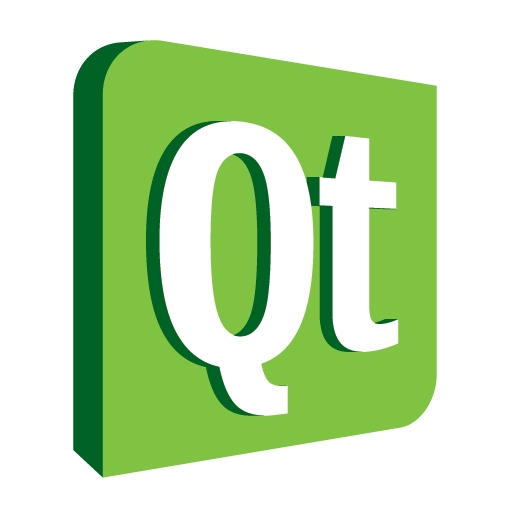
\includegraphics[height=2cm]{images/qt-logo} \\ http://qt.nokia.com}
  }

\usepackage{fontspec}
\usepackage{xunicode}

% set the default roman font
\setmainfont[Scale=0.9]{Arial}

% set the default sans font
\setsansfont[Scale=0.9]{Arial}

% set the default mono font
\setmonofont[Scale=0.8]{Liberation Mono}

% define new font families for main body, footnote, title
\newfontfamily\slidebodyfont{Arial}

\newfontfamily\slidefootnotefont{Arial}

\newfontfamily\slidetitlefont{Arial Bold}



% General course title
\title{Qt Essentials - OpenSource Edition}

\begin{document}

%%%%%%%%%%%%%%%%%%%%%%%%%%%%%%%%%%%%%%%%%%%%%%%%%%%%%%%%%%%%%%%%%%%%%%%%%%
%
% Copyright (c) 2008-2011, Nokia Corporation and/or its subsidiary(-ies).
% All rights reserved.
%
% This work, unless otherwise expressly stated, is licensed under a
% Creative Commons Attribution-ShareAlike 2.5.
%
% The full license document is available from
% http://creativecommons.org/licenses/by-sa/2.5/legalcode .
%
%%%%%%%%%%%%%%%%%%%%%%%%%%%%%%%%%%%%%%%%%%%%%%%%%%%%%%%%%%%%%%%%%%%%%%%%%%

% background for title page
\ifthenelse{\boolean{cc-license}}
{
  \setbeamertemplate{background canvas}{
\includegraphics[width=\paperwidth,height=\paperheight]{images/titlepage-background_cc}}
  \begin{slide}[plain]{0449}
    \titlepage
  \end{slide}

  % simple slide background
  \setbeamertemplate{background canvas}{
\includegraphics[width=\paperwidth,height=\paperheight]{images/background_cc}}
} % else
{
  \setbeamertemplate{background canvas}{
\includegraphics[width=\paperwidth,height=\paperheight]{images/titlepage-background}}
  \begin{slide}[plain]{0449}
    \titlepage
  \end{slide}

  % simple slide background
  \setbeamertemplate{background canvas}{
\includegraphics[width=\paperwidth,height=\paperheight]{images/background}}
}


\begin{slide}{1441}
  \frametitle{Part 1}
  \tableofcontents[part=1]
\end{slide}

\part{Part 1}
%%%%%%%%%%%%%%%%%%%%%%%%%%%%%%%%%%%%%%%%%%%%%%%%%%%%%%%%%%%%%%%%%%%%%%%%%%
%
% Copyright (c) 2008-2012, Nokia Corporation and/or its subsidiary(-ies).
% All rights reserved.
%
% This work, unless otherwise expressly stated, is licensed under a
% Creative Commons Attribution-ShareAlike 2.5.
%
% The full license document is available from
% http://creativecommons.org/licenses/by-sa/2.5/legalcode .
%
%%%%%%%%%%%%%%%%%%%%%%%%%%%%%%%%%%%%%%%%%%%%%%%%%%%%%%%%%%%%%%%%%%%%%%%%%%

\section{Graphics Effects}

%----------------------------------------------------------------------
\begin{slide}{1790}\frametitle{Objectives}

\vspace*{1em}
\begin{itemize}
\item Knowledge on how to create items with your own painting code
\item Use canvas with user interaction of animations
\item Create a complete particle system
  \begin{itemize}
  \item Specify the particles
  \item Provide speed, acceleration or other physics traits
  \end{itemize}
\item Use shaders to modify items rendering
  \begin{itemize}
  \item Fragment shaders for pixel manipulation
  \item Vertex shaders for shape manipulation
  \end{itemize}
\end{itemize}

\end{slide}

%----------------------------------------------------------------------
\begin{slide}{1791}\frametitle{Why use canvas, particles and shaders?}
\flushedImage{qml-graphics-effects/images/effects-showcase.png}

\begin{itemize}
\item Custom painting of components
\item Graphs and plots
\end{itemize}
\vspace*{0.5em}
\begin{itemize}
\item Complex visual effects
\item Simulate some physics during animations
\item Benefit as much as possible from the GPU
\end{itemize}

\demo{qml-graphics-effects/ex-canvas/piechart.qml}

\demo{qml-graphics-effects/ex-flickr/flickr.qml}
\end{slide}

%%%%%%%%%%%%%%%%%%%%%%%%%%%%%%%%%%%%%%%%%%%%%%%%%%%%%%%%%%%%%%%%%%%%%%%%%%
%
% Copyright (c) 2008-2012, Nokia Corporation and/or its subsidiary(-ies).
% All rights reserved.
%
% This work, unless otherwise expressly stated, is licensed under a
% Creative Commons Attribution-ShareAlike 2.5.
%
% The full license document is available from
% http://creativecommons.org/licenses/by-sa/2.5/legalcode .
%
%%%%%%%%%%%%%%%%%%%%%%%%%%%%%%%%%%%%%%%%%%%%%%%%%%%%%%%%%%%%%%%%%%%%%%%%%%

\subsection{Canvas}

%----------------------------------------------------------------------

\begin{slide}{1800}\frametitle{Canvas}

\begin{itemize}
\item \qic{class}{Canvas} is used to insert an element in which to paint
\item \qic{type}{onPaint} handler will contain the painting code
\item API somewhat similar to the old \qic{class}{QPainter} API
\item API compatible with the HTML5 Canvas API
  \begin{itemize}
  \item Need to request a \qic{class}{Context2D} instance first
  \end{itemize}
\item \qic{type}{requestPaint()} method to schedule repainting
\end{itemize}
\end{slide}

%----------------------------------------------------------------------

\begin{slide}{1801}\frametitle{Path Rendering}
\flushedImage{qml-graphics-effects/images/path-painting.png}

\inputqml{qml-graphics-effects/colorized/path-painting}

\demo{qml-graphics-effects/ex-canvas/path-painting.qml}
\end{slide}

%----------------------------------------------------------------------

\begin{slide}{1802}\frametitle{Scribble Area}
\inputqml{qml-graphics-effects/colorized/scribble-area}

\demo{qml-graphics-effects/ex-canvas/scribble-area.qml}
\end{slide}

%----------------------------------------------------------------------

\begin{slide}{1803}\frametitle{Lab: Screen Saver}
\centeredImage{qml-graphics-effects/images/screensaver.png}

Starting from the partial solution:

\begin{itemize}
\item Get the lines to be rendered
\item Have the points forming the lines animated
\end{itemize}

\lab{qml-graphics-effects/lab-screensaver/screensaver.qml}
\end{slide}


%%%%%%%%%%%%%%%%%%%%%%%%%%%%%%%%%%%%%%%%%%%%%%%%%%%%%%%%%%%%%%%%%%%%%%%%%%
%
% Copyright (c) 2008-2012, Nokia Corporation and/or its subsidiary(-ies).
% All rights reserved.
%
% This work, unless otherwise expressly stated, is licensed under a
% Creative Commons Attribution-ShareAlike 2.5.
%
% The full license document is available from
% http://creativecommons.org/licenses/by-sa/2.5/legalcode .
%
%%%%%%%%%%%%%%%%%%%%%%%%%%%%%%%%%%%%%%%%%%%%%%%%%%%%%%%%%%%%%%%%%%%%%%%%%%

\subsection{Particles}

%----------------------------------------------------------------------

\begin{slide}{1810}\frametitle{Particle System}

\begin{itemize}
\item A \qic{class}{ParticleSystem} requires
  \begin{itemize}
  \item at least a particles source
  \item the description of how particles look
  \end{itemize}
\vspace*{0.5em}
\item Particles sources are \qic{class}{Emitter} instances
  \begin{itemize}
  \item They emit the logical particles
  \item Provide initial attributes: \qic{type}{emitRate}, \qic{type}{lifeSpan}, \qic{type}{size}, \qic{type}{speed}, ...
  \item The flow can be controlled using \qic{type}{enabled}, \qic{type}{pulse()} and \qic{type}{burst()}
  \end{itemize}
\vspace*{0.5em}
\item Particle appearance is controlled by a \qic{class}{ParticlePainter} instance
  \begin{itemize}
  \item \qic{class}{ImageParticle} uses an image as \qic{type}{source}, it can be rotated, colorized, etc.
  \item \qic{class}{ItemParticle} uses an \qic{class}{Item} \qic{type}{delegate} to render particles
  \item \qic{class}{CustomParticle} uses shaders to render particles
  \end{itemize}
\end{itemize}

\end{slide}

%----------------------------------------------------------------------

\begin{slide}{1811}\frametitle{Christmas Lights}
\inputqml{qml-graphics-effects/colorized/christmas-lights}

\demo{qml-graphics-effects/ex-particles/christmas-lights.qml}

\vspace*{-20em}\hfill\image{qml-graphics-effects/images/christmas-lights.png}
\end{slide}

%----------------------------------------------------------------------

\begin{slide}{1812}\frametitle{Physics: Speed \& Acceleration}

\begin{itemize}
\item Both initial \qic{type}{speed} and \qic{type}{acceleration} are specified using a \qic{class}{Direction}
\vspace*{0.5em}
\item A \qic{class}{Direction} is a vector space of possible directions for a particle
  \begin{itemize}
  \item Value intervals are specified using \qic{type}{*Variation} properties
  \item Each particle gets a random vector of the vector space
  \end{itemize}
\vspace*{0.5em}
\item \qic{class}{Direction} is never used, it has subclasses
  \begin{itemize}
  \item \qic{class}{AngleDirection} for directions varying in \qic{type}{angle}
  \item \qic{class}{PointDirection} for directions varying in \qic{type}{x} and \qic{type}{y} components
  \item \qic{class}{TargetDirection} for directions toward a \qic{type}{targetItem}
  \item \qic{class}{CumulativeDirection} acts as a direction that sums the directions within it
  \end{itemize}
\end{itemize}

\end{slide}

%----------------------------------------------------------------------

\begin{slide}{1813}\frametitle{Explosion}
\inputqml{qml-graphics-effects/colorized/explosion}

\demo{qml-graphics-effects/ex-particles/explosion.qml}

\vspace*{-20em}\hfill\image{qml-graphics-effects/images/explosion.png}
\end{slide}

%----------------------------------------------------------------------

\begin{slide}{1814}\frametitle{Physics: Force fields}

\begin{itemize}
\item \qic{class}{Affector} instances can impact any attribute of the particles
  \begin{itemize}
  \item Behavior provided by \qic{type}{onAffectParticles}
  \item Gives access to all the \qic{type}{particles}
  \item \qic{type}{dt} is the time since last call (used to normalize to real time)
  \item Not recommended in high-volume particle systems (JS code being slower)
  \end{itemize}
\vspace*{0.5em}
\item Most common cases are covered with \qic{class}{Affector} subclasses
  \begin{itemize}
  \item \qic{class}{Attractor} attracts toward a point (magnetism, close object gravity)\linebreak\demo{qml-graphics-effects/ex-particles/explosion-implosion.qml}
  \item \qic{class}{Gravity} accelerates to a given vector (constant gravitational pull)
  \item \qic{class}{Friction} slows down proportionally to particles speed
  \item \qic{class}{Turbulence} provides fluid like forces based on a \qic{type}{noiseSource} image map
  \item \qic{class}{Wander} provides random particle perturbations
  \item ...
  \end{itemize}
\vspace*{0.5em}
\item The subclasses are C++ based and so much faster
\end{itemize}

\end{slide}

%----------------------------------------------------------------------

\begin{slide}{1815}\frametitle{Fountain}
\inputqml{qml-graphics-effects/colorized/fountain}

\demo{qml-graphics-effects/ex-particles/fountain.qml}

\vspace*{-10em}\hfill\image{qml-graphics-effects/images/fountain.png}
\end{slide}

%----------------------------------------------------------------------

\begin{slide}{1816}\frametitle{Lab: Screen Saver}
\centeredImage{qml-graphics-effects/images/makeitsnow.png}

Starting from the partial solution:

\begin{itemize}
\item Get the snow flakes to slowly fall
\item Make sure they're not all going exactly in the same direction/speed
\item Optionally: Get the snow flakes to rotate as they fall
\end{itemize}

\lab{qml-graphics-effects/lab-makeitsnow/makeitsnow.qml}
\end{slide}


%%%%%%%%%%%%%%%%%%%%%%%%%%%%%%%%%%%%%%%%%%%%%%%%%%%%%%%%%%%%%%%%%%%%%%%%%%
%
% Copyright (c) 2008-2012, Nokia Corporation and/or its subsidiary(-ies).
% All rights reserved.
%
% This work, unless otherwise expressly stated, is licensed under a
% Creative Commons Attribution-ShareAlike 2.5.
%
% The full license document is available from
% http://creativecommons.org/licenses/by-sa/2.5/legalcode .
%
%%%%%%%%%%%%%%%%%%%%%%%%%%%%%%%%%%%%%%%%%%%%%%%%%%%%%%%%%%%%%%%%%%%%%%%%%%

\subsection{Shaders}

%----------------------------------------------------------------------

\begin{slide}{1820}\frametitle{Shaders}

\begin{itemize}
\item A shader is a program used to calculate rendering effects on the GPU
\vspace*{1em}
\item Two types of shader are available in Qt Quick
  \begin{itemize}
  \item Fragment shaders
    \begin{itemize}
    \item Operate on each pixel
    \item Cannot be complex as it has no knowledge of the scene geometry
    \item Used for color manipulation, bump mapping, shadows, etc.
    \end{itemize}
  \item Vertex shaders
    \begin{itemize}
    \item Operate on each vertex
    \item Can change position, color and texture coordinate
    \item Cannot create new vertices
    \end{itemize}
  \end{itemize}
\item Their execution is heavily parallelized in the GPU pipeline
\item Extremely efficient
\item Written using OpenGL Shading Language (GLSL)
\end{itemize}

\end{slide}

%----------------------------------------------------------------------

\begin{slide}{1821}\frametitle{Fragment Shaders}

\begin{itemize}
\item \qic{class}{ShaderEffect} is a rectangle displaying the result of a shader program
\item The \qic{type}{fragmentShader} property is a string with the fragment shader code
\item Often such shaders use textures as inputs
\vspace*{1em}
\item \qic{class}{ShaderEffectSource} allows to render an item as a texture
\item \qic{type}{sourceItem} holds the \qic{class}{Item} to be rendered
\vspace*{1em}
\item Note that \qic{class}{ShaderEffectSource} is an invisible element aimed at consumption in \qic{class}{ShaderEffect} instances
\end{itemize}

\end{slide}

%----------------------------------------------------------------------

\begin{slide}{1822}\frametitle{Saturation Filter}
\inputqml{qml-graphics-effects/colorized/saturation-filter}

\demo{qml-graphics-effects/ex-shaders/saturation-filter.qml}

\vspace*{-20em}\hfill\image{qml-graphics-effects/images/saturation-filter.png}
\end{slide}

%----------------------------------------------------------------------

\begin{slide}{1823}\frametitle{Vertex Shaders}

\begin{itemize}
\item Works similarly to fragment shaders
\item Use the \qic{type}{vertexShader} property for the vertex shader code
\item Pay attention to the \qic{type}{mesh} property
  \begin{itemize}
  \item Specifies the number of vertices of the \qic{class}{ShaderEffect} element
  \item It must be fine enough to resolve the transformation
  \end{itemize}
\end{itemize}

\end{slide}

%----------------------------------------------------------------------

\begin{slide}{1824}\frametitle{Flag}
\inputqml{qml-graphics-effects/colorized/flag}

\demo{qml-graphics-effects/ex-shaders/flag.qml}

\vspace*{-20em}\hfill\image{qml-graphics-effects/images/flag.png}
\end{slide}

%----------------------------------------------------------------------

\begin{slide}{1825}\frametitle{Chaining Shaders}

\begin{itemize}
\item \qic{class}{ShaderEffectSource} can have any \qic{class}{Item} as \qic{type}{sourceItem}
\item Even a \qic{class}{ShaderEffect}!
\item Allows to create complex effects by chaining shader programs
\end{itemize}

\end{slide}

%----------------------------------------------------------------------

\begin{slide}{1826}\frametitle{Drop Shadow}
\centeredImage{qml-graphics-effects/images/drop-shadow.png}

\vspace*{2em}
A drop shadow is a combination of:

\begin{itemize}
\item A blur operation
\item A darkening of the result of the blur
\item A composition of the original on top of the created shadow with an offset
\end{itemize}

\demo{qml-graphics-effects/ex-shaders/drop-shadow.qml}
\end{slide}

%----------------------------------------------------------------------

\begin{slide}{1827}\frametitle{QtGraphicalEffects}

\begin{itemize}
\item New module providing reusable elements with premade shaders
\item Fairly extensive list of effects
  \begin{itemize}
  \item Colorize
  \item Gradients
  \item Blurs
  \item Gamma and levels adjustments
  \item Drop shadows
  \item Glows
  \item ...
  \end{itemize}
\end{itemize}

\demo{qml-graphics-effects/ex-shaders/drop-shadow2.qml}
\end{slide}

%----------------------------------------------------------------------

\begin{slide}{1828}\frametitle{Shaders and Particles}

\begin{itemize}
\item Everything about the particle systems is still valid
\item Allows for less CPU intensive particle rendering

\vspace*{1em}

\item Use \qic{class}{CustomParticle} instead of \qic{class}{ImageParticle}
\item Use the \qic{type}{vertexShader} and \qic{type}{fragmentShader} properties
\end{itemize}

\vspace*{2em}

\demo{qml-graphics-effects/ex-shaders/fountain-shaders.qml}
\end{slide}

%----------------------------------------------------------------------

\begin{slide}{1829}\frametitle{Lab: Dissolve Effect}
\centeredImage{qml-graphics-effects/images/dissolve.png}

Starting from the partial solution:

\begin{itemize}
\item Create an alpha gradient effect
\item Animate it so the item fades out from top to bottom and back in again
\end{itemize}

\lab{qml-graphics-effects/lab-dissolve/dissolve.qml}
\end{slide}




%%%%%%%%%%%%%%%%%%%%%%%%%%%%%%%%%%%%%%%%%%%%%%%%%%%%%%%%%%%%%%%%%%%%%%%%%%
%
% Copyright (c) 2008-2012, Nokia Corporation and/or its subsidiary(-ies).
% All rights reserved.
%
% This work, unless otherwise expressly stated, is licensed under a
% Creative Commons Attribution-ShareAlike 2.5.
%
% The full license document is available from
% http://creativecommons.org/licenses/by-sa/2.5/legalcode .
%
%%%%%%%%%%%%%%%%%%%%%%%%%%%%%%%%%%%%%%%%%%%%%%%%%%%%%%%%%%%%%%%%%%%%%%%%%%

\section{Graphics Effects}

%----------------------------------------------------------------------
\begin{slide}{1790}\frametitle{Objectives}

\vspace*{1em}
\begin{itemize}
\item Knowledge on how to create items with your own painting code
\item Use canvas with user interaction of animations
\item Create a complete particle system
  \begin{itemize}
  \item Specify the particles
  \item Provide speed, acceleration or other physics traits
  \end{itemize}
\item Use shaders to modify items rendering
  \begin{itemize}
  \item Fragment shaders for pixel manipulation
  \item Vertex shaders for shape manipulation
  \end{itemize}
\end{itemize}

\end{slide}

%----------------------------------------------------------------------
\begin{slide}{1791}\frametitle{Why use canvas, particles and shaders?}
\flushedImage{qml-graphics-effects/images/effects-showcase.png}

\begin{itemize}
\item Custom painting of components
\item Graphs and plots
\end{itemize}
\vspace*{0.5em}
\begin{itemize}
\item Complex visual effects
\item Simulate some physics during animations
\item Benefit as much as possible from the GPU
\end{itemize}

\demo{qml-graphics-effects/ex-canvas/piechart.qml}

\demo{qml-graphics-effects/ex-flickr/flickr.qml}
\end{slide}

%%%%%%%%%%%%%%%%%%%%%%%%%%%%%%%%%%%%%%%%%%%%%%%%%%%%%%%%%%%%%%%%%%%%%%%%%%
%
% Copyright (c) 2008-2012, Nokia Corporation and/or its subsidiary(-ies).
% All rights reserved.
%
% This work, unless otherwise expressly stated, is licensed under a
% Creative Commons Attribution-ShareAlike 2.5.
%
% The full license document is available from
% http://creativecommons.org/licenses/by-sa/2.5/legalcode .
%
%%%%%%%%%%%%%%%%%%%%%%%%%%%%%%%%%%%%%%%%%%%%%%%%%%%%%%%%%%%%%%%%%%%%%%%%%%

\subsection{Canvas}

%----------------------------------------------------------------------

\begin{slide}{1800}\frametitle{Canvas}

\begin{itemize}
\item \qic{class}{Canvas} is used to insert an element in which to paint
\item \qic{type}{onPaint} handler will contain the painting code
\item API somewhat similar to the old \qic{class}{QPainter} API
\item API compatible with the HTML5 Canvas API
  \begin{itemize}
  \item Need to request a \qic{class}{Context2D} instance first
  \end{itemize}
\item \qic{type}{requestPaint()} method to schedule repainting
\end{itemize}
\end{slide}

%----------------------------------------------------------------------

\begin{slide}{1801}\frametitle{Path Rendering}
\flushedImage{qml-graphics-effects/images/path-painting.png}

\inputqml{qml-graphics-effects/colorized/path-painting}

\demo{qml-graphics-effects/ex-canvas/path-painting.qml}
\end{slide}

%----------------------------------------------------------------------

\begin{slide}{1802}\frametitle{Scribble Area}
\inputqml{qml-graphics-effects/colorized/scribble-area}

\demo{qml-graphics-effects/ex-canvas/scribble-area.qml}
\end{slide}

%----------------------------------------------------------------------

\begin{slide}{1803}\frametitle{Lab: Screen Saver}
\centeredImage{qml-graphics-effects/images/screensaver.png}

Starting from the partial solution:

\begin{itemize}
\item Get the lines to be rendered
\item Have the points forming the lines animated
\end{itemize}

\lab{qml-graphics-effects/lab-screensaver/screensaver.qml}
\end{slide}


%%%%%%%%%%%%%%%%%%%%%%%%%%%%%%%%%%%%%%%%%%%%%%%%%%%%%%%%%%%%%%%%%%%%%%%%%%
%
% Copyright (c) 2008-2012, Nokia Corporation and/or its subsidiary(-ies).
% All rights reserved.
%
% This work, unless otherwise expressly stated, is licensed under a
% Creative Commons Attribution-ShareAlike 2.5.
%
% The full license document is available from
% http://creativecommons.org/licenses/by-sa/2.5/legalcode .
%
%%%%%%%%%%%%%%%%%%%%%%%%%%%%%%%%%%%%%%%%%%%%%%%%%%%%%%%%%%%%%%%%%%%%%%%%%%

\subsection{Particles}

%----------------------------------------------------------------------

\begin{slide}{1810}\frametitle{Particle System}

\begin{itemize}
\item A \qic{class}{ParticleSystem} requires
  \begin{itemize}
  \item at least a particles source
  \item the description of how particles look
  \end{itemize}
\vspace*{0.5em}
\item Particles sources are \qic{class}{Emitter} instances
  \begin{itemize}
  \item They emit the logical particles
  \item Provide initial attributes: \qic{type}{emitRate}, \qic{type}{lifeSpan}, \qic{type}{size}, \qic{type}{speed}, ...
  \item The flow can be controlled using \qic{type}{enabled}, \qic{type}{pulse()} and \qic{type}{burst()}
  \end{itemize}
\vspace*{0.5em}
\item Particle appearance is controlled by a \qic{class}{ParticlePainter} instance
  \begin{itemize}
  \item \qic{class}{ImageParticle} uses an image as \qic{type}{source}, it can be rotated, colorized, etc.
  \item \qic{class}{ItemParticle} uses an \qic{class}{Item} \qic{type}{delegate} to render particles
  \item \qic{class}{CustomParticle} uses shaders to render particles
  \end{itemize}
\end{itemize}

\end{slide}

%----------------------------------------------------------------------

\begin{slide}{1811}\frametitle{Christmas Lights}
\inputqml{qml-graphics-effects/colorized/christmas-lights}

\demo{qml-graphics-effects/ex-particles/christmas-lights.qml}

\vspace*{-20em}\hfill\image{qml-graphics-effects/images/christmas-lights.png}
\end{slide}

%----------------------------------------------------------------------

\begin{slide}{1812}\frametitle{Physics: Speed \& Acceleration}

\begin{itemize}
\item Both initial \qic{type}{speed} and \qic{type}{acceleration} are specified using a \qic{class}{Direction}
\vspace*{0.5em}
\item A \qic{class}{Direction} is a vector space of possible directions for a particle
  \begin{itemize}
  \item Value intervals are specified using \qic{type}{*Variation} properties
  \item Each particle gets a random vector of the vector space
  \end{itemize}
\vspace*{0.5em}
\item \qic{class}{Direction} is never used, it has subclasses
  \begin{itemize}
  \item \qic{class}{AngleDirection} for directions varying in \qic{type}{angle}
  \item \qic{class}{PointDirection} for directions varying in \qic{type}{x} and \qic{type}{y} components
  \item \qic{class}{TargetDirection} for directions toward a \qic{type}{targetItem}
  \item \qic{class}{CumulativeDirection} acts as a direction that sums the directions within it
  \end{itemize}
\end{itemize}

\end{slide}

%----------------------------------------------------------------------

\begin{slide}{1813}\frametitle{Explosion}
\inputqml{qml-graphics-effects/colorized/explosion}

\demo{qml-graphics-effects/ex-particles/explosion.qml}

\vspace*{-20em}\hfill\image{qml-graphics-effects/images/explosion.png}
\end{slide}

%----------------------------------------------------------------------

\begin{slide}{1814}\frametitle{Physics: Force fields}

\begin{itemize}
\item \qic{class}{Affector} instances can impact any attribute of the particles
  \begin{itemize}
  \item Behavior provided by \qic{type}{onAffectParticles}
  \item Gives access to all the \qic{type}{particles}
  \item \qic{type}{dt} is the time since last call (used to normalize to real time)
  \item Not recommended in high-volume particle systems (JS code being slower)
  \end{itemize}
\vspace*{0.5em}
\item Most common cases are covered with \qic{class}{Affector} subclasses
  \begin{itemize}
  \item \qic{class}{Attractor} attracts toward a point (magnetism, close object gravity)\linebreak\demo{qml-graphics-effects/ex-particles/explosion-implosion.qml}
  \item \qic{class}{Gravity} accelerates to a given vector (constant gravitational pull)
  \item \qic{class}{Friction} slows down proportionally to particles speed
  \item \qic{class}{Turbulence} provides fluid like forces based on a \qic{type}{noiseSource} image map
  \item \qic{class}{Wander} provides random particle perturbations
  \item ...
  \end{itemize}
\vspace*{0.5em}
\item The subclasses are C++ based and so much faster
\end{itemize}

\end{slide}

%----------------------------------------------------------------------

\begin{slide}{1815}\frametitle{Fountain}
\inputqml{qml-graphics-effects/colorized/fountain}

\demo{qml-graphics-effects/ex-particles/fountain.qml}

\vspace*{-10em}\hfill\image{qml-graphics-effects/images/fountain.png}
\end{slide}

%----------------------------------------------------------------------

\begin{slide}{1816}\frametitle{Lab: Screen Saver}
\centeredImage{qml-graphics-effects/images/makeitsnow.png}

Starting from the partial solution:

\begin{itemize}
\item Get the snow flakes to slowly fall
\item Make sure they're not all going exactly in the same direction/speed
\item Optionally: Get the snow flakes to rotate as they fall
\end{itemize}

\lab{qml-graphics-effects/lab-makeitsnow/makeitsnow.qml}
\end{slide}


%%%%%%%%%%%%%%%%%%%%%%%%%%%%%%%%%%%%%%%%%%%%%%%%%%%%%%%%%%%%%%%%%%%%%%%%%%
%
% Copyright (c) 2008-2012, Nokia Corporation and/or its subsidiary(-ies).
% All rights reserved.
%
% This work, unless otherwise expressly stated, is licensed under a
% Creative Commons Attribution-ShareAlike 2.5.
%
% The full license document is available from
% http://creativecommons.org/licenses/by-sa/2.5/legalcode .
%
%%%%%%%%%%%%%%%%%%%%%%%%%%%%%%%%%%%%%%%%%%%%%%%%%%%%%%%%%%%%%%%%%%%%%%%%%%

\subsection{Shaders}

%----------------------------------------------------------------------

\begin{slide}{1820}\frametitle{Shaders}

\begin{itemize}
\item A shader is a program used to calculate rendering effects on the GPU
\vspace*{1em}
\item Two types of shader are available in Qt Quick
  \begin{itemize}
  \item Fragment shaders
    \begin{itemize}
    \item Operate on each pixel
    \item Cannot be complex as it has no knowledge of the scene geometry
    \item Used for color manipulation, bump mapping, shadows, etc.
    \end{itemize}
  \item Vertex shaders
    \begin{itemize}
    \item Operate on each vertex
    \item Can change position, color and texture coordinate
    \item Cannot create new vertices
    \end{itemize}
  \end{itemize}
\item Their execution is heavily parallelized in the GPU pipeline
\item Extremely efficient
\item Written using OpenGL Shading Language (GLSL)
\end{itemize}

\end{slide}

%----------------------------------------------------------------------

\begin{slide}{1821}\frametitle{Fragment Shaders}

\begin{itemize}
\item \qic{class}{ShaderEffect} is a rectangle displaying the result of a shader program
\item The \qic{type}{fragmentShader} property is a string with the fragment shader code
\item Often such shaders use textures as inputs
\vspace*{1em}
\item \qic{class}{ShaderEffectSource} allows to render an item as a texture
\item \qic{type}{sourceItem} holds the \qic{class}{Item} to be rendered
\vspace*{1em}
\item Note that \qic{class}{ShaderEffectSource} is an invisible element aimed at consumption in \qic{class}{ShaderEffect} instances
\end{itemize}

\end{slide}

%----------------------------------------------------------------------

\begin{slide}{1822}\frametitle{Saturation Filter}
\inputqml{qml-graphics-effects/colorized/saturation-filter}

\demo{qml-graphics-effects/ex-shaders/saturation-filter.qml}

\vspace*{-20em}\hfill\image{qml-graphics-effects/images/saturation-filter.png}
\end{slide}

%----------------------------------------------------------------------

\begin{slide}{1823}\frametitle{Vertex Shaders}

\begin{itemize}
\item Works similarly to fragment shaders
\item Use the \qic{type}{vertexShader} property for the vertex shader code
\item Pay attention to the \qic{type}{mesh} property
  \begin{itemize}
  \item Specifies the number of vertices of the \qic{class}{ShaderEffect} element
  \item It must be fine enough to resolve the transformation
  \end{itemize}
\end{itemize}

\end{slide}

%----------------------------------------------------------------------

\begin{slide}{1824}\frametitle{Flag}
\inputqml{qml-graphics-effects/colorized/flag}

\demo{qml-graphics-effects/ex-shaders/flag.qml}

\vspace*{-20em}\hfill\image{qml-graphics-effects/images/flag.png}
\end{slide}

%----------------------------------------------------------------------

\begin{slide}{1825}\frametitle{Chaining Shaders}

\begin{itemize}
\item \qic{class}{ShaderEffectSource} can have any \qic{class}{Item} as \qic{type}{sourceItem}
\item Even a \qic{class}{ShaderEffect}!
\item Allows to create complex effects by chaining shader programs
\end{itemize}

\end{slide}

%----------------------------------------------------------------------

\begin{slide}{1826}\frametitle{Drop Shadow}
\centeredImage{qml-graphics-effects/images/drop-shadow.png}

\vspace*{2em}
A drop shadow is a combination of:

\begin{itemize}
\item A blur operation
\item A darkening of the result of the blur
\item A composition of the original on top of the created shadow with an offset
\end{itemize}

\demo{qml-graphics-effects/ex-shaders/drop-shadow.qml}
\end{slide}

%----------------------------------------------------------------------

\begin{slide}{1827}\frametitle{QtGraphicalEffects}

\begin{itemize}
\item New module providing reusable elements with premade shaders
\item Fairly extensive list of effects
  \begin{itemize}
  \item Colorize
  \item Gradients
  \item Blurs
  \item Gamma and levels adjustments
  \item Drop shadows
  \item Glows
  \item ...
  \end{itemize}
\end{itemize}

\demo{qml-graphics-effects/ex-shaders/drop-shadow2.qml}
\end{slide}

%----------------------------------------------------------------------

\begin{slide}{1828}\frametitle{Shaders and Particles}

\begin{itemize}
\item Everything about the particle systems is still valid
\item Allows for less CPU intensive particle rendering

\vspace*{1em}

\item Use \qic{class}{CustomParticle} instead of \qic{class}{ImageParticle}
\item Use the \qic{type}{vertexShader} and \qic{type}{fragmentShader} properties
\end{itemize}

\vspace*{2em}

\demo{qml-graphics-effects/ex-shaders/fountain-shaders.qml}
\end{slide}

%----------------------------------------------------------------------

\begin{slide}{1829}\frametitle{Lab: Dissolve Effect}
\centeredImage{qml-graphics-effects/images/dissolve.png}

Starting from the partial solution:

\begin{itemize}
\item Create an alpha gradient effect
\item Animate it so the item fades out from top to bottom and back in again
\end{itemize}

\lab{qml-graphics-effects/lab-dissolve/dissolve.qml}
\end{slide}




%%%%%%%%%%%%%%%%%%%%%%%%%%%%%%%%%%%%%%%%%%%%%%%%%%%%%%%%%%%%%%%%%%%%%%%%%%
%
% Copyright (c) 2008-2012, Nokia Corporation and/or its subsidiary(-ies).
% All rights reserved.
%
% This work, unless otherwise expressly stated, is licensed under a
% Creative Commons Attribution-ShareAlike 2.5.
%
% The full license document is available from
% http://creativecommons.org/licenses/by-sa/2.5/legalcode .
%
%%%%%%%%%%%%%%%%%%%%%%%%%%%%%%%%%%%%%%%%%%%%%%%%%%%%%%%%%%%%%%%%%%%%%%%%%%

\section{Graphics Effects}

%----------------------------------------------------------------------
\begin{slide}{1790}\frametitle{Objectives}

\vspace*{1em}
\begin{itemize}
\item Knowledge on how to create items with your own painting code
\item Use canvas with user interaction of animations
\item Create a complete particle system
  \begin{itemize}
  \item Specify the particles
  \item Provide speed, acceleration or other physics traits
  \end{itemize}
\item Use shaders to modify items rendering
  \begin{itemize}
  \item Fragment shaders for pixel manipulation
  \item Vertex shaders for shape manipulation
  \end{itemize}
\end{itemize}

\end{slide}

%----------------------------------------------------------------------
\begin{slide}{1791}\frametitle{Why use canvas, particles and shaders?}
\flushedImage{qml-graphics-effects/images/effects-showcase.png}

\begin{itemize}
\item Custom painting of components
\item Graphs and plots
\end{itemize}
\vspace*{0.5em}
\begin{itemize}
\item Complex visual effects
\item Simulate some physics during animations
\item Benefit as much as possible from the GPU
\end{itemize}

\demo{qml-graphics-effects/ex-canvas/piechart.qml}

\demo{qml-graphics-effects/ex-flickr/flickr.qml}
\end{slide}

%%%%%%%%%%%%%%%%%%%%%%%%%%%%%%%%%%%%%%%%%%%%%%%%%%%%%%%%%%%%%%%%%%%%%%%%%%
%
% Copyright (c) 2008-2012, Nokia Corporation and/or its subsidiary(-ies).
% All rights reserved.
%
% This work, unless otherwise expressly stated, is licensed under a
% Creative Commons Attribution-ShareAlike 2.5.
%
% The full license document is available from
% http://creativecommons.org/licenses/by-sa/2.5/legalcode .
%
%%%%%%%%%%%%%%%%%%%%%%%%%%%%%%%%%%%%%%%%%%%%%%%%%%%%%%%%%%%%%%%%%%%%%%%%%%

\subsection{Canvas}

%----------------------------------------------------------------------

\begin{slide}{1800}\frametitle{Canvas}

\begin{itemize}
\item \qic{class}{Canvas} is used to insert an element in which to paint
\item \qic{type}{onPaint} handler will contain the painting code
\item API somewhat similar to the old \qic{class}{QPainter} API
\item API compatible with the HTML5 Canvas API
  \begin{itemize}
  \item Need to request a \qic{class}{Context2D} instance first
  \end{itemize}
\item \qic{type}{requestPaint()} method to schedule repainting
\end{itemize}
\end{slide}

%----------------------------------------------------------------------

\begin{slide}{1801}\frametitle{Path Rendering}
\flushedImage{qml-graphics-effects/images/path-painting.png}

\inputqml{qml-graphics-effects/colorized/path-painting}

\demo{qml-graphics-effects/ex-canvas/path-painting.qml}
\end{slide}

%----------------------------------------------------------------------

\begin{slide}{1802}\frametitle{Scribble Area}
\inputqml{qml-graphics-effects/colorized/scribble-area}

\demo{qml-graphics-effects/ex-canvas/scribble-area.qml}
\end{slide}

%----------------------------------------------------------------------

\begin{slide}{1803}\frametitle{Lab: Screen Saver}
\centeredImage{qml-graphics-effects/images/screensaver.png}

Starting from the partial solution:

\begin{itemize}
\item Get the lines to be rendered
\item Have the points forming the lines animated
\end{itemize}

\lab{qml-graphics-effects/lab-screensaver/screensaver.qml}
\end{slide}


%%%%%%%%%%%%%%%%%%%%%%%%%%%%%%%%%%%%%%%%%%%%%%%%%%%%%%%%%%%%%%%%%%%%%%%%%%
%
% Copyright (c) 2008-2012, Nokia Corporation and/or its subsidiary(-ies).
% All rights reserved.
%
% This work, unless otherwise expressly stated, is licensed under a
% Creative Commons Attribution-ShareAlike 2.5.
%
% The full license document is available from
% http://creativecommons.org/licenses/by-sa/2.5/legalcode .
%
%%%%%%%%%%%%%%%%%%%%%%%%%%%%%%%%%%%%%%%%%%%%%%%%%%%%%%%%%%%%%%%%%%%%%%%%%%

\subsection{Particles}

%----------------------------------------------------------------------

\begin{slide}{1810}\frametitle{Particle System}

\begin{itemize}
\item A \qic{class}{ParticleSystem} requires
  \begin{itemize}
  \item at least a particles source
  \item the description of how particles look
  \end{itemize}
\vspace*{0.5em}
\item Particles sources are \qic{class}{Emitter} instances
  \begin{itemize}
  \item They emit the logical particles
  \item Provide initial attributes: \qic{type}{emitRate}, \qic{type}{lifeSpan}, \qic{type}{size}, \qic{type}{speed}, ...
  \item The flow can be controlled using \qic{type}{enabled}, \qic{type}{pulse()} and \qic{type}{burst()}
  \end{itemize}
\vspace*{0.5em}
\item Particle appearance is controlled by a \qic{class}{ParticlePainter} instance
  \begin{itemize}
  \item \qic{class}{ImageParticle} uses an image as \qic{type}{source}, it can be rotated, colorized, etc.
  \item \qic{class}{ItemParticle} uses an \qic{class}{Item} \qic{type}{delegate} to render particles
  \item \qic{class}{CustomParticle} uses shaders to render particles
  \end{itemize}
\end{itemize}

\end{slide}

%----------------------------------------------------------------------

\begin{slide}{1811}\frametitle{Christmas Lights}
\inputqml{qml-graphics-effects/colorized/christmas-lights}

\demo{qml-graphics-effects/ex-particles/christmas-lights.qml}

\vspace*{-20em}\hfill\image{qml-graphics-effects/images/christmas-lights.png}
\end{slide}

%----------------------------------------------------------------------

\begin{slide}{1812}\frametitle{Physics: Speed \& Acceleration}

\begin{itemize}
\item Both initial \qic{type}{speed} and \qic{type}{acceleration} are specified using a \qic{class}{Direction}
\vspace*{0.5em}
\item A \qic{class}{Direction} is a vector space of possible directions for a particle
  \begin{itemize}
  \item Value intervals are specified using \qic{type}{*Variation} properties
  \item Each particle gets a random vector of the vector space
  \end{itemize}
\vspace*{0.5em}
\item \qic{class}{Direction} is never used, it has subclasses
  \begin{itemize}
  \item \qic{class}{AngleDirection} for directions varying in \qic{type}{angle}
  \item \qic{class}{PointDirection} for directions varying in \qic{type}{x} and \qic{type}{y} components
  \item \qic{class}{TargetDirection} for directions toward a \qic{type}{targetItem}
  \item \qic{class}{CumulativeDirection} acts as a direction that sums the directions within it
  \end{itemize}
\end{itemize}

\end{slide}

%----------------------------------------------------------------------

\begin{slide}{1813}\frametitle{Explosion}
\inputqml{qml-graphics-effects/colorized/explosion}

\demo{qml-graphics-effects/ex-particles/explosion.qml}

\vspace*{-20em}\hfill\image{qml-graphics-effects/images/explosion.png}
\end{slide}

%----------------------------------------------------------------------

\begin{slide}{1814}\frametitle{Physics: Force fields}

\begin{itemize}
\item \qic{class}{Affector} instances can impact any attribute of the particles
  \begin{itemize}
  \item Behavior provided by \qic{type}{onAffectParticles}
  \item Gives access to all the \qic{type}{particles}
  \item \qic{type}{dt} is the time since last call (used to normalize to real time)
  \item Not recommended in high-volume particle systems (JS code being slower)
  \end{itemize}
\vspace*{0.5em}
\item Most common cases are covered with \qic{class}{Affector} subclasses
  \begin{itemize}
  \item \qic{class}{Attractor} attracts toward a point (magnetism, close object gravity)\linebreak\demo{qml-graphics-effects/ex-particles/explosion-implosion.qml}
  \item \qic{class}{Gravity} accelerates to a given vector (constant gravitational pull)
  \item \qic{class}{Friction} slows down proportionally to particles speed
  \item \qic{class}{Turbulence} provides fluid like forces based on a \qic{type}{noiseSource} image map
  \item \qic{class}{Wander} provides random particle perturbations
  \item ...
  \end{itemize}
\vspace*{0.5em}
\item The subclasses are C++ based and so much faster
\end{itemize}

\end{slide}

%----------------------------------------------------------------------

\begin{slide}{1815}\frametitle{Fountain}
\inputqml{qml-graphics-effects/colorized/fountain}

\demo{qml-graphics-effects/ex-particles/fountain.qml}

\vspace*{-10em}\hfill\image{qml-graphics-effects/images/fountain.png}
\end{slide}

%----------------------------------------------------------------------

\begin{slide}{1816}\frametitle{Lab: Screen Saver}
\centeredImage{qml-graphics-effects/images/makeitsnow.png}

Starting from the partial solution:

\begin{itemize}
\item Get the snow flakes to slowly fall
\item Make sure they're not all going exactly in the same direction/speed
\item Optionally: Get the snow flakes to rotate as they fall
\end{itemize}

\lab{qml-graphics-effects/lab-makeitsnow/makeitsnow.qml}
\end{slide}


%%%%%%%%%%%%%%%%%%%%%%%%%%%%%%%%%%%%%%%%%%%%%%%%%%%%%%%%%%%%%%%%%%%%%%%%%%
%
% Copyright (c) 2008-2012, Nokia Corporation and/or its subsidiary(-ies).
% All rights reserved.
%
% This work, unless otherwise expressly stated, is licensed under a
% Creative Commons Attribution-ShareAlike 2.5.
%
% The full license document is available from
% http://creativecommons.org/licenses/by-sa/2.5/legalcode .
%
%%%%%%%%%%%%%%%%%%%%%%%%%%%%%%%%%%%%%%%%%%%%%%%%%%%%%%%%%%%%%%%%%%%%%%%%%%

\subsection{Shaders}

%----------------------------------------------------------------------

\begin{slide}{1820}\frametitle{Shaders}

\begin{itemize}
\item A shader is a program used to calculate rendering effects on the GPU
\vspace*{1em}
\item Two types of shader are available in Qt Quick
  \begin{itemize}
  \item Fragment shaders
    \begin{itemize}
    \item Operate on each pixel
    \item Cannot be complex as it has no knowledge of the scene geometry
    \item Used for color manipulation, bump mapping, shadows, etc.
    \end{itemize}
  \item Vertex shaders
    \begin{itemize}
    \item Operate on each vertex
    \item Can change position, color and texture coordinate
    \item Cannot create new vertices
    \end{itemize}
  \end{itemize}
\item Their execution is heavily parallelized in the GPU pipeline
\item Extremely efficient
\item Written using OpenGL Shading Language (GLSL)
\end{itemize}

\end{slide}

%----------------------------------------------------------------------

\begin{slide}{1821}\frametitle{Fragment Shaders}

\begin{itemize}
\item \qic{class}{ShaderEffect} is a rectangle displaying the result of a shader program
\item The \qic{type}{fragmentShader} property is a string with the fragment shader code
\item Often such shaders use textures as inputs
\vspace*{1em}
\item \qic{class}{ShaderEffectSource} allows to render an item as a texture
\item \qic{type}{sourceItem} holds the \qic{class}{Item} to be rendered
\vspace*{1em}
\item Note that \qic{class}{ShaderEffectSource} is an invisible element aimed at consumption in \qic{class}{ShaderEffect} instances
\end{itemize}

\end{slide}

%----------------------------------------------------------------------

\begin{slide}{1822}\frametitle{Saturation Filter}
\inputqml{qml-graphics-effects/colorized/saturation-filter}

\demo{qml-graphics-effects/ex-shaders/saturation-filter.qml}

\vspace*{-20em}\hfill\image{qml-graphics-effects/images/saturation-filter.png}
\end{slide}

%----------------------------------------------------------------------

\begin{slide}{1823}\frametitle{Vertex Shaders}

\begin{itemize}
\item Works similarly to fragment shaders
\item Use the \qic{type}{vertexShader} property for the vertex shader code
\item Pay attention to the \qic{type}{mesh} property
  \begin{itemize}
  \item Specifies the number of vertices of the \qic{class}{ShaderEffect} element
  \item It must be fine enough to resolve the transformation
  \end{itemize}
\end{itemize}

\end{slide}

%----------------------------------------------------------------------

\begin{slide}{1824}\frametitle{Flag}
\inputqml{qml-graphics-effects/colorized/flag}

\demo{qml-graphics-effects/ex-shaders/flag.qml}

\vspace*{-20em}\hfill\image{qml-graphics-effects/images/flag.png}
\end{slide}

%----------------------------------------------------------------------

\begin{slide}{1825}\frametitle{Chaining Shaders}

\begin{itemize}
\item \qic{class}{ShaderEffectSource} can have any \qic{class}{Item} as \qic{type}{sourceItem}
\item Even a \qic{class}{ShaderEffect}!
\item Allows to create complex effects by chaining shader programs
\end{itemize}

\end{slide}

%----------------------------------------------------------------------

\begin{slide}{1826}\frametitle{Drop Shadow}
\centeredImage{qml-graphics-effects/images/drop-shadow.png}

\vspace*{2em}
A drop shadow is a combination of:

\begin{itemize}
\item A blur operation
\item A darkening of the result of the blur
\item A composition of the original on top of the created shadow with an offset
\end{itemize}

\demo{qml-graphics-effects/ex-shaders/drop-shadow.qml}
\end{slide}

%----------------------------------------------------------------------

\begin{slide}{1827}\frametitle{QtGraphicalEffects}

\begin{itemize}
\item New module providing reusable elements with premade shaders
\item Fairly extensive list of effects
  \begin{itemize}
  \item Colorize
  \item Gradients
  \item Blurs
  \item Gamma and levels adjustments
  \item Drop shadows
  \item Glows
  \item ...
  \end{itemize}
\end{itemize}

\demo{qml-graphics-effects/ex-shaders/drop-shadow2.qml}
\end{slide}

%----------------------------------------------------------------------

\begin{slide}{1828}\frametitle{Shaders and Particles}

\begin{itemize}
\item Everything about the particle systems is still valid
\item Allows for less CPU intensive particle rendering

\vspace*{1em}

\item Use \qic{class}{CustomParticle} instead of \qic{class}{ImageParticle}
\item Use the \qic{type}{vertexShader} and \qic{type}{fragmentShader} properties
\end{itemize}

\vspace*{2em}

\demo{qml-graphics-effects/ex-shaders/fountain-shaders.qml}
\end{slide}

%----------------------------------------------------------------------

\begin{slide}{1829}\frametitle{Lab: Dissolve Effect}
\centeredImage{qml-graphics-effects/images/dissolve.png}

Starting from the partial solution:

\begin{itemize}
\item Create an alpha gradient effect
\item Animate it so the item fades out from top to bottom and back in again
\end{itemize}

\lab{qml-graphics-effects/lab-dissolve/dissolve.qml}
\end{slide}





\part{Part 2}
%%%%%%%%%%%%%%%%%%%%%%%%%%%%%%%%%%%%%%%%%%%%%%%%%%%%%%%%%%%%%%%%%%%%%%%%%%
%
% Copyright (c) 2008-2012, Nokia Corporation and/or its subsidiary(-ies).
% All rights reserved.
%
% This work, unless otherwise expressly stated, is licensed under a
% Creative Commons Attribution-ShareAlike 2.5.
%
% The full license document is available from
% http://creativecommons.org/licenses/by-sa/2.5/legalcode .
%
%%%%%%%%%%%%%%%%%%%%%%%%%%%%%%%%%%%%%%%%%%%%%%%%%%%%%%%%%%%%%%%%%%%%%%%%%%

\section{Graphics Effects}

%----------------------------------------------------------------------
\begin{slide}{1790}\frametitle{Objectives}

\vspace*{1em}
\begin{itemize}
\item Knowledge on how to create items with your own painting code
\item Use canvas with user interaction of animations
\item Create a complete particle system
  \begin{itemize}
  \item Specify the particles
  \item Provide speed, acceleration or other physics traits
  \end{itemize}
\item Use shaders to modify items rendering
  \begin{itemize}
  \item Fragment shaders for pixel manipulation
  \item Vertex shaders for shape manipulation
  \end{itemize}
\end{itemize}

\end{slide}

%----------------------------------------------------------------------
\begin{slide}{1791}\frametitle{Why use canvas, particles and shaders?}
\flushedImage{qml-graphics-effects/images/effects-showcase.png}

\begin{itemize}
\item Custom painting of components
\item Graphs and plots
\end{itemize}
\vspace*{0.5em}
\begin{itemize}
\item Complex visual effects
\item Simulate some physics during animations
\item Benefit as much as possible from the GPU
\end{itemize}

\demo{qml-graphics-effects/ex-canvas/piechart.qml}

\demo{qml-graphics-effects/ex-flickr/flickr.qml}
\end{slide}

%%%%%%%%%%%%%%%%%%%%%%%%%%%%%%%%%%%%%%%%%%%%%%%%%%%%%%%%%%%%%%%%%%%%%%%%%%
%
% Copyright (c) 2008-2012, Nokia Corporation and/or its subsidiary(-ies).
% All rights reserved.
%
% This work, unless otherwise expressly stated, is licensed under a
% Creative Commons Attribution-ShareAlike 2.5.
%
% The full license document is available from
% http://creativecommons.org/licenses/by-sa/2.5/legalcode .
%
%%%%%%%%%%%%%%%%%%%%%%%%%%%%%%%%%%%%%%%%%%%%%%%%%%%%%%%%%%%%%%%%%%%%%%%%%%

\subsection{Canvas}

%----------------------------------------------------------------------

\begin{slide}{1800}\frametitle{Canvas}

\begin{itemize}
\item \qic{class}{Canvas} is used to insert an element in which to paint
\item \qic{type}{onPaint} handler will contain the painting code
\item API somewhat similar to the old \qic{class}{QPainter} API
\item API compatible with the HTML5 Canvas API
  \begin{itemize}
  \item Need to request a \qic{class}{Context2D} instance first
  \end{itemize}
\item \qic{type}{requestPaint()} method to schedule repainting
\end{itemize}
\end{slide}

%----------------------------------------------------------------------

\begin{slide}{1801}\frametitle{Path Rendering}
\flushedImage{qml-graphics-effects/images/path-painting.png}

\inputqml{qml-graphics-effects/colorized/path-painting}

\demo{qml-graphics-effects/ex-canvas/path-painting.qml}
\end{slide}

%----------------------------------------------------------------------

\begin{slide}{1802}\frametitle{Scribble Area}
\inputqml{qml-graphics-effects/colorized/scribble-area}

\demo{qml-graphics-effects/ex-canvas/scribble-area.qml}
\end{slide}

%----------------------------------------------------------------------

\begin{slide}{1803}\frametitle{Lab: Screen Saver}
\centeredImage{qml-graphics-effects/images/screensaver.png}

Starting from the partial solution:

\begin{itemize}
\item Get the lines to be rendered
\item Have the points forming the lines animated
\end{itemize}

\lab{qml-graphics-effects/lab-screensaver/screensaver.qml}
\end{slide}


%%%%%%%%%%%%%%%%%%%%%%%%%%%%%%%%%%%%%%%%%%%%%%%%%%%%%%%%%%%%%%%%%%%%%%%%%%
%
% Copyright (c) 2008-2012, Nokia Corporation and/or its subsidiary(-ies).
% All rights reserved.
%
% This work, unless otherwise expressly stated, is licensed under a
% Creative Commons Attribution-ShareAlike 2.5.
%
% The full license document is available from
% http://creativecommons.org/licenses/by-sa/2.5/legalcode .
%
%%%%%%%%%%%%%%%%%%%%%%%%%%%%%%%%%%%%%%%%%%%%%%%%%%%%%%%%%%%%%%%%%%%%%%%%%%

\subsection{Particles}

%----------------------------------------------------------------------

\begin{slide}{1810}\frametitle{Particle System}

\begin{itemize}
\item A \qic{class}{ParticleSystem} requires
  \begin{itemize}
  \item at least a particles source
  \item the description of how particles look
  \end{itemize}
\vspace*{0.5em}
\item Particles sources are \qic{class}{Emitter} instances
  \begin{itemize}
  \item They emit the logical particles
  \item Provide initial attributes: \qic{type}{emitRate}, \qic{type}{lifeSpan}, \qic{type}{size}, \qic{type}{speed}, ...
  \item The flow can be controlled using \qic{type}{enabled}, \qic{type}{pulse()} and \qic{type}{burst()}
  \end{itemize}
\vspace*{0.5em}
\item Particle appearance is controlled by a \qic{class}{ParticlePainter} instance
  \begin{itemize}
  \item \qic{class}{ImageParticle} uses an image as \qic{type}{source}, it can be rotated, colorized, etc.
  \item \qic{class}{ItemParticle} uses an \qic{class}{Item} \qic{type}{delegate} to render particles
  \item \qic{class}{CustomParticle} uses shaders to render particles
  \end{itemize}
\end{itemize}

\end{slide}

%----------------------------------------------------------------------

\begin{slide}{1811}\frametitle{Christmas Lights}
\inputqml{qml-graphics-effects/colorized/christmas-lights}

\demo{qml-graphics-effects/ex-particles/christmas-lights.qml}

\vspace*{-20em}\hfill\image{qml-graphics-effects/images/christmas-lights.png}
\end{slide}

%----------------------------------------------------------------------

\begin{slide}{1812}\frametitle{Physics: Speed \& Acceleration}

\begin{itemize}
\item Both initial \qic{type}{speed} and \qic{type}{acceleration} are specified using a \qic{class}{Direction}
\vspace*{0.5em}
\item A \qic{class}{Direction} is a vector space of possible directions for a particle
  \begin{itemize}
  \item Value intervals are specified using \qic{type}{*Variation} properties
  \item Each particle gets a random vector of the vector space
  \end{itemize}
\vspace*{0.5em}
\item \qic{class}{Direction} is never used, it has subclasses
  \begin{itemize}
  \item \qic{class}{AngleDirection} for directions varying in \qic{type}{angle}
  \item \qic{class}{PointDirection} for directions varying in \qic{type}{x} and \qic{type}{y} components
  \item \qic{class}{TargetDirection} for directions toward a \qic{type}{targetItem}
  \item \qic{class}{CumulativeDirection} acts as a direction that sums the directions within it
  \end{itemize}
\end{itemize}

\end{slide}

%----------------------------------------------------------------------

\begin{slide}{1813}\frametitle{Explosion}
\inputqml{qml-graphics-effects/colorized/explosion}

\demo{qml-graphics-effects/ex-particles/explosion.qml}

\vspace*{-20em}\hfill\image{qml-graphics-effects/images/explosion.png}
\end{slide}

%----------------------------------------------------------------------

\begin{slide}{1814}\frametitle{Physics: Force fields}

\begin{itemize}
\item \qic{class}{Affector} instances can impact any attribute of the particles
  \begin{itemize}
  \item Behavior provided by \qic{type}{onAffectParticles}
  \item Gives access to all the \qic{type}{particles}
  \item \qic{type}{dt} is the time since last call (used to normalize to real time)
  \item Not recommended in high-volume particle systems (JS code being slower)
  \end{itemize}
\vspace*{0.5em}
\item Most common cases are covered with \qic{class}{Affector} subclasses
  \begin{itemize}
  \item \qic{class}{Attractor} attracts toward a point (magnetism, close object gravity)\linebreak\demo{qml-graphics-effects/ex-particles/explosion-implosion.qml}
  \item \qic{class}{Gravity} accelerates to a given vector (constant gravitational pull)
  \item \qic{class}{Friction} slows down proportionally to particles speed
  \item \qic{class}{Turbulence} provides fluid like forces based on a \qic{type}{noiseSource} image map
  \item \qic{class}{Wander} provides random particle perturbations
  \item ...
  \end{itemize}
\vspace*{0.5em}
\item The subclasses are C++ based and so much faster
\end{itemize}

\end{slide}

%----------------------------------------------------------------------

\begin{slide}{1815}\frametitle{Fountain}
\inputqml{qml-graphics-effects/colorized/fountain}

\demo{qml-graphics-effects/ex-particles/fountain.qml}

\vspace*{-10em}\hfill\image{qml-graphics-effects/images/fountain.png}
\end{slide}

%----------------------------------------------------------------------

\begin{slide}{1816}\frametitle{Lab: Screen Saver}
\centeredImage{qml-graphics-effects/images/makeitsnow.png}

Starting from the partial solution:

\begin{itemize}
\item Get the snow flakes to slowly fall
\item Make sure they're not all going exactly in the same direction/speed
\item Optionally: Get the snow flakes to rotate as they fall
\end{itemize}

\lab{qml-graphics-effects/lab-makeitsnow/makeitsnow.qml}
\end{slide}


%%%%%%%%%%%%%%%%%%%%%%%%%%%%%%%%%%%%%%%%%%%%%%%%%%%%%%%%%%%%%%%%%%%%%%%%%%
%
% Copyright (c) 2008-2012, Nokia Corporation and/or its subsidiary(-ies).
% All rights reserved.
%
% This work, unless otherwise expressly stated, is licensed under a
% Creative Commons Attribution-ShareAlike 2.5.
%
% The full license document is available from
% http://creativecommons.org/licenses/by-sa/2.5/legalcode .
%
%%%%%%%%%%%%%%%%%%%%%%%%%%%%%%%%%%%%%%%%%%%%%%%%%%%%%%%%%%%%%%%%%%%%%%%%%%

\subsection{Shaders}

%----------------------------------------------------------------------

\begin{slide}{1820}\frametitle{Shaders}

\begin{itemize}
\item A shader is a program used to calculate rendering effects on the GPU
\vspace*{1em}
\item Two types of shader are available in Qt Quick
  \begin{itemize}
  \item Fragment shaders
    \begin{itemize}
    \item Operate on each pixel
    \item Cannot be complex as it has no knowledge of the scene geometry
    \item Used for color manipulation, bump mapping, shadows, etc.
    \end{itemize}
  \item Vertex shaders
    \begin{itemize}
    \item Operate on each vertex
    \item Can change position, color and texture coordinate
    \item Cannot create new vertices
    \end{itemize}
  \end{itemize}
\item Their execution is heavily parallelized in the GPU pipeline
\item Extremely efficient
\item Written using OpenGL Shading Language (GLSL)
\end{itemize}

\end{slide}

%----------------------------------------------------------------------

\begin{slide}{1821}\frametitle{Fragment Shaders}

\begin{itemize}
\item \qic{class}{ShaderEffect} is a rectangle displaying the result of a shader program
\item The \qic{type}{fragmentShader} property is a string with the fragment shader code
\item Often such shaders use textures as inputs
\vspace*{1em}
\item \qic{class}{ShaderEffectSource} allows to render an item as a texture
\item \qic{type}{sourceItem} holds the \qic{class}{Item} to be rendered
\vspace*{1em}
\item Note that \qic{class}{ShaderEffectSource} is an invisible element aimed at consumption in \qic{class}{ShaderEffect} instances
\end{itemize}

\end{slide}

%----------------------------------------------------------------------

\begin{slide}{1822}\frametitle{Saturation Filter}
\inputqml{qml-graphics-effects/colorized/saturation-filter}

\demo{qml-graphics-effects/ex-shaders/saturation-filter.qml}

\vspace*{-20em}\hfill\image{qml-graphics-effects/images/saturation-filter.png}
\end{slide}

%----------------------------------------------------------------------

\begin{slide}{1823}\frametitle{Vertex Shaders}

\begin{itemize}
\item Works similarly to fragment shaders
\item Use the \qic{type}{vertexShader} property for the vertex shader code
\item Pay attention to the \qic{type}{mesh} property
  \begin{itemize}
  \item Specifies the number of vertices of the \qic{class}{ShaderEffect} element
  \item It must be fine enough to resolve the transformation
  \end{itemize}
\end{itemize}

\end{slide}

%----------------------------------------------------------------------

\begin{slide}{1824}\frametitle{Flag}
\inputqml{qml-graphics-effects/colorized/flag}

\demo{qml-graphics-effects/ex-shaders/flag.qml}

\vspace*{-20em}\hfill\image{qml-graphics-effects/images/flag.png}
\end{slide}

%----------------------------------------------------------------------

\begin{slide}{1825}\frametitle{Chaining Shaders}

\begin{itemize}
\item \qic{class}{ShaderEffectSource} can have any \qic{class}{Item} as \qic{type}{sourceItem}
\item Even a \qic{class}{ShaderEffect}!
\item Allows to create complex effects by chaining shader programs
\end{itemize}

\end{slide}

%----------------------------------------------------------------------

\begin{slide}{1826}\frametitle{Drop Shadow}
\centeredImage{qml-graphics-effects/images/drop-shadow.png}

\vspace*{2em}
A drop shadow is a combination of:

\begin{itemize}
\item A blur operation
\item A darkening of the result of the blur
\item A composition of the original on top of the created shadow with an offset
\end{itemize}

\demo{qml-graphics-effects/ex-shaders/drop-shadow.qml}
\end{slide}

%----------------------------------------------------------------------

\begin{slide}{1827}\frametitle{QtGraphicalEffects}

\begin{itemize}
\item New module providing reusable elements with premade shaders
\item Fairly extensive list of effects
  \begin{itemize}
  \item Colorize
  \item Gradients
  \item Blurs
  \item Gamma and levels adjustments
  \item Drop shadows
  \item Glows
  \item ...
  \end{itemize}
\end{itemize}

\demo{qml-graphics-effects/ex-shaders/drop-shadow2.qml}
\end{slide}

%----------------------------------------------------------------------

\begin{slide}{1828}\frametitle{Shaders and Particles}

\begin{itemize}
\item Everything about the particle systems is still valid
\item Allows for less CPU intensive particle rendering

\vspace*{1em}

\item Use \qic{class}{CustomParticle} instead of \qic{class}{ImageParticle}
\item Use the \qic{type}{vertexShader} and \qic{type}{fragmentShader} properties
\end{itemize}

\vspace*{2em}

\demo{qml-graphics-effects/ex-shaders/fountain-shaders.qml}
\end{slide}

%----------------------------------------------------------------------

\begin{slide}{1829}\frametitle{Lab: Dissolve Effect}
\centeredImage{qml-graphics-effects/images/dissolve.png}

Starting from the partial solution:

\begin{itemize}
\item Create an alpha gradient effect
\item Animate it so the item fades out from top to bottom and back in again
\end{itemize}

\lab{qml-graphics-effects/lab-dissolve/dissolve.qml}
\end{slide}




%%%%%%%%%%%%%%%%%%%%%%%%%%%%%%%%%%%%%%%%%%%%%%%%%%%%%%%%%%%%%%%%%%%%%%%%%%
%
% Copyright (c) 2008-2012, Nokia Corporation and/or its subsidiary(-ies).
% All rights reserved.
%
% This work, unless otherwise expressly stated, is licensed under a
% Creative Commons Attribution-ShareAlike 2.5.
%
% The full license document is available from
% http://creativecommons.org/licenses/by-sa/2.5/legalcode .
%
%%%%%%%%%%%%%%%%%%%%%%%%%%%%%%%%%%%%%%%%%%%%%%%%%%%%%%%%%%%%%%%%%%%%%%%%%%

\section{Graphics Effects}

%----------------------------------------------------------------------
\begin{slide}{1790}\frametitle{Objectives}

\vspace*{1em}
\begin{itemize}
\item Knowledge on how to create items with your own painting code
\item Use canvas with user interaction of animations
\item Create a complete particle system
  \begin{itemize}
  \item Specify the particles
  \item Provide speed, acceleration or other physics traits
  \end{itemize}
\item Use shaders to modify items rendering
  \begin{itemize}
  \item Fragment shaders for pixel manipulation
  \item Vertex shaders for shape manipulation
  \end{itemize}
\end{itemize}

\end{slide}

%----------------------------------------------------------------------
\begin{slide}{1791}\frametitle{Why use canvas, particles and shaders?}
\flushedImage{qml-graphics-effects/images/effects-showcase.png}

\begin{itemize}
\item Custom painting of components
\item Graphs and plots
\end{itemize}
\vspace*{0.5em}
\begin{itemize}
\item Complex visual effects
\item Simulate some physics during animations
\item Benefit as much as possible from the GPU
\end{itemize}

\demo{qml-graphics-effects/ex-canvas/piechart.qml}

\demo{qml-graphics-effects/ex-flickr/flickr.qml}
\end{slide}

%%%%%%%%%%%%%%%%%%%%%%%%%%%%%%%%%%%%%%%%%%%%%%%%%%%%%%%%%%%%%%%%%%%%%%%%%%
%
% Copyright (c) 2008-2012, Nokia Corporation and/or its subsidiary(-ies).
% All rights reserved.
%
% This work, unless otherwise expressly stated, is licensed under a
% Creative Commons Attribution-ShareAlike 2.5.
%
% The full license document is available from
% http://creativecommons.org/licenses/by-sa/2.5/legalcode .
%
%%%%%%%%%%%%%%%%%%%%%%%%%%%%%%%%%%%%%%%%%%%%%%%%%%%%%%%%%%%%%%%%%%%%%%%%%%

\subsection{Canvas}

%----------------------------------------------------------------------

\begin{slide}{1800}\frametitle{Canvas}

\begin{itemize}
\item \qic{class}{Canvas} is used to insert an element in which to paint
\item \qic{type}{onPaint} handler will contain the painting code
\item API somewhat similar to the old \qic{class}{QPainter} API
\item API compatible with the HTML5 Canvas API
  \begin{itemize}
  \item Need to request a \qic{class}{Context2D} instance first
  \end{itemize}
\item \qic{type}{requestPaint()} method to schedule repainting
\end{itemize}
\end{slide}

%----------------------------------------------------------------------

\begin{slide}{1801}\frametitle{Path Rendering}
\flushedImage{qml-graphics-effects/images/path-painting.png}

\inputqml{qml-graphics-effects/colorized/path-painting}

\demo{qml-graphics-effects/ex-canvas/path-painting.qml}
\end{slide}

%----------------------------------------------------------------------

\begin{slide}{1802}\frametitle{Scribble Area}
\inputqml{qml-graphics-effects/colorized/scribble-area}

\demo{qml-graphics-effects/ex-canvas/scribble-area.qml}
\end{slide}

%----------------------------------------------------------------------

\begin{slide}{1803}\frametitle{Lab: Screen Saver}
\centeredImage{qml-graphics-effects/images/screensaver.png}

Starting from the partial solution:

\begin{itemize}
\item Get the lines to be rendered
\item Have the points forming the lines animated
\end{itemize}

\lab{qml-graphics-effects/lab-screensaver/screensaver.qml}
\end{slide}


%%%%%%%%%%%%%%%%%%%%%%%%%%%%%%%%%%%%%%%%%%%%%%%%%%%%%%%%%%%%%%%%%%%%%%%%%%
%
% Copyright (c) 2008-2012, Nokia Corporation and/or its subsidiary(-ies).
% All rights reserved.
%
% This work, unless otherwise expressly stated, is licensed under a
% Creative Commons Attribution-ShareAlike 2.5.
%
% The full license document is available from
% http://creativecommons.org/licenses/by-sa/2.5/legalcode .
%
%%%%%%%%%%%%%%%%%%%%%%%%%%%%%%%%%%%%%%%%%%%%%%%%%%%%%%%%%%%%%%%%%%%%%%%%%%

\subsection{Particles}

%----------------------------------------------------------------------

\begin{slide}{1810}\frametitle{Particle System}

\begin{itemize}
\item A \qic{class}{ParticleSystem} requires
  \begin{itemize}
  \item at least a particles source
  \item the description of how particles look
  \end{itemize}
\vspace*{0.5em}
\item Particles sources are \qic{class}{Emitter} instances
  \begin{itemize}
  \item They emit the logical particles
  \item Provide initial attributes: \qic{type}{emitRate}, \qic{type}{lifeSpan}, \qic{type}{size}, \qic{type}{speed}, ...
  \item The flow can be controlled using \qic{type}{enabled}, \qic{type}{pulse()} and \qic{type}{burst()}
  \end{itemize}
\vspace*{0.5em}
\item Particle appearance is controlled by a \qic{class}{ParticlePainter} instance
  \begin{itemize}
  \item \qic{class}{ImageParticle} uses an image as \qic{type}{source}, it can be rotated, colorized, etc.
  \item \qic{class}{ItemParticle} uses an \qic{class}{Item} \qic{type}{delegate} to render particles
  \item \qic{class}{CustomParticle} uses shaders to render particles
  \end{itemize}
\end{itemize}

\end{slide}

%----------------------------------------------------------------------

\begin{slide}{1811}\frametitle{Christmas Lights}
\inputqml{qml-graphics-effects/colorized/christmas-lights}

\demo{qml-graphics-effects/ex-particles/christmas-lights.qml}

\vspace*{-20em}\hfill\image{qml-graphics-effects/images/christmas-lights.png}
\end{slide}

%----------------------------------------------------------------------

\begin{slide}{1812}\frametitle{Physics: Speed \& Acceleration}

\begin{itemize}
\item Both initial \qic{type}{speed} and \qic{type}{acceleration} are specified using a \qic{class}{Direction}
\vspace*{0.5em}
\item A \qic{class}{Direction} is a vector space of possible directions for a particle
  \begin{itemize}
  \item Value intervals are specified using \qic{type}{*Variation} properties
  \item Each particle gets a random vector of the vector space
  \end{itemize}
\vspace*{0.5em}
\item \qic{class}{Direction} is never used, it has subclasses
  \begin{itemize}
  \item \qic{class}{AngleDirection} for directions varying in \qic{type}{angle}
  \item \qic{class}{PointDirection} for directions varying in \qic{type}{x} and \qic{type}{y} components
  \item \qic{class}{TargetDirection} for directions toward a \qic{type}{targetItem}
  \item \qic{class}{CumulativeDirection} acts as a direction that sums the directions within it
  \end{itemize}
\end{itemize}

\end{slide}

%----------------------------------------------------------------------

\begin{slide}{1813}\frametitle{Explosion}
\inputqml{qml-graphics-effects/colorized/explosion}

\demo{qml-graphics-effects/ex-particles/explosion.qml}

\vspace*{-20em}\hfill\image{qml-graphics-effects/images/explosion.png}
\end{slide}

%----------------------------------------------------------------------

\begin{slide}{1814}\frametitle{Physics: Force fields}

\begin{itemize}
\item \qic{class}{Affector} instances can impact any attribute of the particles
  \begin{itemize}
  \item Behavior provided by \qic{type}{onAffectParticles}
  \item Gives access to all the \qic{type}{particles}
  \item \qic{type}{dt} is the time since last call (used to normalize to real time)
  \item Not recommended in high-volume particle systems (JS code being slower)
  \end{itemize}
\vspace*{0.5em}
\item Most common cases are covered with \qic{class}{Affector} subclasses
  \begin{itemize}
  \item \qic{class}{Attractor} attracts toward a point (magnetism, close object gravity)\linebreak\demo{qml-graphics-effects/ex-particles/explosion-implosion.qml}
  \item \qic{class}{Gravity} accelerates to a given vector (constant gravitational pull)
  \item \qic{class}{Friction} slows down proportionally to particles speed
  \item \qic{class}{Turbulence} provides fluid like forces based on a \qic{type}{noiseSource} image map
  \item \qic{class}{Wander} provides random particle perturbations
  \item ...
  \end{itemize}
\vspace*{0.5em}
\item The subclasses are C++ based and so much faster
\end{itemize}

\end{slide}

%----------------------------------------------------------------------

\begin{slide}{1815}\frametitle{Fountain}
\inputqml{qml-graphics-effects/colorized/fountain}

\demo{qml-graphics-effects/ex-particles/fountain.qml}

\vspace*{-10em}\hfill\image{qml-graphics-effects/images/fountain.png}
\end{slide}

%----------------------------------------------------------------------

\begin{slide}{1816}\frametitle{Lab: Screen Saver}
\centeredImage{qml-graphics-effects/images/makeitsnow.png}

Starting from the partial solution:

\begin{itemize}
\item Get the snow flakes to slowly fall
\item Make sure they're not all going exactly in the same direction/speed
\item Optionally: Get the snow flakes to rotate as they fall
\end{itemize}

\lab{qml-graphics-effects/lab-makeitsnow/makeitsnow.qml}
\end{slide}


%%%%%%%%%%%%%%%%%%%%%%%%%%%%%%%%%%%%%%%%%%%%%%%%%%%%%%%%%%%%%%%%%%%%%%%%%%
%
% Copyright (c) 2008-2012, Nokia Corporation and/or its subsidiary(-ies).
% All rights reserved.
%
% This work, unless otherwise expressly stated, is licensed under a
% Creative Commons Attribution-ShareAlike 2.5.
%
% The full license document is available from
% http://creativecommons.org/licenses/by-sa/2.5/legalcode .
%
%%%%%%%%%%%%%%%%%%%%%%%%%%%%%%%%%%%%%%%%%%%%%%%%%%%%%%%%%%%%%%%%%%%%%%%%%%

\subsection{Shaders}

%----------------------------------------------------------------------

\begin{slide}{1820}\frametitle{Shaders}

\begin{itemize}
\item A shader is a program used to calculate rendering effects on the GPU
\vspace*{1em}
\item Two types of shader are available in Qt Quick
  \begin{itemize}
  \item Fragment shaders
    \begin{itemize}
    \item Operate on each pixel
    \item Cannot be complex as it has no knowledge of the scene geometry
    \item Used for color manipulation, bump mapping, shadows, etc.
    \end{itemize}
  \item Vertex shaders
    \begin{itemize}
    \item Operate on each vertex
    \item Can change position, color and texture coordinate
    \item Cannot create new vertices
    \end{itemize}
  \end{itemize}
\item Their execution is heavily parallelized in the GPU pipeline
\item Extremely efficient
\item Written using OpenGL Shading Language (GLSL)
\end{itemize}

\end{slide}

%----------------------------------------------------------------------

\begin{slide}{1821}\frametitle{Fragment Shaders}

\begin{itemize}
\item \qic{class}{ShaderEffect} is a rectangle displaying the result of a shader program
\item The \qic{type}{fragmentShader} property is a string with the fragment shader code
\item Often such shaders use textures as inputs
\vspace*{1em}
\item \qic{class}{ShaderEffectSource} allows to render an item as a texture
\item \qic{type}{sourceItem} holds the \qic{class}{Item} to be rendered
\vspace*{1em}
\item Note that \qic{class}{ShaderEffectSource} is an invisible element aimed at consumption in \qic{class}{ShaderEffect} instances
\end{itemize}

\end{slide}

%----------------------------------------------------------------------

\begin{slide}{1822}\frametitle{Saturation Filter}
\inputqml{qml-graphics-effects/colorized/saturation-filter}

\demo{qml-graphics-effects/ex-shaders/saturation-filter.qml}

\vspace*{-20em}\hfill\image{qml-graphics-effects/images/saturation-filter.png}
\end{slide}

%----------------------------------------------------------------------

\begin{slide}{1823}\frametitle{Vertex Shaders}

\begin{itemize}
\item Works similarly to fragment shaders
\item Use the \qic{type}{vertexShader} property for the vertex shader code
\item Pay attention to the \qic{type}{mesh} property
  \begin{itemize}
  \item Specifies the number of vertices of the \qic{class}{ShaderEffect} element
  \item It must be fine enough to resolve the transformation
  \end{itemize}
\end{itemize}

\end{slide}

%----------------------------------------------------------------------

\begin{slide}{1824}\frametitle{Flag}
\inputqml{qml-graphics-effects/colorized/flag}

\demo{qml-graphics-effects/ex-shaders/flag.qml}

\vspace*{-20em}\hfill\image{qml-graphics-effects/images/flag.png}
\end{slide}

%----------------------------------------------------------------------

\begin{slide}{1825}\frametitle{Chaining Shaders}

\begin{itemize}
\item \qic{class}{ShaderEffectSource} can have any \qic{class}{Item} as \qic{type}{sourceItem}
\item Even a \qic{class}{ShaderEffect}!
\item Allows to create complex effects by chaining shader programs
\end{itemize}

\end{slide}

%----------------------------------------------------------------------

\begin{slide}{1826}\frametitle{Drop Shadow}
\centeredImage{qml-graphics-effects/images/drop-shadow.png}

\vspace*{2em}
A drop shadow is a combination of:

\begin{itemize}
\item A blur operation
\item A darkening of the result of the blur
\item A composition of the original on top of the created shadow with an offset
\end{itemize}

\demo{qml-graphics-effects/ex-shaders/drop-shadow.qml}
\end{slide}

%----------------------------------------------------------------------

\begin{slide}{1827}\frametitle{QtGraphicalEffects}

\begin{itemize}
\item New module providing reusable elements with premade shaders
\item Fairly extensive list of effects
  \begin{itemize}
  \item Colorize
  \item Gradients
  \item Blurs
  \item Gamma and levels adjustments
  \item Drop shadows
  \item Glows
  \item ...
  \end{itemize}
\end{itemize}

\demo{qml-graphics-effects/ex-shaders/drop-shadow2.qml}
\end{slide}

%----------------------------------------------------------------------

\begin{slide}{1828}\frametitle{Shaders and Particles}

\begin{itemize}
\item Everything about the particle systems is still valid
\item Allows for less CPU intensive particle rendering

\vspace*{1em}

\item Use \qic{class}{CustomParticle} instead of \qic{class}{ImageParticle}
\item Use the \qic{type}{vertexShader} and \qic{type}{fragmentShader} properties
\end{itemize}

\vspace*{2em}

\demo{qml-graphics-effects/ex-shaders/fountain-shaders.qml}
\end{slide}

%----------------------------------------------------------------------

\begin{slide}{1829}\frametitle{Lab: Dissolve Effect}
\centeredImage{qml-graphics-effects/images/dissolve.png}

Starting from the partial solution:

\begin{itemize}
\item Create an alpha gradient effect
\item Animate it so the item fades out from top to bottom and back in again
\end{itemize}

\lab{qml-graphics-effects/lab-dissolve/dissolve.qml}
\end{slide}




%%%%%%%%%%%%%%%%%%%%%%%%%%%%%%%%%%%%%%%%%%%%%%%%%%%%%%%%%%%%%%%%%%%%%%%%%%
%
% Copyright (c) 2008-2012, Nokia Corporation and/or its subsidiary(-ies).
% All rights reserved.
%
% This work, unless otherwise expressly stated, is licensed under a
% Creative Commons Attribution-ShareAlike 2.5.
%
% The full license document is available from
% http://creativecommons.org/licenses/by-sa/2.5/legalcode .
%
%%%%%%%%%%%%%%%%%%%%%%%%%%%%%%%%%%%%%%%%%%%%%%%%%%%%%%%%%%%%%%%%%%%%%%%%%%

\section{Graphics Effects}

%----------------------------------------------------------------------
\begin{slide}{1790}\frametitle{Objectives}

\vspace*{1em}
\begin{itemize}
\item Knowledge on how to create items with your own painting code
\item Use canvas with user interaction of animations
\item Create a complete particle system
  \begin{itemize}
  \item Specify the particles
  \item Provide speed, acceleration or other physics traits
  \end{itemize}
\item Use shaders to modify items rendering
  \begin{itemize}
  \item Fragment shaders for pixel manipulation
  \item Vertex shaders for shape manipulation
  \end{itemize}
\end{itemize}

\end{slide}

%----------------------------------------------------------------------
\begin{slide}{1791}\frametitle{Why use canvas, particles and shaders?}
\flushedImage{qml-graphics-effects/images/effects-showcase.png}

\begin{itemize}
\item Custom painting of components
\item Graphs and plots
\end{itemize}
\vspace*{0.5em}
\begin{itemize}
\item Complex visual effects
\item Simulate some physics during animations
\item Benefit as much as possible from the GPU
\end{itemize}

\demo{qml-graphics-effects/ex-canvas/piechart.qml}

\demo{qml-graphics-effects/ex-flickr/flickr.qml}
\end{slide}

%%%%%%%%%%%%%%%%%%%%%%%%%%%%%%%%%%%%%%%%%%%%%%%%%%%%%%%%%%%%%%%%%%%%%%%%%%
%
% Copyright (c) 2008-2012, Nokia Corporation and/or its subsidiary(-ies).
% All rights reserved.
%
% This work, unless otherwise expressly stated, is licensed under a
% Creative Commons Attribution-ShareAlike 2.5.
%
% The full license document is available from
% http://creativecommons.org/licenses/by-sa/2.5/legalcode .
%
%%%%%%%%%%%%%%%%%%%%%%%%%%%%%%%%%%%%%%%%%%%%%%%%%%%%%%%%%%%%%%%%%%%%%%%%%%

\subsection{Canvas}

%----------------------------------------------------------------------

\begin{slide}{1800}\frametitle{Canvas}

\begin{itemize}
\item \qic{class}{Canvas} is used to insert an element in which to paint
\item \qic{type}{onPaint} handler will contain the painting code
\item API somewhat similar to the old \qic{class}{QPainter} API
\item API compatible with the HTML5 Canvas API
  \begin{itemize}
  \item Need to request a \qic{class}{Context2D} instance first
  \end{itemize}
\item \qic{type}{requestPaint()} method to schedule repainting
\end{itemize}
\end{slide}

%----------------------------------------------------------------------

\begin{slide}{1801}\frametitle{Path Rendering}
\flushedImage{qml-graphics-effects/images/path-painting.png}

\inputqml{qml-graphics-effects/colorized/path-painting}

\demo{qml-graphics-effects/ex-canvas/path-painting.qml}
\end{slide}

%----------------------------------------------------------------------

\begin{slide}{1802}\frametitle{Scribble Area}
\inputqml{qml-graphics-effects/colorized/scribble-area}

\demo{qml-graphics-effects/ex-canvas/scribble-area.qml}
\end{slide}

%----------------------------------------------------------------------

\begin{slide}{1803}\frametitle{Lab: Screen Saver}
\centeredImage{qml-graphics-effects/images/screensaver.png}

Starting from the partial solution:

\begin{itemize}
\item Get the lines to be rendered
\item Have the points forming the lines animated
\end{itemize}

\lab{qml-graphics-effects/lab-screensaver/screensaver.qml}
\end{slide}


%%%%%%%%%%%%%%%%%%%%%%%%%%%%%%%%%%%%%%%%%%%%%%%%%%%%%%%%%%%%%%%%%%%%%%%%%%
%
% Copyright (c) 2008-2012, Nokia Corporation and/or its subsidiary(-ies).
% All rights reserved.
%
% This work, unless otherwise expressly stated, is licensed under a
% Creative Commons Attribution-ShareAlike 2.5.
%
% The full license document is available from
% http://creativecommons.org/licenses/by-sa/2.5/legalcode .
%
%%%%%%%%%%%%%%%%%%%%%%%%%%%%%%%%%%%%%%%%%%%%%%%%%%%%%%%%%%%%%%%%%%%%%%%%%%

\subsection{Particles}

%----------------------------------------------------------------------

\begin{slide}{1810}\frametitle{Particle System}

\begin{itemize}
\item A \qic{class}{ParticleSystem} requires
  \begin{itemize}
  \item at least a particles source
  \item the description of how particles look
  \end{itemize}
\vspace*{0.5em}
\item Particles sources are \qic{class}{Emitter} instances
  \begin{itemize}
  \item They emit the logical particles
  \item Provide initial attributes: \qic{type}{emitRate}, \qic{type}{lifeSpan}, \qic{type}{size}, \qic{type}{speed}, ...
  \item The flow can be controlled using \qic{type}{enabled}, \qic{type}{pulse()} and \qic{type}{burst()}
  \end{itemize}
\vspace*{0.5em}
\item Particle appearance is controlled by a \qic{class}{ParticlePainter} instance
  \begin{itemize}
  \item \qic{class}{ImageParticle} uses an image as \qic{type}{source}, it can be rotated, colorized, etc.
  \item \qic{class}{ItemParticle} uses an \qic{class}{Item} \qic{type}{delegate} to render particles
  \item \qic{class}{CustomParticle} uses shaders to render particles
  \end{itemize}
\end{itemize}

\end{slide}

%----------------------------------------------------------------------

\begin{slide}{1811}\frametitle{Christmas Lights}
\inputqml{qml-graphics-effects/colorized/christmas-lights}

\demo{qml-graphics-effects/ex-particles/christmas-lights.qml}

\vspace*{-20em}\hfill\image{qml-graphics-effects/images/christmas-lights.png}
\end{slide}

%----------------------------------------------------------------------

\begin{slide}{1812}\frametitle{Physics: Speed \& Acceleration}

\begin{itemize}
\item Both initial \qic{type}{speed} and \qic{type}{acceleration} are specified using a \qic{class}{Direction}
\vspace*{0.5em}
\item A \qic{class}{Direction} is a vector space of possible directions for a particle
  \begin{itemize}
  \item Value intervals are specified using \qic{type}{*Variation} properties
  \item Each particle gets a random vector of the vector space
  \end{itemize}
\vspace*{0.5em}
\item \qic{class}{Direction} is never used, it has subclasses
  \begin{itemize}
  \item \qic{class}{AngleDirection} for directions varying in \qic{type}{angle}
  \item \qic{class}{PointDirection} for directions varying in \qic{type}{x} and \qic{type}{y} components
  \item \qic{class}{TargetDirection} for directions toward a \qic{type}{targetItem}
  \item \qic{class}{CumulativeDirection} acts as a direction that sums the directions within it
  \end{itemize}
\end{itemize}

\end{slide}

%----------------------------------------------------------------------

\begin{slide}{1813}\frametitle{Explosion}
\inputqml{qml-graphics-effects/colorized/explosion}

\demo{qml-graphics-effects/ex-particles/explosion.qml}

\vspace*{-20em}\hfill\image{qml-graphics-effects/images/explosion.png}
\end{slide}

%----------------------------------------------------------------------

\begin{slide}{1814}\frametitle{Physics: Force fields}

\begin{itemize}
\item \qic{class}{Affector} instances can impact any attribute of the particles
  \begin{itemize}
  \item Behavior provided by \qic{type}{onAffectParticles}
  \item Gives access to all the \qic{type}{particles}
  \item \qic{type}{dt} is the time since last call (used to normalize to real time)
  \item Not recommended in high-volume particle systems (JS code being slower)
  \end{itemize}
\vspace*{0.5em}
\item Most common cases are covered with \qic{class}{Affector} subclasses
  \begin{itemize}
  \item \qic{class}{Attractor} attracts toward a point (magnetism, close object gravity)\linebreak\demo{qml-graphics-effects/ex-particles/explosion-implosion.qml}
  \item \qic{class}{Gravity} accelerates to a given vector (constant gravitational pull)
  \item \qic{class}{Friction} slows down proportionally to particles speed
  \item \qic{class}{Turbulence} provides fluid like forces based on a \qic{type}{noiseSource} image map
  \item \qic{class}{Wander} provides random particle perturbations
  \item ...
  \end{itemize}
\vspace*{0.5em}
\item The subclasses are C++ based and so much faster
\end{itemize}

\end{slide}

%----------------------------------------------------------------------

\begin{slide}{1815}\frametitle{Fountain}
\inputqml{qml-graphics-effects/colorized/fountain}

\demo{qml-graphics-effects/ex-particles/fountain.qml}

\vspace*{-10em}\hfill\image{qml-graphics-effects/images/fountain.png}
\end{slide}

%----------------------------------------------------------------------

\begin{slide}{1816}\frametitle{Lab: Screen Saver}
\centeredImage{qml-graphics-effects/images/makeitsnow.png}

Starting from the partial solution:

\begin{itemize}
\item Get the snow flakes to slowly fall
\item Make sure they're not all going exactly in the same direction/speed
\item Optionally: Get the snow flakes to rotate as they fall
\end{itemize}

\lab{qml-graphics-effects/lab-makeitsnow/makeitsnow.qml}
\end{slide}


%%%%%%%%%%%%%%%%%%%%%%%%%%%%%%%%%%%%%%%%%%%%%%%%%%%%%%%%%%%%%%%%%%%%%%%%%%
%
% Copyright (c) 2008-2012, Nokia Corporation and/or its subsidiary(-ies).
% All rights reserved.
%
% This work, unless otherwise expressly stated, is licensed under a
% Creative Commons Attribution-ShareAlike 2.5.
%
% The full license document is available from
% http://creativecommons.org/licenses/by-sa/2.5/legalcode .
%
%%%%%%%%%%%%%%%%%%%%%%%%%%%%%%%%%%%%%%%%%%%%%%%%%%%%%%%%%%%%%%%%%%%%%%%%%%

\subsection{Shaders}

%----------------------------------------------------------------------

\begin{slide}{1820}\frametitle{Shaders}

\begin{itemize}
\item A shader is a program used to calculate rendering effects on the GPU
\vspace*{1em}
\item Two types of shader are available in Qt Quick
  \begin{itemize}
  \item Fragment shaders
    \begin{itemize}
    \item Operate on each pixel
    \item Cannot be complex as it has no knowledge of the scene geometry
    \item Used for color manipulation, bump mapping, shadows, etc.
    \end{itemize}
  \item Vertex shaders
    \begin{itemize}
    \item Operate on each vertex
    \item Can change position, color and texture coordinate
    \item Cannot create new vertices
    \end{itemize}
  \end{itemize}
\item Their execution is heavily parallelized in the GPU pipeline
\item Extremely efficient
\item Written using OpenGL Shading Language (GLSL)
\end{itemize}

\end{slide}

%----------------------------------------------------------------------

\begin{slide}{1821}\frametitle{Fragment Shaders}

\begin{itemize}
\item \qic{class}{ShaderEffect} is a rectangle displaying the result of a shader program
\item The \qic{type}{fragmentShader} property is a string with the fragment shader code
\item Often such shaders use textures as inputs
\vspace*{1em}
\item \qic{class}{ShaderEffectSource} allows to render an item as a texture
\item \qic{type}{sourceItem} holds the \qic{class}{Item} to be rendered
\vspace*{1em}
\item Note that \qic{class}{ShaderEffectSource} is an invisible element aimed at consumption in \qic{class}{ShaderEffect} instances
\end{itemize}

\end{slide}

%----------------------------------------------------------------------

\begin{slide}{1822}\frametitle{Saturation Filter}
\inputqml{qml-graphics-effects/colorized/saturation-filter}

\demo{qml-graphics-effects/ex-shaders/saturation-filter.qml}

\vspace*{-20em}\hfill\image{qml-graphics-effects/images/saturation-filter.png}
\end{slide}

%----------------------------------------------------------------------

\begin{slide}{1823}\frametitle{Vertex Shaders}

\begin{itemize}
\item Works similarly to fragment shaders
\item Use the \qic{type}{vertexShader} property for the vertex shader code
\item Pay attention to the \qic{type}{mesh} property
  \begin{itemize}
  \item Specifies the number of vertices of the \qic{class}{ShaderEffect} element
  \item It must be fine enough to resolve the transformation
  \end{itemize}
\end{itemize}

\end{slide}

%----------------------------------------------------------------------

\begin{slide}{1824}\frametitle{Flag}
\inputqml{qml-graphics-effects/colorized/flag}

\demo{qml-graphics-effects/ex-shaders/flag.qml}

\vspace*{-20em}\hfill\image{qml-graphics-effects/images/flag.png}
\end{slide}

%----------------------------------------------------------------------

\begin{slide}{1825}\frametitle{Chaining Shaders}

\begin{itemize}
\item \qic{class}{ShaderEffectSource} can have any \qic{class}{Item} as \qic{type}{sourceItem}
\item Even a \qic{class}{ShaderEffect}!
\item Allows to create complex effects by chaining shader programs
\end{itemize}

\end{slide}

%----------------------------------------------------------------------

\begin{slide}{1826}\frametitle{Drop Shadow}
\centeredImage{qml-graphics-effects/images/drop-shadow.png}

\vspace*{2em}
A drop shadow is a combination of:

\begin{itemize}
\item A blur operation
\item A darkening of the result of the blur
\item A composition of the original on top of the created shadow with an offset
\end{itemize}

\demo{qml-graphics-effects/ex-shaders/drop-shadow.qml}
\end{slide}

%----------------------------------------------------------------------

\begin{slide}{1827}\frametitle{QtGraphicalEffects}

\begin{itemize}
\item New module providing reusable elements with premade shaders
\item Fairly extensive list of effects
  \begin{itemize}
  \item Colorize
  \item Gradients
  \item Blurs
  \item Gamma and levels adjustments
  \item Drop shadows
  \item Glows
  \item ...
  \end{itemize}
\end{itemize}

\demo{qml-graphics-effects/ex-shaders/drop-shadow2.qml}
\end{slide}

%----------------------------------------------------------------------

\begin{slide}{1828}\frametitle{Shaders and Particles}

\begin{itemize}
\item Everything about the particle systems is still valid
\item Allows for less CPU intensive particle rendering

\vspace*{1em}

\item Use \qic{class}{CustomParticle} instead of \qic{class}{ImageParticle}
\item Use the \qic{type}{vertexShader} and \qic{type}{fragmentShader} properties
\end{itemize}

\vspace*{2em}

\demo{qml-graphics-effects/ex-shaders/fountain-shaders.qml}
\end{slide}

%----------------------------------------------------------------------

\begin{slide}{1829}\frametitle{Lab: Dissolve Effect}
\centeredImage{qml-graphics-effects/images/dissolve.png}

Starting from the partial solution:

\begin{itemize}
\item Create an alpha gradient effect
\item Animate it so the item fades out from top to bottom and back in again
\end{itemize}

\lab{qml-graphics-effects/lab-dissolve/dissolve.qml}
\end{slide}





\part{Part 3}
%%%%%%%%%%%%%%%%%%%%%%%%%%%%%%%%%%%%%%%%%%%%%%%%%%%%%%%%%%%%%%%%%%%%%%%%%%
%
% Copyright (c) 2008-2012, Nokia Corporation and/or its subsidiary(-ies).
% All rights reserved.
%
% This work, unless otherwise expressly stated, is licensed under a
% Creative Commons Attribution-ShareAlike 2.5.
%
% The full license document is available from
% http://creativecommons.org/licenses/by-sa/2.5/legalcode .
%
%%%%%%%%%%%%%%%%%%%%%%%%%%%%%%%%%%%%%%%%%%%%%%%%%%%%%%%%%%%%%%%%%%%%%%%%%%

\section{Graphics Effects}

%----------------------------------------------------------------------
\begin{slide}{1790}\frametitle{Objectives}

\vspace*{1em}
\begin{itemize}
\item Knowledge on how to create items with your own painting code
\item Use canvas with user interaction of animations
\item Create a complete particle system
  \begin{itemize}
  \item Specify the particles
  \item Provide speed, acceleration or other physics traits
  \end{itemize}
\item Use shaders to modify items rendering
  \begin{itemize}
  \item Fragment shaders for pixel manipulation
  \item Vertex shaders for shape manipulation
  \end{itemize}
\end{itemize}

\end{slide}

%----------------------------------------------------------------------
\begin{slide}{1791}\frametitle{Why use canvas, particles and shaders?}
\flushedImage{qml-graphics-effects/images/effects-showcase.png}

\begin{itemize}
\item Custom painting of components
\item Graphs and plots
\end{itemize}
\vspace*{0.5em}
\begin{itemize}
\item Complex visual effects
\item Simulate some physics during animations
\item Benefit as much as possible from the GPU
\end{itemize}

\demo{qml-graphics-effects/ex-canvas/piechart.qml}

\demo{qml-graphics-effects/ex-flickr/flickr.qml}
\end{slide}

%%%%%%%%%%%%%%%%%%%%%%%%%%%%%%%%%%%%%%%%%%%%%%%%%%%%%%%%%%%%%%%%%%%%%%%%%%
%
% Copyright (c) 2008-2012, Nokia Corporation and/or its subsidiary(-ies).
% All rights reserved.
%
% This work, unless otherwise expressly stated, is licensed under a
% Creative Commons Attribution-ShareAlike 2.5.
%
% The full license document is available from
% http://creativecommons.org/licenses/by-sa/2.5/legalcode .
%
%%%%%%%%%%%%%%%%%%%%%%%%%%%%%%%%%%%%%%%%%%%%%%%%%%%%%%%%%%%%%%%%%%%%%%%%%%

\subsection{Canvas}

%----------------------------------------------------------------------

\begin{slide}{1800}\frametitle{Canvas}

\begin{itemize}
\item \qic{class}{Canvas} is used to insert an element in which to paint
\item \qic{type}{onPaint} handler will contain the painting code
\item API somewhat similar to the old \qic{class}{QPainter} API
\item API compatible with the HTML5 Canvas API
  \begin{itemize}
  \item Need to request a \qic{class}{Context2D} instance first
  \end{itemize}
\item \qic{type}{requestPaint()} method to schedule repainting
\end{itemize}
\end{slide}

%----------------------------------------------------------------------

\begin{slide}{1801}\frametitle{Path Rendering}
\flushedImage{qml-graphics-effects/images/path-painting.png}

\inputqml{qml-graphics-effects/colorized/path-painting}

\demo{qml-graphics-effects/ex-canvas/path-painting.qml}
\end{slide}

%----------------------------------------------------------------------

\begin{slide}{1802}\frametitle{Scribble Area}
\inputqml{qml-graphics-effects/colorized/scribble-area}

\demo{qml-graphics-effects/ex-canvas/scribble-area.qml}
\end{slide}

%----------------------------------------------------------------------

\begin{slide}{1803}\frametitle{Lab: Screen Saver}
\centeredImage{qml-graphics-effects/images/screensaver.png}

Starting from the partial solution:

\begin{itemize}
\item Get the lines to be rendered
\item Have the points forming the lines animated
\end{itemize}

\lab{qml-graphics-effects/lab-screensaver/screensaver.qml}
\end{slide}


%%%%%%%%%%%%%%%%%%%%%%%%%%%%%%%%%%%%%%%%%%%%%%%%%%%%%%%%%%%%%%%%%%%%%%%%%%
%
% Copyright (c) 2008-2012, Nokia Corporation and/or its subsidiary(-ies).
% All rights reserved.
%
% This work, unless otherwise expressly stated, is licensed under a
% Creative Commons Attribution-ShareAlike 2.5.
%
% The full license document is available from
% http://creativecommons.org/licenses/by-sa/2.5/legalcode .
%
%%%%%%%%%%%%%%%%%%%%%%%%%%%%%%%%%%%%%%%%%%%%%%%%%%%%%%%%%%%%%%%%%%%%%%%%%%

\subsection{Particles}

%----------------------------------------------------------------------

\begin{slide}{1810}\frametitle{Particle System}

\begin{itemize}
\item A \qic{class}{ParticleSystem} requires
  \begin{itemize}
  \item at least a particles source
  \item the description of how particles look
  \end{itemize}
\vspace*{0.5em}
\item Particles sources are \qic{class}{Emitter} instances
  \begin{itemize}
  \item They emit the logical particles
  \item Provide initial attributes: \qic{type}{emitRate}, \qic{type}{lifeSpan}, \qic{type}{size}, \qic{type}{speed}, ...
  \item The flow can be controlled using \qic{type}{enabled}, \qic{type}{pulse()} and \qic{type}{burst()}
  \end{itemize}
\vspace*{0.5em}
\item Particle appearance is controlled by a \qic{class}{ParticlePainter} instance
  \begin{itemize}
  \item \qic{class}{ImageParticle} uses an image as \qic{type}{source}, it can be rotated, colorized, etc.
  \item \qic{class}{ItemParticle} uses an \qic{class}{Item} \qic{type}{delegate} to render particles
  \item \qic{class}{CustomParticle} uses shaders to render particles
  \end{itemize}
\end{itemize}

\end{slide}

%----------------------------------------------------------------------

\begin{slide}{1811}\frametitle{Christmas Lights}
\inputqml{qml-graphics-effects/colorized/christmas-lights}

\demo{qml-graphics-effects/ex-particles/christmas-lights.qml}

\vspace*{-20em}\hfill\image{qml-graphics-effects/images/christmas-lights.png}
\end{slide}

%----------------------------------------------------------------------

\begin{slide}{1812}\frametitle{Physics: Speed \& Acceleration}

\begin{itemize}
\item Both initial \qic{type}{speed} and \qic{type}{acceleration} are specified using a \qic{class}{Direction}
\vspace*{0.5em}
\item A \qic{class}{Direction} is a vector space of possible directions for a particle
  \begin{itemize}
  \item Value intervals are specified using \qic{type}{*Variation} properties
  \item Each particle gets a random vector of the vector space
  \end{itemize}
\vspace*{0.5em}
\item \qic{class}{Direction} is never used, it has subclasses
  \begin{itemize}
  \item \qic{class}{AngleDirection} for directions varying in \qic{type}{angle}
  \item \qic{class}{PointDirection} for directions varying in \qic{type}{x} and \qic{type}{y} components
  \item \qic{class}{TargetDirection} for directions toward a \qic{type}{targetItem}
  \item \qic{class}{CumulativeDirection} acts as a direction that sums the directions within it
  \end{itemize}
\end{itemize}

\end{slide}

%----------------------------------------------------------------------

\begin{slide}{1813}\frametitle{Explosion}
\inputqml{qml-graphics-effects/colorized/explosion}

\demo{qml-graphics-effects/ex-particles/explosion.qml}

\vspace*{-20em}\hfill\image{qml-graphics-effects/images/explosion.png}
\end{slide}

%----------------------------------------------------------------------

\begin{slide}{1814}\frametitle{Physics: Force fields}

\begin{itemize}
\item \qic{class}{Affector} instances can impact any attribute of the particles
  \begin{itemize}
  \item Behavior provided by \qic{type}{onAffectParticles}
  \item Gives access to all the \qic{type}{particles}
  \item \qic{type}{dt} is the time since last call (used to normalize to real time)
  \item Not recommended in high-volume particle systems (JS code being slower)
  \end{itemize}
\vspace*{0.5em}
\item Most common cases are covered with \qic{class}{Affector} subclasses
  \begin{itemize}
  \item \qic{class}{Attractor} attracts toward a point (magnetism, close object gravity)\linebreak\demo{qml-graphics-effects/ex-particles/explosion-implosion.qml}
  \item \qic{class}{Gravity} accelerates to a given vector (constant gravitational pull)
  \item \qic{class}{Friction} slows down proportionally to particles speed
  \item \qic{class}{Turbulence} provides fluid like forces based on a \qic{type}{noiseSource} image map
  \item \qic{class}{Wander} provides random particle perturbations
  \item ...
  \end{itemize}
\vspace*{0.5em}
\item The subclasses are C++ based and so much faster
\end{itemize}

\end{slide}

%----------------------------------------------------------------------

\begin{slide}{1815}\frametitle{Fountain}
\inputqml{qml-graphics-effects/colorized/fountain}

\demo{qml-graphics-effects/ex-particles/fountain.qml}

\vspace*{-10em}\hfill\image{qml-graphics-effects/images/fountain.png}
\end{slide}

%----------------------------------------------------------------------

\begin{slide}{1816}\frametitle{Lab: Screen Saver}
\centeredImage{qml-graphics-effects/images/makeitsnow.png}

Starting from the partial solution:

\begin{itemize}
\item Get the snow flakes to slowly fall
\item Make sure they're not all going exactly in the same direction/speed
\item Optionally: Get the snow flakes to rotate as they fall
\end{itemize}

\lab{qml-graphics-effects/lab-makeitsnow/makeitsnow.qml}
\end{slide}


%%%%%%%%%%%%%%%%%%%%%%%%%%%%%%%%%%%%%%%%%%%%%%%%%%%%%%%%%%%%%%%%%%%%%%%%%%
%
% Copyright (c) 2008-2012, Nokia Corporation and/or its subsidiary(-ies).
% All rights reserved.
%
% This work, unless otherwise expressly stated, is licensed under a
% Creative Commons Attribution-ShareAlike 2.5.
%
% The full license document is available from
% http://creativecommons.org/licenses/by-sa/2.5/legalcode .
%
%%%%%%%%%%%%%%%%%%%%%%%%%%%%%%%%%%%%%%%%%%%%%%%%%%%%%%%%%%%%%%%%%%%%%%%%%%

\subsection{Shaders}

%----------------------------------------------------------------------

\begin{slide}{1820}\frametitle{Shaders}

\begin{itemize}
\item A shader is a program used to calculate rendering effects on the GPU
\vspace*{1em}
\item Two types of shader are available in Qt Quick
  \begin{itemize}
  \item Fragment shaders
    \begin{itemize}
    \item Operate on each pixel
    \item Cannot be complex as it has no knowledge of the scene geometry
    \item Used for color manipulation, bump mapping, shadows, etc.
    \end{itemize}
  \item Vertex shaders
    \begin{itemize}
    \item Operate on each vertex
    \item Can change position, color and texture coordinate
    \item Cannot create new vertices
    \end{itemize}
  \end{itemize}
\item Their execution is heavily parallelized in the GPU pipeline
\item Extremely efficient
\item Written using OpenGL Shading Language (GLSL)
\end{itemize}

\end{slide}

%----------------------------------------------------------------------

\begin{slide}{1821}\frametitle{Fragment Shaders}

\begin{itemize}
\item \qic{class}{ShaderEffect} is a rectangle displaying the result of a shader program
\item The \qic{type}{fragmentShader} property is a string with the fragment shader code
\item Often such shaders use textures as inputs
\vspace*{1em}
\item \qic{class}{ShaderEffectSource} allows to render an item as a texture
\item \qic{type}{sourceItem} holds the \qic{class}{Item} to be rendered
\vspace*{1em}
\item Note that \qic{class}{ShaderEffectSource} is an invisible element aimed at consumption in \qic{class}{ShaderEffect} instances
\end{itemize}

\end{slide}

%----------------------------------------------------------------------

\begin{slide}{1822}\frametitle{Saturation Filter}
\inputqml{qml-graphics-effects/colorized/saturation-filter}

\demo{qml-graphics-effects/ex-shaders/saturation-filter.qml}

\vspace*{-20em}\hfill\image{qml-graphics-effects/images/saturation-filter.png}
\end{slide}

%----------------------------------------------------------------------

\begin{slide}{1823}\frametitle{Vertex Shaders}

\begin{itemize}
\item Works similarly to fragment shaders
\item Use the \qic{type}{vertexShader} property for the vertex shader code
\item Pay attention to the \qic{type}{mesh} property
  \begin{itemize}
  \item Specifies the number of vertices of the \qic{class}{ShaderEffect} element
  \item It must be fine enough to resolve the transformation
  \end{itemize}
\end{itemize}

\end{slide}

%----------------------------------------------------------------------

\begin{slide}{1824}\frametitle{Flag}
\inputqml{qml-graphics-effects/colorized/flag}

\demo{qml-graphics-effects/ex-shaders/flag.qml}

\vspace*{-20em}\hfill\image{qml-graphics-effects/images/flag.png}
\end{slide}

%----------------------------------------------------------------------

\begin{slide}{1825}\frametitle{Chaining Shaders}

\begin{itemize}
\item \qic{class}{ShaderEffectSource} can have any \qic{class}{Item} as \qic{type}{sourceItem}
\item Even a \qic{class}{ShaderEffect}!
\item Allows to create complex effects by chaining shader programs
\end{itemize}

\end{slide}

%----------------------------------------------------------------------

\begin{slide}{1826}\frametitle{Drop Shadow}
\centeredImage{qml-graphics-effects/images/drop-shadow.png}

\vspace*{2em}
A drop shadow is a combination of:

\begin{itemize}
\item A blur operation
\item A darkening of the result of the blur
\item A composition of the original on top of the created shadow with an offset
\end{itemize}

\demo{qml-graphics-effects/ex-shaders/drop-shadow.qml}
\end{slide}

%----------------------------------------------------------------------

\begin{slide}{1827}\frametitle{QtGraphicalEffects}

\begin{itemize}
\item New module providing reusable elements with premade shaders
\item Fairly extensive list of effects
  \begin{itemize}
  \item Colorize
  \item Gradients
  \item Blurs
  \item Gamma and levels adjustments
  \item Drop shadows
  \item Glows
  \item ...
  \end{itemize}
\end{itemize}

\demo{qml-graphics-effects/ex-shaders/drop-shadow2.qml}
\end{slide}

%----------------------------------------------------------------------

\begin{slide}{1828}\frametitle{Shaders and Particles}

\begin{itemize}
\item Everything about the particle systems is still valid
\item Allows for less CPU intensive particle rendering

\vspace*{1em}

\item Use \qic{class}{CustomParticle} instead of \qic{class}{ImageParticle}
\item Use the \qic{type}{vertexShader} and \qic{type}{fragmentShader} properties
\end{itemize}

\vspace*{2em}

\demo{qml-graphics-effects/ex-shaders/fountain-shaders.qml}
\end{slide}

%----------------------------------------------------------------------

\begin{slide}{1829}\frametitle{Lab: Dissolve Effect}
\centeredImage{qml-graphics-effects/images/dissolve.png}

Starting from the partial solution:

\begin{itemize}
\item Create an alpha gradient effect
\item Animate it so the item fades out from top to bottom and back in again
\end{itemize}

\lab{qml-graphics-effects/lab-dissolve/dissolve.qml}
\end{slide}




%%%%%%%%%%%%%%%%%%%%%%%%%%%%%%%%%%%%%%%%%%%%%%%%%%%%%%%%%%%%%%%%%%%%%%%%%%
%
% Copyright (c) 2008-2012, Nokia Corporation and/or its subsidiary(-ies).
% All rights reserved.
%
% This work, unless otherwise expressly stated, is licensed under a
% Creative Commons Attribution-ShareAlike 2.5.
%
% The full license document is available from
% http://creativecommons.org/licenses/by-sa/2.5/legalcode .
%
%%%%%%%%%%%%%%%%%%%%%%%%%%%%%%%%%%%%%%%%%%%%%%%%%%%%%%%%%%%%%%%%%%%%%%%%%%

\section{Graphics Effects}

%----------------------------------------------------------------------
\begin{slide}{1790}\frametitle{Objectives}

\vspace*{1em}
\begin{itemize}
\item Knowledge on how to create items with your own painting code
\item Use canvas with user interaction of animations
\item Create a complete particle system
  \begin{itemize}
  \item Specify the particles
  \item Provide speed, acceleration or other physics traits
  \end{itemize}
\item Use shaders to modify items rendering
  \begin{itemize}
  \item Fragment shaders for pixel manipulation
  \item Vertex shaders for shape manipulation
  \end{itemize}
\end{itemize}

\end{slide}

%----------------------------------------------------------------------
\begin{slide}{1791}\frametitle{Why use canvas, particles and shaders?}
\flushedImage{qml-graphics-effects/images/effects-showcase.png}

\begin{itemize}
\item Custom painting of components
\item Graphs and plots
\end{itemize}
\vspace*{0.5em}
\begin{itemize}
\item Complex visual effects
\item Simulate some physics during animations
\item Benefit as much as possible from the GPU
\end{itemize}

\demo{qml-graphics-effects/ex-canvas/piechart.qml}

\demo{qml-graphics-effects/ex-flickr/flickr.qml}
\end{slide}

%%%%%%%%%%%%%%%%%%%%%%%%%%%%%%%%%%%%%%%%%%%%%%%%%%%%%%%%%%%%%%%%%%%%%%%%%%
%
% Copyright (c) 2008-2012, Nokia Corporation and/or its subsidiary(-ies).
% All rights reserved.
%
% This work, unless otherwise expressly stated, is licensed under a
% Creative Commons Attribution-ShareAlike 2.5.
%
% The full license document is available from
% http://creativecommons.org/licenses/by-sa/2.5/legalcode .
%
%%%%%%%%%%%%%%%%%%%%%%%%%%%%%%%%%%%%%%%%%%%%%%%%%%%%%%%%%%%%%%%%%%%%%%%%%%

\subsection{Canvas}

%----------------------------------------------------------------------

\begin{slide}{1800}\frametitle{Canvas}

\begin{itemize}
\item \qic{class}{Canvas} is used to insert an element in which to paint
\item \qic{type}{onPaint} handler will contain the painting code
\item API somewhat similar to the old \qic{class}{QPainter} API
\item API compatible with the HTML5 Canvas API
  \begin{itemize}
  \item Need to request a \qic{class}{Context2D} instance first
  \end{itemize}
\item \qic{type}{requestPaint()} method to schedule repainting
\end{itemize}
\end{slide}

%----------------------------------------------------------------------

\begin{slide}{1801}\frametitle{Path Rendering}
\flushedImage{qml-graphics-effects/images/path-painting.png}

\inputqml{qml-graphics-effects/colorized/path-painting}

\demo{qml-graphics-effects/ex-canvas/path-painting.qml}
\end{slide}

%----------------------------------------------------------------------

\begin{slide}{1802}\frametitle{Scribble Area}
\inputqml{qml-graphics-effects/colorized/scribble-area}

\demo{qml-graphics-effects/ex-canvas/scribble-area.qml}
\end{slide}

%----------------------------------------------------------------------

\begin{slide}{1803}\frametitle{Lab: Screen Saver}
\centeredImage{qml-graphics-effects/images/screensaver.png}

Starting from the partial solution:

\begin{itemize}
\item Get the lines to be rendered
\item Have the points forming the lines animated
\end{itemize}

\lab{qml-graphics-effects/lab-screensaver/screensaver.qml}
\end{slide}


%%%%%%%%%%%%%%%%%%%%%%%%%%%%%%%%%%%%%%%%%%%%%%%%%%%%%%%%%%%%%%%%%%%%%%%%%%
%
% Copyright (c) 2008-2012, Nokia Corporation and/or its subsidiary(-ies).
% All rights reserved.
%
% This work, unless otherwise expressly stated, is licensed under a
% Creative Commons Attribution-ShareAlike 2.5.
%
% The full license document is available from
% http://creativecommons.org/licenses/by-sa/2.5/legalcode .
%
%%%%%%%%%%%%%%%%%%%%%%%%%%%%%%%%%%%%%%%%%%%%%%%%%%%%%%%%%%%%%%%%%%%%%%%%%%

\subsection{Particles}

%----------------------------------------------------------------------

\begin{slide}{1810}\frametitle{Particle System}

\begin{itemize}
\item A \qic{class}{ParticleSystem} requires
  \begin{itemize}
  \item at least a particles source
  \item the description of how particles look
  \end{itemize}
\vspace*{0.5em}
\item Particles sources are \qic{class}{Emitter} instances
  \begin{itemize}
  \item They emit the logical particles
  \item Provide initial attributes: \qic{type}{emitRate}, \qic{type}{lifeSpan}, \qic{type}{size}, \qic{type}{speed}, ...
  \item The flow can be controlled using \qic{type}{enabled}, \qic{type}{pulse()} and \qic{type}{burst()}
  \end{itemize}
\vspace*{0.5em}
\item Particle appearance is controlled by a \qic{class}{ParticlePainter} instance
  \begin{itemize}
  \item \qic{class}{ImageParticle} uses an image as \qic{type}{source}, it can be rotated, colorized, etc.
  \item \qic{class}{ItemParticle} uses an \qic{class}{Item} \qic{type}{delegate} to render particles
  \item \qic{class}{CustomParticle} uses shaders to render particles
  \end{itemize}
\end{itemize}

\end{slide}

%----------------------------------------------------------------------

\begin{slide}{1811}\frametitle{Christmas Lights}
\inputqml{qml-graphics-effects/colorized/christmas-lights}

\demo{qml-graphics-effects/ex-particles/christmas-lights.qml}

\vspace*{-20em}\hfill\image{qml-graphics-effects/images/christmas-lights.png}
\end{slide}

%----------------------------------------------------------------------

\begin{slide}{1812}\frametitle{Physics: Speed \& Acceleration}

\begin{itemize}
\item Both initial \qic{type}{speed} and \qic{type}{acceleration} are specified using a \qic{class}{Direction}
\vspace*{0.5em}
\item A \qic{class}{Direction} is a vector space of possible directions for a particle
  \begin{itemize}
  \item Value intervals are specified using \qic{type}{*Variation} properties
  \item Each particle gets a random vector of the vector space
  \end{itemize}
\vspace*{0.5em}
\item \qic{class}{Direction} is never used, it has subclasses
  \begin{itemize}
  \item \qic{class}{AngleDirection} for directions varying in \qic{type}{angle}
  \item \qic{class}{PointDirection} for directions varying in \qic{type}{x} and \qic{type}{y} components
  \item \qic{class}{TargetDirection} for directions toward a \qic{type}{targetItem}
  \item \qic{class}{CumulativeDirection} acts as a direction that sums the directions within it
  \end{itemize}
\end{itemize}

\end{slide}

%----------------------------------------------------------------------

\begin{slide}{1813}\frametitle{Explosion}
\inputqml{qml-graphics-effects/colorized/explosion}

\demo{qml-graphics-effects/ex-particles/explosion.qml}

\vspace*{-20em}\hfill\image{qml-graphics-effects/images/explosion.png}
\end{slide}

%----------------------------------------------------------------------

\begin{slide}{1814}\frametitle{Physics: Force fields}

\begin{itemize}
\item \qic{class}{Affector} instances can impact any attribute of the particles
  \begin{itemize}
  \item Behavior provided by \qic{type}{onAffectParticles}
  \item Gives access to all the \qic{type}{particles}
  \item \qic{type}{dt} is the time since last call (used to normalize to real time)
  \item Not recommended in high-volume particle systems (JS code being slower)
  \end{itemize}
\vspace*{0.5em}
\item Most common cases are covered with \qic{class}{Affector} subclasses
  \begin{itemize}
  \item \qic{class}{Attractor} attracts toward a point (magnetism, close object gravity)\linebreak\demo{qml-graphics-effects/ex-particles/explosion-implosion.qml}
  \item \qic{class}{Gravity} accelerates to a given vector (constant gravitational pull)
  \item \qic{class}{Friction} slows down proportionally to particles speed
  \item \qic{class}{Turbulence} provides fluid like forces based on a \qic{type}{noiseSource} image map
  \item \qic{class}{Wander} provides random particle perturbations
  \item ...
  \end{itemize}
\vspace*{0.5em}
\item The subclasses are C++ based and so much faster
\end{itemize}

\end{slide}

%----------------------------------------------------------------------

\begin{slide}{1815}\frametitle{Fountain}
\inputqml{qml-graphics-effects/colorized/fountain}

\demo{qml-graphics-effects/ex-particles/fountain.qml}

\vspace*{-10em}\hfill\image{qml-graphics-effects/images/fountain.png}
\end{slide}

%----------------------------------------------------------------------

\begin{slide}{1816}\frametitle{Lab: Screen Saver}
\centeredImage{qml-graphics-effects/images/makeitsnow.png}

Starting from the partial solution:

\begin{itemize}
\item Get the snow flakes to slowly fall
\item Make sure they're not all going exactly in the same direction/speed
\item Optionally: Get the snow flakes to rotate as they fall
\end{itemize}

\lab{qml-graphics-effects/lab-makeitsnow/makeitsnow.qml}
\end{slide}


%%%%%%%%%%%%%%%%%%%%%%%%%%%%%%%%%%%%%%%%%%%%%%%%%%%%%%%%%%%%%%%%%%%%%%%%%%
%
% Copyright (c) 2008-2012, Nokia Corporation and/or its subsidiary(-ies).
% All rights reserved.
%
% This work, unless otherwise expressly stated, is licensed under a
% Creative Commons Attribution-ShareAlike 2.5.
%
% The full license document is available from
% http://creativecommons.org/licenses/by-sa/2.5/legalcode .
%
%%%%%%%%%%%%%%%%%%%%%%%%%%%%%%%%%%%%%%%%%%%%%%%%%%%%%%%%%%%%%%%%%%%%%%%%%%

\subsection{Shaders}

%----------------------------------------------------------------------

\begin{slide}{1820}\frametitle{Shaders}

\begin{itemize}
\item A shader is a program used to calculate rendering effects on the GPU
\vspace*{1em}
\item Two types of shader are available in Qt Quick
  \begin{itemize}
  \item Fragment shaders
    \begin{itemize}
    \item Operate on each pixel
    \item Cannot be complex as it has no knowledge of the scene geometry
    \item Used for color manipulation, bump mapping, shadows, etc.
    \end{itemize}
  \item Vertex shaders
    \begin{itemize}
    \item Operate on each vertex
    \item Can change position, color and texture coordinate
    \item Cannot create new vertices
    \end{itemize}
  \end{itemize}
\item Their execution is heavily parallelized in the GPU pipeline
\item Extremely efficient
\item Written using OpenGL Shading Language (GLSL)
\end{itemize}

\end{slide}

%----------------------------------------------------------------------

\begin{slide}{1821}\frametitle{Fragment Shaders}

\begin{itemize}
\item \qic{class}{ShaderEffect} is a rectangle displaying the result of a shader program
\item The \qic{type}{fragmentShader} property is a string with the fragment shader code
\item Often such shaders use textures as inputs
\vspace*{1em}
\item \qic{class}{ShaderEffectSource} allows to render an item as a texture
\item \qic{type}{sourceItem} holds the \qic{class}{Item} to be rendered
\vspace*{1em}
\item Note that \qic{class}{ShaderEffectSource} is an invisible element aimed at consumption in \qic{class}{ShaderEffect} instances
\end{itemize}

\end{slide}

%----------------------------------------------------------------------

\begin{slide}{1822}\frametitle{Saturation Filter}
\inputqml{qml-graphics-effects/colorized/saturation-filter}

\demo{qml-graphics-effects/ex-shaders/saturation-filter.qml}

\vspace*{-20em}\hfill\image{qml-graphics-effects/images/saturation-filter.png}
\end{slide}

%----------------------------------------------------------------------

\begin{slide}{1823}\frametitle{Vertex Shaders}

\begin{itemize}
\item Works similarly to fragment shaders
\item Use the \qic{type}{vertexShader} property for the vertex shader code
\item Pay attention to the \qic{type}{mesh} property
  \begin{itemize}
  \item Specifies the number of vertices of the \qic{class}{ShaderEffect} element
  \item It must be fine enough to resolve the transformation
  \end{itemize}
\end{itemize}

\end{slide}

%----------------------------------------------------------------------

\begin{slide}{1824}\frametitle{Flag}
\inputqml{qml-graphics-effects/colorized/flag}

\demo{qml-graphics-effects/ex-shaders/flag.qml}

\vspace*{-20em}\hfill\image{qml-graphics-effects/images/flag.png}
\end{slide}

%----------------------------------------------------------------------

\begin{slide}{1825}\frametitle{Chaining Shaders}

\begin{itemize}
\item \qic{class}{ShaderEffectSource} can have any \qic{class}{Item} as \qic{type}{sourceItem}
\item Even a \qic{class}{ShaderEffect}!
\item Allows to create complex effects by chaining shader programs
\end{itemize}

\end{slide}

%----------------------------------------------------------------------

\begin{slide}{1826}\frametitle{Drop Shadow}
\centeredImage{qml-graphics-effects/images/drop-shadow.png}

\vspace*{2em}
A drop shadow is a combination of:

\begin{itemize}
\item A blur operation
\item A darkening of the result of the blur
\item A composition of the original on top of the created shadow with an offset
\end{itemize}

\demo{qml-graphics-effects/ex-shaders/drop-shadow.qml}
\end{slide}

%----------------------------------------------------------------------

\begin{slide}{1827}\frametitle{QtGraphicalEffects}

\begin{itemize}
\item New module providing reusable elements with premade shaders
\item Fairly extensive list of effects
  \begin{itemize}
  \item Colorize
  \item Gradients
  \item Blurs
  \item Gamma and levels adjustments
  \item Drop shadows
  \item Glows
  \item ...
  \end{itemize}
\end{itemize}

\demo{qml-graphics-effects/ex-shaders/drop-shadow2.qml}
\end{slide}

%----------------------------------------------------------------------

\begin{slide}{1828}\frametitle{Shaders and Particles}

\begin{itemize}
\item Everything about the particle systems is still valid
\item Allows for less CPU intensive particle rendering

\vspace*{1em}

\item Use \qic{class}{CustomParticle} instead of \qic{class}{ImageParticle}
\item Use the \qic{type}{vertexShader} and \qic{type}{fragmentShader} properties
\end{itemize}

\vspace*{2em}

\demo{qml-graphics-effects/ex-shaders/fountain-shaders.qml}
\end{slide}

%----------------------------------------------------------------------

\begin{slide}{1829}\frametitle{Lab: Dissolve Effect}
\centeredImage{qml-graphics-effects/images/dissolve.png}

Starting from the partial solution:

\begin{itemize}
\item Create an alpha gradient effect
\item Animate it so the item fades out from top to bottom and back in again
\end{itemize}

\lab{qml-graphics-effects/lab-dissolve/dissolve.qml}
\end{slide}




% %%%%%%%%%%%%%%%%%%%%%%%%%%%%%%%%%%%%%%%%%%%%%%%%%%%%%%%%%%%%%%%%%%%%%%%%%%
%
% Copyright (c) 2008-2012, Nokia Corporation and/or its subsidiary(-ies).
% All rights reserved.
%
% This work, unless otherwise expressly stated, is licensed under a
% Creative Commons Attribution-ShareAlike 2.5.
%
% The full license document is available from
% http://creativecommons.org/licenses/by-sa/2.5/legalcode .
%
%%%%%%%%%%%%%%%%%%%%%%%%%%%%%%%%%%%%%%%%%%%%%%%%%%%%%%%%%%%%%%%%%%%%%%%%%%

\section{Graphics Effects}

%----------------------------------------------------------------------
\begin{slide}{1790}\frametitle{Objectives}

\vspace*{1em}
\begin{itemize}
\item Knowledge on how to create items with your own painting code
\item Use canvas with user interaction of animations
\item Create a complete particle system
  \begin{itemize}
  \item Specify the particles
  \item Provide speed, acceleration or other physics traits
  \end{itemize}
\item Use shaders to modify items rendering
  \begin{itemize}
  \item Fragment shaders for pixel manipulation
  \item Vertex shaders for shape manipulation
  \end{itemize}
\end{itemize}

\end{slide}

%----------------------------------------------------------------------
\begin{slide}{1791}\frametitle{Why use canvas, particles and shaders?}
\flushedImage{qml-graphics-effects/images/effects-showcase.png}

\begin{itemize}
\item Custom painting of components
\item Graphs and plots
\end{itemize}
\vspace*{0.5em}
\begin{itemize}
\item Complex visual effects
\item Simulate some physics during animations
\item Benefit as much as possible from the GPU
\end{itemize}

\demo{qml-graphics-effects/ex-canvas/piechart.qml}

\demo{qml-graphics-effects/ex-flickr/flickr.qml}
\end{slide}

%%%%%%%%%%%%%%%%%%%%%%%%%%%%%%%%%%%%%%%%%%%%%%%%%%%%%%%%%%%%%%%%%%%%%%%%%%
%
% Copyright (c) 2008-2012, Nokia Corporation and/or its subsidiary(-ies).
% All rights reserved.
%
% This work, unless otherwise expressly stated, is licensed under a
% Creative Commons Attribution-ShareAlike 2.5.
%
% The full license document is available from
% http://creativecommons.org/licenses/by-sa/2.5/legalcode .
%
%%%%%%%%%%%%%%%%%%%%%%%%%%%%%%%%%%%%%%%%%%%%%%%%%%%%%%%%%%%%%%%%%%%%%%%%%%

\subsection{Canvas}

%----------------------------------------------------------------------

\begin{slide}{1800}\frametitle{Canvas}

\begin{itemize}
\item \qic{class}{Canvas} is used to insert an element in which to paint
\item \qic{type}{onPaint} handler will contain the painting code
\item API somewhat similar to the old \qic{class}{QPainter} API
\item API compatible with the HTML5 Canvas API
  \begin{itemize}
  \item Need to request a \qic{class}{Context2D} instance first
  \end{itemize}
\item \qic{type}{requestPaint()} method to schedule repainting
\end{itemize}
\end{slide}

%----------------------------------------------------------------------

\begin{slide}{1801}\frametitle{Path Rendering}
\flushedImage{qml-graphics-effects/images/path-painting.png}

\inputqml{qml-graphics-effects/colorized/path-painting}

\demo{qml-graphics-effects/ex-canvas/path-painting.qml}
\end{slide}

%----------------------------------------------------------------------

\begin{slide}{1802}\frametitle{Scribble Area}
\inputqml{qml-graphics-effects/colorized/scribble-area}

\demo{qml-graphics-effects/ex-canvas/scribble-area.qml}
\end{slide}

%----------------------------------------------------------------------

\begin{slide}{1803}\frametitle{Lab: Screen Saver}
\centeredImage{qml-graphics-effects/images/screensaver.png}

Starting from the partial solution:

\begin{itemize}
\item Get the lines to be rendered
\item Have the points forming the lines animated
\end{itemize}

\lab{qml-graphics-effects/lab-screensaver/screensaver.qml}
\end{slide}


%%%%%%%%%%%%%%%%%%%%%%%%%%%%%%%%%%%%%%%%%%%%%%%%%%%%%%%%%%%%%%%%%%%%%%%%%%
%
% Copyright (c) 2008-2012, Nokia Corporation and/or its subsidiary(-ies).
% All rights reserved.
%
% This work, unless otherwise expressly stated, is licensed under a
% Creative Commons Attribution-ShareAlike 2.5.
%
% The full license document is available from
% http://creativecommons.org/licenses/by-sa/2.5/legalcode .
%
%%%%%%%%%%%%%%%%%%%%%%%%%%%%%%%%%%%%%%%%%%%%%%%%%%%%%%%%%%%%%%%%%%%%%%%%%%

\subsection{Particles}

%----------------------------------------------------------------------

\begin{slide}{1810}\frametitle{Particle System}

\begin{itemize}
\item A \qic{class}{ParticleSystem} requires
  \begin{itemize}
  \item at least a particles source
  \item the description of how particles look
  \end{itemize}
\vspace*{0.5em}
\item Particles sources are \qic{class}{Emitter} instances
  \begin{itemize}
  \item They emit the logical particles
  \item Provide initial attributes: \qic{type}{emitRate}, \qic{type}{lifeSpan}, \qic{type}{size}, \qic{type}{speed}, ...
  \item The flow can be controlled using \qic{type}{enabled}, \qic{type}{pulse()} and \qic{type}{burst()}
  \end{itemize}
\vspace*{0.5em}
\item Particle appearance is controlled by a \qic{class}{ParticlePainter} instance
  \begin{itemize}
  \item \qic{class}{ImageParticle} uses an image as \qic{type}{source}, it can be rotated, colorized, etc.
  \item \qic{class}{ItemParticle} uses an \qic{class}{Item} \qic{type}{delegate} to render particles
  \item \qic{class}{CustomParticle} uses shaders to render particles
  \end{itemize}
\end{itemize}

\end{slide}

%----------------------------------------------------------------------

\begin{slide}{1811}\frametitle{Christmas Lights}
\inputqml{qml-graphics-effects/colorized/christmas-lights}

\demo{qml-graphics-effects/ex-particles/christmas-lights.qml}

\vspace*{-20em}\hfill\image{qml-graphics-effects/images/christmas-lights.png}
\end{slide}

%----------------------------------------------------------------------

\begin{slide}{1812}\frametitle{Physics: Speed \& Acceleration}

\begin{itemize}
\item Both initial \qic{type}{speed} and \qic{type}{acceleration} are specified using a \qic{class}{Direction}
\vspace*{0.5em}
\item A \qic{class}{Direction} is a vector space of possible directions for a particle
  \begin{itemize}
  \item Value intervals are specified using \qic{type}{*Variation} properties
  \item Each particle gets a random vector of the vector space
  \end{itemize}
\vspace*{0.5em}
\item \qic{class}{Direction} is never used, it has subclasses
  \begin{itemize}
  \item \qic{class}{AngleDirection} for directions varying in \qic{type}{angle}
  \item \qic{class}{PointDirection} for directions varying in \qic{type}{x} and \qic{type}{y} components
  \item \qic{class}{TargetDirection} for directions toward a \qic{type}{targetItem}
  \item \qic{class}{CumulativeDirection} acts as a direction that sums the directions within it
  \end{itemize}
\end{itemize}

\end{slide}

%----------------------------------------------------------------------

\begin{slide}{1813}\frametitle{Explosion}
\inputqml{qml-graphics-effects/colorized/explosion}

\demo{qml-graphics-effects/ex-particles/explosion.qml}

\vspace*{-20em}\hfill\image{qml-graphics-effects/images/explosion.png}
\end{slide}

%----------------------------------------------------------------------

\begin{slide}{1814}\frametitle{Physics: Force fields}

\begin{itemize}
\item \qic{class}{Affector} instances can impact any attribute of the particles
  \begin{itemize}
  \item Behavior provided by \qic{type}{onAffectParticles}
  \item Gives access to all the \qic{type}{particles}
  \item \qic{type}{dt} is the time since last call (used to normalize to real time)
  \item Not recommended in high-volume particle systems (JS code being slower)
  \end{itemize}
\vspace*{0.5em}
\item Most common cases are covered with \qic{class}{Affector} subclasses
  \begin{itemize}
  \item \qic{class}{Attractor} attracts toward a point (magnetism, close object gravity)\linebreak\demo{qml-graphics-effects/ex-particles/explosion-implosion.qml}
  \item \qic{class}{Gravity} accelerates to a given vector (constant gravitational pull)
  \item \qic{class}{Friction} slows down proportionally to particles speed
  \item \qic{class}{Turbulence} provides fluid like forces based on a \qic{type}{noiseSource} image map
  \item \qic{class}{Wander} provides random particle perturbations
  \item ...
  \end{itemize}
\vspace*{0.5em}
\item The subclasses are C++ based and so much faster
\end{itemize}

\end{slide}

%----------------------------------------------------------------------

\begin{slide}{1815}\frametitle{Fountain}
\inputqml{qml-graphics-effects/colorized/fountain}

\demo{qml-graphics-effects/ex-particles/fountain.qml}

\vspace*{-10em}\hfill\image{qml-graphics-effects/images/fountain.png}
\end{slide}

%----------------------------------------------------------------------

\begin{slide}{1816}\frametitle{Lab: Screen Saver}
\centeredImage{qml-graphics-effects/images/makeitsnow.png}

Starting from the partial solution:

\begin{itemize}
\item Get the snow flakes to slowly fall
\item Make sure they're not all going exactly in the same direction/speed
\item Optionally: Get the snow flakes to rotate as they fall
\end{itemize}

\lab{qml-graphics-effects/lab-makeitsnow/makeitsnow.qml}
\end{slide}


%%%%%%%%%%%%%%%%%%%%%%%%%%%%%%%%%%%%%%%%%%%%%%%%%%%%%%%%%%%%%%%%%%%%%%%%%%
%
% Copyright (c) 2008-2012, Nokia Corporation and/or its subsidiary(-ies).
% All rights reserved.
%
% This work, unless otherwise expressly stated, is licensed under a
% Creative Commons Attribution-ShareAlike 2.5.
%
% The full license document is available from
% http://creativecommons.org/licenses/by-sa/2.5/legalcode .
%
%%%%%%%%%%%%%%%%%%%%%%%%%%%%%%%%%%%%%%%%%%%%%%%%%%%%%%%%%%%%%%%%%%%%%%%%%%

\subsection{Shaders}

%----------------------------------------------------------------------

\begin{slide}{1820}\frametitle{Shaders}

\begin{itemize}
\item A shader is a program used to calculate rendering effects on the GPU
\vspace*{1em}
\item Two types of shader are available in Qt Quick
  \begin{itemize}
  \item Fragment shaders
    \begin{itemize}
    \item Operate on each pixel
    \item Cannot be complex as it has no knowledge of the scene geometry
    \item Used for color manipulation, bump mapping, shadows, etc.
    \end{itemize}
  \item Vertex shaders
    \begin{itemize}
    \item Operate on each vertex
    \item Can change position, color and texture coordinate
    \item Cannot create new vertices
    \end{itemize}
  \end{itemize}
\item Their execution is heavily parallelized in the GPU pipeline
\item Extremely efficient
\item Written using OpenGL Shading Language (GLSL)
\end{itemize}

\end{slide}

%----------------------------------------------------------------------

\begin{slide}{1821}\frametitle{Fragment Shaders}

\begin{itemize}
\item \qic{class}{ShaderEffect} is a rectangle displaying the result of a shader program
\item The \qic{type}{fragmentShader} property is a string with the fragment shader code
\item Often such shaders use textures as inputs
\vspace*{1em}
\item \qic{class}{ShaderEffectSource} allows to render an item as a texture
\item \qic{type}{sourceItem} holds the \qic{class}{Item} to be rendered
\vspace*{1em}
\item Note that \qic{class}{ShaderEffectSource} is an invisible element aimed at consumption in \qic{class}{ShaderEffect} instances
\end{itemize}

\end{slide}

%----------------------------------------------------------------------

\begin{slide}{1822}\frametitle{Saturation Filter}
\inputqml{qml-graphics-effects/colorized/saturation-filter}

\demo{qml-graphics-effects/ex-shaders/saturation-filter.qml}

\vspace*{-20em}\hfill\image{qml-graphics-effects/images/saturation-filter.png}
\end{slide}

%----------------------------------------------------------------------

\begin{slide}{1823}\frametitle{Vertex Shaders}

\begin{itemize}
\item Works similarly to fragment shaders
\item Use the \qic{type}{vertexShader} property for the vertex shader code
\item Pay attention to the \qic{type}{mesh} property
  \begin{itemize}
  \item Specifies the number of vertices of the \qic{class}{ShaderEffect} element
  \item It must be fine enough to resolve the transformation
  \end{itemize}
\end{itemize}

\end{slide}

%----------------------------------------------------------------------

\begin{slide}{1824}\frametitle{Flag}
\inputqml{qml-graphics-effects/colorized/flag}

\demo{qml-graphics-effects/ex-shaders/flag.qml}

\vspace*{-20em}\hfill\image{qml-graphics-effects/images/flag.png}
\end{slide}

%----------------------------------------------------------------------

\begin{slide}{1825}\frametitle{Chaining Shaders}

\begin{itemize}
\item \qic{class}{ShaderEffectSource} can have any \qic{class}{Item} as \qic{type}{sourceItem}
\item Even a \qic{class}{ShaderEffect}!
\item Allows to create complex effects by chaining shader programs
\end{itemize}

\end{slide}

%----------------------------------------------------------------------

\begin{slide}{1826}\frametitle{Drop Shadow}
\centeredImage{qml-graphics-effects/images/drop-shadow.png}

\vspace*{2em}
A drop shadow is a combination of:

\begin{itemize}
\item A blur operation
\item A darkening of the result of the blur
\item A composition of the original on top of the created shadow with an offset
\end{itemize}

\demo{qml-graphics-effects/ex-shaders/drop-shadow.qml}
\end{slide}

%----------------------------------------------------------------------

\begin{slide}{1827}\frametitle{QtGraphicalEffects}

\begin{itemize}
\item New module providing reusable elements with premade shaders
\item Fairly extensive list of effects
  \begin{itemize}
  \item Colorize
  \item Gradients
  \item Blurs
  \item Gamma and levels adjustments
  \item Drop shadows
  \item Glows
  \item ...
  \end{itemize}
\end{itemize}

\demo{qml-graphics-effects/ex-shaders/drop-shadow2.qml}
\end{slide}

%----------------------------------------------------------------------

\begin{slide}{1828}\frametitle{Shaders and Particles}

\begin{itemize}
\item Everything about the particle systems is still valid
\item Allows for less CPU intensive particle rendering

\vspace*{1em}

\item Use \qic{class}{CustomParticle} instead of \qic{class}{ImageParticle}
\item Use the \qic{type}{vertexShader} and \qic{type}{fragmentShader} properties
\end{itemize}

\vspace*{2em}

\demo{qml-graphics-effects/ex-shaders/fountain-shaders.qml}
\end{slide}

%----------------------------------------------------------------------

\begin{slide}{1829}\frametitle{Lab: Dissolve Effect}
\centeredImage{qml-graphics-effects/images/dissolve.png}

Starting from the partial solution:

\begin{itemize}
\item Create an alpha gradient effect
\item Animate it so the item fades out from top to bottom and back in again
\end{itemize}

\lab{qml-graphics-effects/lab-dissolve/dissolve.qml}
\end{slide}




%%%%%%%%%%%%%%%%%%%%%%%%%%%%%%%%%%%%%%%%%%%%%%%%%%%%%%%%%%%%%%%%%%%%%%%%%%
%
% Copyright (c) 2008-2012, Nokia Corporation and/or its subsidiary(-ies).
% All rights reserved.
%
% This work, unless otherwise expressly stated, is licensed under a
% Creative Commons Attribution-ShareAlike 2.5.
%
% The full license document is available from
% http://creativecommons.org/licenses/by-sa/2.5/legalcode .
%
%%%%%%%%%%%%%%%%%%%%%%%%%%%%%%%%%%%%%%%%%%%%%%%%%%%%%%%%%%%%%%%%%%%%%%%%%%

\section{Graphics Effects}

%----------------------------------------------------------------------
\begin{slide}{1790}\frametitle{Objectives}

\vspace*{1em}
\begin{itemize}
\item Knowledge on how to create items with your own painting code
\item Use canvas with user interaction of animations
\item Create a complete particle system
  \begin{itemize}
  \item Specify the particles
  \item Provide speed, acceleration or other physics traits
  \end{itemize}
\item Use shaders to modify items rendering
  \begin{itemize}
  \item Fragment shaders for pixel manipulation
  \item Vertex shaders for shape manipulation
  \end{itemize}
\end{itemize}

\end{slide}

%----------------------------------------------------------------------
\begin{slide}{1791}\frametitle{Why use canvas, particles and shaders?}
\flushedImage{qml-graphics-effects/images/effects-showcase.png}

\begin{itemize}
\item Custom painting of components
\item Graphs and plots
\end{itemize}
\vspace*{0.5em}
\begin{itemize}
\item Complex visual effects
\item Simulate some physics during animations
\item Benefit as much as possible from the GPU
\end{itemize}

\demo{qml-graphics-effects/ex-canvas/piechart.qml}

\demo{qml-graphics-effects/ex-flickr/flickr.qml}
\end{slide}

%%%%%%%%%%%%%%%%%%%%%%%%%%%%%%%%%%%%%%%%%%%%%%%%%%%%%%%%%%%%%%%%%%%%%%%%%%
%
% Copyright (c) 2008-2012, Nokia Corporation and/or its subsidiary(-ies).
% All rights reserved.
%
% This work, unless otherwise expressly stated, is licensed under a
% Creative Commons Attribution-ShareAlike 2.5.
%
% The full license document is available from
% http://creativecommons.org/licenses/by-sa/2.5/legalcode .
%
%%%%%%%%%%%%%%%%%%%%%%%%%%%%%%%%%%%%%%%%%%%%%%%%%%%%%%%%%%%%%%%%%%%%%%%%%%

\subsection{Canvas}

%----------------------------------------------------------------------

\begin{slide}{1800}\frametitle{Canvas}

\begin{itemize}
\item \qic{class}{Canvas} is used to insert an element in which to paint
\item \qic{type}{onPaint} handler will contain the painting code
\item API somewhat similar to the old \qic{class}{QPainter} API
\item API compatible with the HTML5 Canvas API
  \begin{itemize}
  \item Need to request a \qic{class}{Context2D} instance first
  \end{itemize}
\item \qic{type}{requestPaint()} method to schedule repainting
\end{itemize}
\end{slide}

%----------------------------------------------------------------------

\begin{slide}{1801}\frametitle{Path Rendering}
\flushedImage{qml-graphics-effects/images/path-painting.png}

\inputqml{qml-graphics-effects/colorized/path-painting}

\demo{qml-graphics-effects/ex-canvas/path-painting.qml}
\end{slide}

%----------------------------------------------------------------------

\begin{slide}{1802}\frametitle{Scribble Area}
\inputqml{qml-graphics-effects/colorized/scribble-area}

\demo{qml-graphics-effects/ex-canvas/scribble-area.qml}
\end{slide}

%----------------------------------------------------------------------

\begin{slide}{1803}\frametitle{Lab: Screen Saver}
\centeredImage{qml-graphics-effects/images/screensaver.png}

Starting from the partial solution:

\begin{itemize}
\item Get the lines to be rendered
\item Have the points forming the lines animated
\end{itemize}

\lab{qml-graphics-effects/lab-screensaver/screensaver.qml}
\end{slide}


%%%%%%%%%%%%%%%%%%%%%%%%%%%%%%%%%%%%%%%%%%%%%%%%%%%%%%%%%%%%%%%%%%%%%%%%%%
%
% Copyright (c) 2008-2012, Nokia Corporation and/or its subsidiary(-ies).
% All rights reserved.
%
% This work, unless otherwise expressly stated, is licensed under a
% Creative Commons Attribution-ShareAlike 2.5.
%
% The full license document is available from
% http://creativecommons.org/licenses/by-sa/2.5/legalcode .
%
%%%%%%%%%%%%%%%%%%%%%%%%%%%%%%%%%%%%%%%%%%%%%%%%%%%%%%%%%%%%%%%%%%%%%%%%%%

\subsection{Particles}

%----------------------------------------------------------------------

\begin{slide}{1810}\frametitle{Particle System}

\begin{itemize}
\item A \qic{class}{ParticleSystem} requires
  \begin{itemize}
  \item at least a particles source
  \item the description of how particles look
  \end{itemize}
\vspace*{0.5em}
\item Particles sources are \qic{class}{Emitter} instances
  \begin{itemize}
  \item They emit the logical particles
  \item Provide initial attributes: \qic{type}{emitRate}, \qic{type}{lifeSpan}, \qic{type}{size}, \qic{type}{speed}, ...
  \item The flow can be controlled using \qic{type}{enabled}, \qic{type}{pulse()} and \qic{type}{burst()}
  \end{itemize}
\vspace*{0.5em}
\item Particle appearance is controlled by a \qic{class}{ParticlePainter} instance
  \begin{itemize}
  \item \qic{class}{ImageParticle} uses an image as \qic{type}{source}, it can be rotated, colorized, etc.
  \item \qic{class}{ItemParticle} uses an \qic{class}{Item} \qic{type}{delegate} to render particles
  \item \qic{class}{CustomParticle} uses shaders to render particles
  \end{itemize}
\end{itemize}

\end{slide}

%----------------------------------------------------------------------

\begin{slide}{1811}\frametitle{Christmas Lights}
\inputqml{qml-graphics-effects/colorized/christmas-lights}

\demo{qml-graphics-effects/ex-particles/christmas-lights.qml}

\vspace*{-20em}\hfill\image{qml-graphics-effects/images/christmas-lights.png}
\end{slide}

%----------------------------------------------------------------------

\begin{slide}{1812}\frametitle{Physics: Speed \& Acceleration}

\begin{itemize}
\item Both initial \qic{type}{speed} and \qic{type}{acceleration} are specified using a \qic{class}{Direction}
\vspace*{0.5em}
\item A \qic{class}{Direction} is a vector space of possible directions for a particle
  \begin{itemize}
  \item Value intervals are specified using \qic{type}{*Variation} properties
  \item Each particle gets a random vector of the vector space
  \end{itemize}
\vspace*{0.5em}
\item \qic{class}{Direction} is never used, it has subclasses
  \begin{itemize}
  \item \qic{class}{AngleDirection} for directions varying in \qic{type}{angle}
  \item \qic{class}{PointDirection} for directions varying in \qic{type}{x} and \qic{type}{y} components
  \item \qic{class}{TargetDirection} for directions toward a \qic{type}{targetItem}
  \item \qic{class}{CumulativeDirection} acts as a direction that sums the directions within it
  \end{itemize}
\end{itemize}

\end{slide}

%----------------------------------------------------------------------

\begin{slide}{1813}\frametitle{Explosion}
\inputqml{qml-graphics-effects/colorized/explosion}

\demo{qml-graphics-effects/ex-particles/explosion.qml}

\vspace*{-20em}\hfill\image{qml-graphics-effects/images/explosion.png}
\end{slide}

%----------------------------------------------------------------------

\begin{slide}{1814}\frametitle{Physics: Force fields}

\begin{itemize}
\item \qic{class}{Affector} instances can impact any attribute of the particles
  \begin{itemize}
  \item Behavior provided by \qic{type}{onAffectParticles}
  \item Gives access to all the \qic{type}{particles}
  \item \qic{type}{dt} is the time since last call (used to normalize to real time)
  \item Not recommended in high-volume particle systems (JS code being slower)
  \end{itemize}
\vspace*{0.5em}
\item Most common cases are covered with \qic{class}{Affector} subclasses
  \begin{itemize}
  \item \qic{class}{Attractor} attracts toward a point (magnetism, close object gravity)\linebreak\demo{qml-graphics-effects/ex-particles/explosion-implosion.qml}
  \item \qic{class}{Gravity} accelerates to a given vector (constant gravitational pull)
  \item \qic{class}{Friction} slows down proportionally to particles speed
  \item \qic{class}{Turbulence} provides fluid like forces based on a \qic{type}{noiseSource} image map
  \item \qic{class}{Wander} provides random particle perturbations
  \item ...
  \end{itemize}
\vspace*{0.5em}
\item The subclasses are C++ based and so much faster
\end{itemize}

\end{slide}

%----------------------------------------------------------------------

\begin{slide}{1815}\frametitle{Fountain}
\inputqml{qml-graphics-effects/colorized/fountain}

\demo{qml-graphics-effects/ex-particles/fountain.qml}

\vspace*{-10em}\hfill\image{qml-graphics-effects/images/fountain.png}
\end{slide}

%----------------------------------------------------------------------

\begin{slide}{1816}\frametitle{Lab: Screen Saver}
\centeredImage{qml-graphics-effects/images/makeitsnow.png}

Starting from the partial solution:

\begin{itemize}
\item Get the snow flakes to slowly fall
\item Make sure they're not all going exactly in the same direction/speed
\item Optionally: Get the snow flakes to rotate as they fall
\end{itemize}

\lab{qml-graphics-effects/lab-makeitsnow/makeitsnow.qml}
\end{slide}


%%%%%%%%%%%%%%%%%%%%%%%%%%%%%%%%%%%%%%%%%%%%%%%%%%%%%%%%%%%%%%%%%%%%%%%%%%
%
% Copyright (c) 2008-2012, Nokia Corporation and/or its subsidiary(-ies).
% All rights reserved.
%
% This work, unless otherwise expressly stated, is licensed under a
% Creative Commons Attribution-ShareAlike 2.5.
%
% The full license document is available from
% http://creativecommons.org/licenses/by-sa/2.5/legalcode .
%
%%%%%%%%%%%%%%%%%%%%%%%%%%%%%%%%%%%%%%%%%%%%%%%%%%%%%%%%%%%%%%%%%%%%%%%%%%

\subsection{Shaders}

%----------------------------------------------------------------------

\begin{slide}{1820}\frametitle{Shaders}

\begin{itemize}
\item A shader is a program used to calculate rendering effects on the GPU
\vspace*{1em}
\item Two types of shader are available in Qt Quick
  \begin{itemize}
  \item Fragment shaders
    \begin{itemize}
    \item Operate on each pixel
    \item Cannot be complex as it has no knowledge of the scene geometry
    \item Used for color manipulation, bump mapping, shadows, etc.
    \end{itemize}
  \item Vertex shaders
    \begin{itemize}
    \item Operate on each vertex
    \item Can change position, color and texture coordinate
    \item Cannot create new vertices
    \end{itemize}
  \end{itemize}
\item Their execution is heavily parallelized in the GPU pipeline
\item Extremely efficient
\item Written using OpenGL Shading Language (GLSL)
\end{itemize}

\end{slide}

%----------------------------------------------------------------------

\begin{slide}{1821}\frametitle{Fragment Shaders}

\begin{itemize}
\item \qic{class}{ShaderEffect} is a rectangle displaying the result of a shader program
\item The \qic{type}{fragmentShader} property is a string with the fragment shader code
\item Often such shaders use textures as inputs
\vspace*{1em}
\item \qic{class}{ShaderEffectSource} allows to render an item as a texture
\item \qic{type}{sourceItem} holds the \qic{class}{Item} to be rendered
\vspace*{1em}
\item Note that \qic{class}{ShaderEffectSource} is an invisible element aimed at consumption in \qic{class}{ShaderEffect} instances
\end{itemize}

\end{slide}

%----------------------------------------------------------------------

\begin{slide}{1822}\frametitle{Saturation Filter}
\inputqml{qml-graphics-effects/colorized/saturation-filter}

\demo{qml-graphics-effects/ex-shaders/saturation-filter.qml}

\vspace*{-20em}\hfill\image{qml-graphics-effects/images/saturation-filter.png}
\end{slide}

%----------------------------------------------------------------------

\begin{slide}{1823}\frametitle{Vertex Shaders}

\begin{itemize}
\item Works similarly to fragment shaders
\item Use the \qic{type}{vertexShader} property for the vertex shader code
\item Pay attention to the \qic{type}{mesh} property
  \begin{itemize}
  \item Specifies the number of vertices of the \qic{class}{ShaderEffect} element
  \item It must be fine enough to resolve the transformation
  \end{itemize}
\end{itemize}

\end{slide}

%----------------------------------------------------------------------

\begin{slide}{1824}\frametitle{Flag}
\inputqml{qml-graphics-effects/colorized/flag}

\demo{qml-graphics-effects/ex-shaders/flag.qml}

\vspace*{-20em}\hfill\image{qml-graphics-effects/images/flag.png}
\end{slide}

%----------------------------------------------------------------------

\begin{slide}{1825}\frametitle{Chaining Shaders}

\begin{itemize}
\item \qic{class}{ShaderEffectSource} can have any \qic{class}{Item} as \qic{type}{sourceItem}
\item Even a \qic{class}{ShaderEffect}!
\item Allows to create complex effects by chaining shader programs
\end{itemize}

\end{slide}

%----------------------------------------------------------------------

\begin{slide}{1826}\frametitle{Drop Shadow}
\centeredImage{qml-graphics-effects/images/drop-shadow.png}

\vspace*{2em}
A drop shadow is a combination of:

\begin{itemize}
\item A blur operation
\item A darkening of the result of the blur
\item A composition of the original on top of the created shadow with an offset
\end{itemize}

\demo{qml-graphics-effects/ex-shaders/drop-shadow.qml}
\end{slide}

%----------------------------------------------------------------------

\begin{slide}{1827}\frametitle{QtGraphicalEffects}

\begin{itemize}
\item New module providing reusable elements with premade shaders
\item Fairly extensive list of effects
  \begin{itemize}
  \item Colorize
  \item Gradients
  \item Blurs
  \item Gamma and levels adjustments
  \item Drop shadows
  \item Glows
  \item ...
  \end{itemize}
\end{itemize}

\demo{qml-graphics-effects/ex-shaders/drop-shadow2.qml}
\end{slide}

%----------------------------------------------------------------------

\begin{slide}{1828}\frametitle{Shaders and Particles}

\begin{itemize}
\item Everything about the particle systems is still valid
\item Allows for less CPU intensive particle rendering

\vspace*{1em}

\item Use \qic{class}{CustomParticle} instead of \qic{class}{ImageParticle}
\item Use the \qic{type}{vertexShader} and \qic{type}{fragmentShader} properties
\end{itemize}

\vspace*{2em}

\demo{qml-graphics-effects/ex-shaders/fountain-shaders.qml}
\end{slide}

%----------------------------------------------------------------------

\begin{slide}{1829}\frametitle{Lab: Dissolve Effect}
\centeredImage{qml-graphics-effects/images/dissolve.png}

Starting from the partial solution:

\begin{itemize}
\item Create an alpha gradient effect
\item Animate it so the item fades out from top to bottom and back in again
\end{itemize}

\lab{qml-graphics-effects/lab-dissolve/dissolve.qml}
\end{slide}





\part{Part 4}
%%%%%%%%%%%%%%%%%%%%%%%%%%%%%%%%%%%%%%%%%%%%%%%%%%%%%%%%%%%%%%%%%%%%%%%%%%
%
% Copyright (c) 2008-2012, Nokia Corporation and/or its subsidiary(-ies).
% All rights reserved.
%
% This work, unless otherwise expressly stated, is licensed under a
% Creative Commons Attribution-ShareAlike 2.5.
%
% The full license document is available from
% http://creativecommons.org/licenses/by-sa/2.5/legalcode .
%
%%%%%%%%%%%%%%%%%%%%%%%%%%%%%%%%%%%%%%%%%%%%%%%%%%%%%%%%%%%%%%%%%%%%%%%%%%

\section{Graphics Effects}

%----------------------------------------------------------------------
\begin{slide}{1790}\frametitle{Objectives}

\vspace*{1em}
\begin{itemize}
\item Knowledge on how to create items with your own painting code
\item Use canvas with user interaction of animations
\item Create a complete particle system
  \begin{itemize}
  \item Specify the particles
  \item Provide speed, acceleration or other physics traits
  \end{itemize}
\item Use shaders to modify items rendering
  \begin{itemize}
  \item Fragment shaders for pixel manipulation
  \item Vertex shaders for shape manipulation
  \end{itemize}
\end{itemize}

\end{slide}

%----------------------------------------------------------------------
\begin{slide}{1791}\frametitle{Why use canvas, particles and shaders?}
\flushedImage{qml-graphics-effects/images/effects-showcase.png}

\begin{itemize}
\item Custom painting of components
\item Graphs and plots
\end{itemize}
\vspace*{0.5em}
\begin{itemize}
\item Complex visual effects
\item Simulate some physics during animations
\item Benefit as much as possible from the GPU
\end{itemize}

\demo{qml-graphics-effects/ex-canvas/piechart.qml}

\demo{qml-graphics-effects/ex-flickr/flickr.qml}
\end{slide}

%%%%%%%%%%%%%%%%%%%%%%%%%%%%%%%%%%%%%%%%%%%%%%%%%%%%%%%%%%%%%%%%%%%%%%%%%%
%
% Copyright (c) 2008-2012, Nokia Corporation and/or its subsidiary(-ies).
% All rights reserved.
%
% This work, unless otherwise expressly stated, is licensed under a
% Creative Commons Attribution-ShareAlike 2.5.
%
% The full license document is available from
% http://creativecommons.org/licenses/by-sa/2.5/legalcode .
%
%%%%%%%%%%%%%%%%%%%%%%%%%%%%%%%%%%%%%%%%%%%%%%%%%%%%%%%%%%%%%%%%%%%%%%%%%%

\subsection{Canvas}

%----------------------------------------------------------------------

\begin{slide}{1800}\frametitle{Canvas}

\begin{itemize}
\item \qic{class}{Canvas} is used to insert an element in which to paint
\item \qic{type}{onPaint} handler will contain the painting code
\item API somewhat similar to the old \qic{class}{QPainter} API
\item API compatible with the HTML5 Canvas API
  \begin{itemize}
  \item Need to request a \qic{class}{Context2D} instance first
  \end{itemize}
\item \qic{type}{requestPaint()} method to schedule repainting
\end{itemize}
\end{slide}

%----------------------------------------------------------------------

\begin{slide}{1801}\frametitle{Path Rendering}
\flushedImage{qml-graphics-effects/images/path-painting.png}

\inputqml{qml-graphics-effects/colorized/path-painting}

\demo{qml-graphics-effects/ex-canvas/path-painting.qml}
\end{slide}

%----------------------------------------------------------------------

\begin{slide}{1802}\frametitle{Scribble Area}
\inputqml{qml-graphics-effects/colorized/scribble-area}

\demo{qml-graphics-effects/ex-canvas/scribble-area.qml}
\end{slide}

%----------------------------------------------------------------------

\begin{slide}{1803}\frametitle{Lab: Screen Saver}
\centeredImage{qml-graphics-effects/images/screensaver.png}

Starting from the partial solution:

\begin{itemize}
\item Get the lines to be rendered
\item Have the points forming the lines animated
\end{itemize}

\lab{qml-graphics-effects/lab-screensaver/screensaver.qml}
\end{slide}


%%%%%%%%%%%%%%%%%%%%%%%%%%%%%%%%%%%%%%%%%%%%%%%%%%%%%%%%%%%%%%%%%%%%%%%%%%
%
% Copyright (c) 2008-2012, Nokia Corporation and/or its subsidiary(-ies).
% All rights reserved.
%
% This work, unless otherwise expressly stated, is licensed under a
% Creative Commons Attribution-ShareAlike 2.5.
%
% The full license document is available from
% http://creativecommons.org/licenses/by-sa/2.5/legalcode .
%
%%%%%%%%%%%%%%%%%%%%%%%%%%%%%%%%%%%%%%%%%%%%%%%%%%%%%%%%%%%%%%%%%%%%%%%%%%

\subsection{Particles}

%----------------------------------------------------------------------

\begin{slide}{1810}\frametitle{Particle System}

\begin{itemize}
\item A \qic{class}{ParticleSystem} requires
  \begin{itemize}
  \item at least a particles source
  \item the description of how particles look
  \end{itemize}
\vspace*{0.5em}
\item Particles sources are \qic{class}{Emitter} instances
  \begin{itemize}
  \item They emit the logical particles
  \item Provide initial attributes: \qic{type}{emitRate}, \qic{type}{lifeSpan}, \qic{type}{size}, \qic{type}{speed}, ...
  \item The flow can be controlled using \qic{type}{enabled}, \qic{type}{pulse()} and \qic{type}{burst()}
  \end{itemize}
\vspace*{0.5em}
\item Particle appearance is controlled by a \qic{class}{ParticlePainter} instance
  \begin{itemize}
  \item \qic{class}{ImageParticle} uses an image as \qic{type}{source}, it can be rotated, colorized, etc.
  \item \qic{class}{ItemParticle} uses an \qic{class}{Item} \qic{type}{delegate} to render particles
  \item \qic{class}{CustomParticle} uses shaders to render particles
  \end{itemize}
\end{itemize}

\end{slide}

%----------------------------------------------------------------------

\begin{slide}{1811}\frametitle{Christmas Lights}
\inputqml{qml-graphics-effects/colorized/christmas-lights}

\demo{qml-graphics-effects/ex-particles/christmas-lights.qml}

\vspace*{-20em}\hfill\image{qml-graphics-effects/images/christmas-lights.png}
\end{slide}

%----------------------------------------------------------------------

\begin{slide}{1812}\frametitle{Physics: Speed \& Acceleration}

\begin{itemize}
\item Both initial \qic{type}{speed} and \qic{type}{acceleration} are specified using a \qic{class}{Direction}
\vspace*{0.5em}
\item A \qic{class}{Direction} is a vector space of possible directions for a particle
  \begin{itemize}
  \item Value intervals are specified using \qic{type}{*Variation} properties
  \item Each particle gets a random vector of the vector space
  \end{itemize}
\vspace*{0.5em}
\item \qic{class}{Direction} is never used, it has subclasses
  \begin{itemize}
  \item \qic{class}{AngleDirection} for directions varying in \qic{type}{angle}
  \item \qic{class}{PointDirection} for directions varying in \qic{type}{x} and \qic{type}{y} components
  \item \qic{class}{TargetDirection} for directions toward a \qic{type}{targetItem}
  \item \qic{class}{CumulativeDirection} acts as a direction that sums the directions within it
  \end{itemize}
\end{itemize}

\end{slide}

%----------------------------------------------------------------------

\begin{slide}{1813}\frametitle{Explosion}
\inputqml{qml-graphics-effects/colorized/explosion}

\demo{qml-graphics-effects/ex-particles/explosion.qml}

\vspace*{-20em}\hfill\image{qml-graphics-effects/images/explosion.png}
\end{slide}

%----------------------------------------------------------------------

\begin{slide}{1814}\frametitle{Physics: Force fields}

\begin{itemize}
\item \qic{class}{Affector} instances can impact any attribute of the particles
  \begin{itemize}
  \item Behavior provided by \qic{type}{onAffectParticles}
  \item Gives access to all the \qic{type}{particles}
  \item \qic{type}{dt} is the time since last call (used to normalize to real time)
  \item Not recommended in high-volume particle systems (JS code being slower)
  \end{itemize}
\vspace*{0.5em}
\item Most common cases are covered with \qic{class}{Affector} subclasses
  \begin{itemize}
  \item \qic{class}{Attractor} attracts toward a point (magnetism, close object gravity)\linebreak\demo{qml-graphics-effects/ex-particles/explosion-implosion.qml}
  \item \qic{class}{Gravity} accelerates to a given vector (constant gravitational pull)
  \item \qic{class}{Friction} slows down proportionally to particles speed
  \item \qic{class}{Turbulence} provides fluid like forces based on a \qic{type}{noiseSource} image map
  \item \qic{class}{Wander} provides random particle perturbations
  \item ...
  \end{itemize}
\vspace*{0.5em}
\item The subclasses are C++ based and so much faster
\end{itemize}

\end{slide}

%----------------------------------------------------------------------

\begin{slide}{1815}\frametitle{Fountain}
\inputqml{qml-graphics-effects/colorized/fountain}

\demo{qml-graphics-effects/ex-particles/fountain.qml}

\vspace*{-10em}\hfill\image{qml-graphics-effects/images/fountain.png}
\end{slide}

%----------------------------------------------------------------------

\begin{slide}{1816}\frametitle{Lab: Screen Saver}
\centeredImage{qml-graphics-effects/images/makeitsnow.png}

Starting from the partial solution:

\begin{itemize}
\item Get the snow flakes to slowly fall
\item Make sure they're not all going exactly in the same direction/speed
\item Optionally: Get the snow flakes to rotate as they fall
\end{itemize}

\lab{qml-graphics-effects/lab-makeitsnow/makeitsnow.qml}
\end{slide}


%%%%%%%%%%%%%%%%%%%%%%%%%%%%%%%%%%%%%%%%%%%%%%%%%%%%%%%%%%%%%%%%%%%%%%%%%%
%
% Copyright (c) 2008-2012, Nokia Corporation and/or its subsidiary(-ies).
% All rights reserved.
%
% This work, unless otherwise expressly stated, is licensed under a
% Creative Commons Attribution-ShareAlike 2.5.
%
% The full license document is available from
% http://creativecommons.org/licenses/by-sa/2.5/legalcode .
%
%%%%%%%%%%%%%%%%%%%%%%%%%%%%%%%%%%%%%%%%%%%%%%%%%%%%%%%%%%%%%%%%%%%%%%%%%%

\subsection{Shaders}

%----------------------------------------------------------------------

\begin{slide}{1820}\frametitle{Shaders}

\begin{itemize}
\item A shader is a program used to calculate rendering effects on the GPU
\vspace*{1em}
\item Two types of shader are available in Qt Quick
  \begin{itemize}
  \item Fragment shaders
    \begin{itemize}
    \item Operate on each pixel
    \item Cannot be complex as it has no knowledge of the scene geometry
    \item Used for color manipulation, bump mapping, shadows, etc.
    \end{itemize}
  \item Vertex shaders
    \begin{itemize}
    \item Operate on each vertex
    \item Can change position, color and texture coordinate
    \item Cannot create new vertices
    \end{itemize}
  \end{itemize}
\item Their execution is heavily parallelized in the GPU pipeline
\item Extremely efficient
\item Written using OpenGL Shading Language (GLSL)
\end{itemize}

\end{slide}

%----------------------------------------------------------------------

\begin{slide}{1821}\frametitle{Fragment Shaders}

\begin{itemize}
\item \qic{class}{ShaderEffect} is a rectangle displaying the result of a shader program
\item The \qic{type}{fragmentShader} property is a string with the fragment shader code
\item Often such shaders use textures as inputs
\vspace*{1em}
\item \qic{class}{ShaderEffectSource} allows to render an item as a texture
\item \qic{type}{sourceItem} holds the \qic{class}{Item} to be rendered
\vspace*{1em}
\item Note that \qic{class}{ShaderEffectSource} is an invisible element aimed at consumption in \qic{class}{ShaderEffect} instances
\end{itemize}

\end{slide}

%----------------------------------------------------------------------

\begin{slide}{1822}\frametitle{Saturation Filter}
\inputqml{qml-graphics-effects/colorized/saturation-filter}

\demo{qml-graphics-effects/ex-shaders/saturation-filter.qml}

\vspace*{-20em}\hfill\image{qml-graphics-effects/images/saturation-filter.png}
\end{slide}

%----------------------------------------------------------------------

\begin{slide}{1823}\frametitle{Vertex Shaders}

\begin{itemize}
\item Works similarly to fragment shaders
\item Use the \qic{type}{vertexShader} property for the vertex shader code
\item Pay attention to the \qic{type}{mesh} property
  \begin{itemize}
  \item Specifies the number of vertices of the \qic{class}{ShaderEffect} element
  \item It must be fine enough to resolve the transformation
  \end{itemize}
\end{itemize}

\end{slide}

%----------------------------------------------------------------------

\begin{slide}{1824}\frametitle{Flag}
\inputqml{qml-graphics-effects/colorized/flag}

\demo{qml-graphics-effects/ex-shaders/flag.qml}

\vspace*{-20em}\hfill\image{qml-graphics-effects/images/flag.png}
\end{slide}

%----------------------------------------------------------------------

\begin{slide}{1825}\frametitle{Chaining Shaders}

\begin{itemize}
\item \qic{class}{ShaderEffectSource} can have any \qic{class}{Item} as \qic{type}{sourceItem}
\item Even a \qic{class}{ShaderEffect}!
\item Allows to create complex effects by chaining shader programs
\end{itemize}

\end{slide}

%----------------------------------------------------------------------

\begin{slide}{1826}\frametitle{Drop Shadow}
\centeredImage{qml-graphics-effects/images/drop-shadow.png}

\vspace*{2em}
A drop shadow is a combination of:

\begin{itemize}
\item A blur operation
\item A darkening of the result of the blur
\item A composition of the original on top of the created shadow with an offset
\end{itemize}

\demo{qml-graphics-effects/ex-shaders/drop-shadow.qml}
\end{slide}

%----------------------------------------------------------------------

\begin{slide}{1827}\frametitle{QtGraphicalEffects}

\begin{itemize}
\item New module providing reusable elements with premade shaders
\item Fairly extensive list of effects
  \begin{itemize}
  \item Colorize
  \item Gradients
  \item Blurs
  \item Gamma and levels adjustments
  \item Drop shadows
  \item Glows
  \item ...
  \end{itemize}
\end{itemize}

\demo{qml-graphics-effects/ex-shaders/drop-shadow2.qml}
\end{slide}

%----------------------------------------------------------------------

\begin{slide}{1828}\frametitle{Shaders and Particles}

\begin{itemize}
\item Everything about the particle systems is still valid
\item Allows for less CPU intensive particle rendering

\vspace*{1em}

\item Use \qic{class}{CustomParticle} instead of \qic{class}{ImageParticle}
\item Use the \qic{type}{vertexShader} and \qic{type}{fragmentShader} properties
\end{itemize}

\vspace*{2em}

\demo{qml-graphics-effects/ex-shaders/fountain-shaders.qml}
\end{slide}

%----------------------------------------------------------------------

\begin{slide}{1829}\frametitle{Lab: Dissolve Effect}
\centeredImage{qml-graphics-effects/images/dissolve.png}

Starting from the partial solution:

\begin{itemize}
\item Create an alpha gradient effect
\item Animate it so the item fades out from top to bottom and back in again
\end{itemize}

\lab{qml-graphics-effects/lab-dissolve/dissolve.qml}
\end{slide}





\ifthenelse{\boolean{cc-license}}
{
  
  \begin{slide}{999999}
    \vspace{5em}
    \textcopyright~2010 Nokia Corporation and its Subsidiary(-ies).    
    \vspace{2em}                                                     
    \begin{itemize}
      \item[] \footnotesize{The enclosed Qt Training Materials are provided under the
        Creative Commons Attribution-ShareAlike 2.5 License Agreement.}
      \item[]
      \item[] \mbox{
\includegraphics[width=20mm]{images/cc-by-sa}}
      \item[]
      \item[] \footnotesize{The full license text is available here:  
      \url{http://creativecommons.org/licenses/by-sa/2.5/legalcode}}
      \item[]    
      \item[] \footnotesize{Nokia, Qt and the Nokia and Qt logos are the registered trademarks 
      of Nokia Corporation in Finland and other countries worldwide.}
    \end{itemize}
    
  \end{slide}
  
} % end if part
{ % else part
  
  \begin{slide}{999999}
    \vspace{5em}
    \textcopyright~2010 Nokia Corporation and its subsidiary(-ies).
    
    \vspace{2em}
    {\small Nokia, the Nokia logo, Qt, and the Qt logo are trademarks of Nokia
      Corporation and/or its subsidiaries in Finland and other countries.
      All other company, product, or service names may be trademarks or service marks
      of others and are the property of their respective owners. The use of the word
      partner does not imply a partnership relationship between Nokia and any other
      company.}
    
  \end{slide}
}


\end{document}
